\documentclass[twocolumn]{aastex6}

%% The other main article choice is a tightly typeset, two-column article
%% that more closely resembles the final typeset pdf article.
%%
%% \documentclass[twocolumn]{aastex6}
%% 
%% There are other optional arguments one can invoke to allow other 
%% actions. 
%%
% These are the available options:
%   manuscript	: onecolumn, doublespace, 12pt fonts
%   preprint	: onecolumn, single space, 10pt fonts
%   preprint2	: twocolumn, single space, 10pt fonts
%   twocolumn	: a two column article. Probably not needed, but here just in case.
%   onecolumn	: a one column article; default option.
%   twocolappendix: make 2 column appendix
%   onecolappendix: make 1 column appendix is the default. 
%   astrosymb	: Loads Astrosymb font and define \astrocommands. 
%   tighten	: Makes baselineskip slightly smaller
%   times	: uses times font instead of the default
%   linenumbers	: turn on lineno package.
%   trackchanges : required to see the revision mark up and print output
%   numberedappendix: Labels appendix sections A, B, ... This is the default.
%   appendixfloats: Needed. Resets figure and table counters to zero

%% these can be used in any combination, e.g.
%%
%% \documentclass[twocolumn,twocolappendix,linenumbers,trackchanges]{aastex6}

\shorttitle{Galaxy Zoo: Hubble}
\shortauthors{Willett et al.}

%% This is the end of the preamble.  Indicate the beginning of the
%% paper itself with \begin{document}.

\usepackage{epsfig}
\usepackage{color,soul}
\usepackage{natbib}
\usepackage{amsmath,amssymb}
\usepackage{graphicx}
\usepackage{subfigure}
\usepackage{url}
\usepackage[normalem]{ulem}
\bibliographystyle{mn2e}

\newcommand{\s}{$_{\rm s}$}
\newcommand{\kms}{km~s$^{-1}$}
\newcommand{\msun}{{\it M}$_{\odot}$}
\newcommand{\lsun}{{\it L}$_{\odot}$}
\newcommand{\mear}{{\it M}$_{\oplus}$}
\newcommand{\etal}{{\it et al.}}
\newcommand{\ie}{{\it i.e.}}
\newcommand{\eg}{{\it e.g.}}
\newcommand{\be}{\begin{equation}}
\newcommand{\ee}{\end{equation}}
\newcommand{\magarc}{{\rm mag\,arcsec$^{-2}$}}
\newcommand{\MK}{{{\rm M}_{\rm ext,K}-5\log h}}
\newcommand{\ri}{{$r_{21}$}}
\newcommand{\ra}{$R_A$}
\newcommand{\vobs}{{v_{\rm obs}}}
\newcommand{\kmsMpc}{km~s$^{-1}$ Mpc$^{-1}$}
\newcommand{\h}{$h_{70}$}
\newcommand{\vpec}{v_{\rm pec}}
\newcommand{\like}{{\mathcal L}}
\newcommand{\vs}{\vspace*{5pt}}
\newcommand{\continued}{ (Continued)}

\newcommand{\ferengi}{\textsc{ferengi}}
\newcommand{\hst}{\textit{HST}}
\newcommand{\hubble}{\textit{Hubble Space Telescope}}
\newcommand{\subaru}{\textit{Subaru}}
\newcommand{\sextractor}{\textsc{SExtractor}}
\newcommand{\galapagos}{\textsc{Galapagos}}
\newcommand{\galfit}{\textsc{GALFIT}}
\newcommand{\gimtwod}{\textsc{GIM2D}}
\newcommand{\sersic}{S\'{e}rsic}


%\definecolor{titlecol}{rgb}{0,0,1}
%\definecolor{titlecol2}{rgb}{0,0.65,0}
\definecolor{titlecol3}{rgb}{1,0,0}
%
%\font\nbf=cmssbx10 at 12.28pt %big font for headers
%\def\note		{\color{titlecol3} \nbf}
\def\note		{\color{titlecol3}}




% Journals
%\newcommand{\mnras}{MNRAS}
%\newcommand{\apj}{ApJ}
%\newcommand{\apjl}{ApJL}
%\newcommand{\aj}{AJ}
%\newcommand{\pasp}{PASP}
%\newcommand{\aaps}{A\&AS}
%\newcommand{\aap}{A\&A}
%\newcommand{\apjs}{ApJS}
%\newcommand{\araa}{ARA\&A}

% Galaxy Zoo
\newcommand{\ffeatures}{$f_{\rm features}$}
\newcommand{\ffeaturesz}{$f_{\mathrm{features,}z}$}
\newcommand{\ffeaturesrest}{$f_{\mathrm{features,}z=0.3}$}
\newcommand{\ffeaturesdebiased}{$f_{\mathrm{features,debiased}}$}
\newcommand{\fbest}{$f_{\mathrm{features,best}}$}
\newcommand{\fodd}{$f_{\mathrm{odd}}$}
\newcommand{\fbar}{$f_{\mathrm{bar}}$}
\newcommand{\fsmooth}{$f_{\rm smooth}$}
\newcommand{\fartifact}{$f_{\rm artifact}$}

\newcommand{\fHI}{f_{\rm HI}}
\newcommand{\zsim}{$z_{\mathrm{sim}}$}

% Bands

\newcommand{\Bband}{$B_{435W}$}
\newcommand{\Vband}{$V_{606W}$}
\newcommand{\iband}{$I_{775W}$}
\newcommand{\Iband}{$I_{814W}$}
\newcommand{\zband}{$I_{850LP}$}

% Math

\DeclareMathOperator{\arcsinh}{arcsinh}



\begin{document}

%% LaTeX will automatically break titles if they run longer than
%% one line. However, you may use \\ to force a line break if
%% you desire.

\title{Galaxy Zoo: Morphological Classifications for 150,000 Galaxies in HST Legacy Imaging}
%% Use \author, \affil, plus the \and command to format author and affiliation 
%% information.  If done correctly the peer review system will be able to
%% automatically put the author and affiliation information from the manuscript
%% and save the corresponding author the trouble of entering it by hand.
%%
%% The \affil should be used to document primary affiliations and the
%% \altaffil should be used for secondary affiliations, titles, or email.

%% Authors with the same affiliation can be grouped in a single
%% \author and \affil call.
\author{Kyle W. Willett\altaffilmark{1,2}, Melanie A. Galloway\altaffilmark{1}, Karen L. Masters\altaffilmark{3,4}, B.D. Simmons\altaffilmark{5,6,7}, Chris J. Lintott\altaffilmark{5}, Steven P. Bamford\altaffilmark{8}, Edmond Cheung\altaffilmark{9}, Tom Melvin\altaffilmark{3}, Lucy F. Fortson\altaffilmark{1}, Melanie Beck\altaffilmark{1}, Claudia Scarlata\altaffilmark{1}, Roger L. Griffith\altaffilmark{10,11}, Kevin Schawinski\altaffilmark{12}, Edward M. Edmondson\altaffilmark{3}, Arfon M. Smith\altaffilmark{5,13,14}, Michael Parrish\altaffilmark{13}, Anna Han\altaffilmark{15}
}
%
%$^N$Institute for Cosmology and Gravitation, University of Portsmouth, Dennis Sciama Building, Burnaby Road, Portsmouth, PO1 3FX, UK \\
%$^N$South East Physics Network, www.sepnet.ac.uk\\
%$^N$Dept. of Astronomy, Cornell University, Space Sciences Building, Ithaca, NY 14850, USA\\
%$^N$Institute for Sciences of the Cosmos (ICCUB), University of Barcelona, Marti i Franques 1, Barcelona, 08024 Spain\\
%$^N$Oxford Astrophysics, Department of Physics, University of Oxford, Denys Wilkinson Building, Keble Road, Oxford, OX1 3RH, UK\\
%$^N$Yale Center for Astronomy and Astrophysics, Yale University, P.O. Box 208121, New Haven, CT 06520, USA \\
%$^N$Steward Observatory, University of Arizona, 933 N. Cherry Ave, Tuscon, AZ 85721, USA\\
%$^N$Astronomy Department, Adler Planetarium and Astronomy Museum, 1300 Lake Shore Drive, Chicago, IL 60605, USA\\
%$^N$Centre for Astronomy \& Particle Theory, University of Nottingham, University Park, Nottingham, NG7 2RD, UK\\
%$^N$School of Physics and Astronomy, University of Minnesota, Minneapolis, MN 55455, USA\\
%$^N$Department of Physics \& Astronomy, 206 Gallalee Hall, 514 University Blvd., University of Alabama, Tuscaloosa, AL 35487-0234, USA\\
%$^N$Einstein Fellow\\ 

%\altaffiltext{1}{School of Physics and Astronomy, University of Minnesota, USA}
%\altaffiltext{2}{Department of Physics and Astronomy, University of Kentucky, USA}
%\altaffiltext{3}{Oxford Astrophysics, Denys Wilkinson Building, Keble Road, Oxford, OX1 3RH, UK}
%\altaffiltext{4}{Center for Astrophysics and Space Sciences (CASS), Department of Physics, University of California, San Diego, CA 92093, USA}
%\altaffiltext{5}{Balliol College}
%\altaffiltext{6}{Einstein Fellow}
%\altaffiltext{7}{Institute of Cosmology and Gravitation, University of Portsmouth, UK}
%\altaffiltext{8}{SEPnet, South East Physics Network, UK}
%\altaffiltext{9}{University of Nottingham, UK}
%\altaffiltext{10}{ETH Z\"urich, Switzerland}
%\altaffiltext{11}{Kavli Institute for the Physics and Mathematics of the Universe (WPI), Japan}
%\altaffiltext{12}{Adler Planetarium, USA}
%\altaffiltext{13}{GitHub}
%\altaffiltext{14}{University of California, Berkeley, USA}
%\altaffiltext{15}{Penn State University, USA}
%\altaffiltext{16}{Yale University, USA}

\begin{abstract}

% Note: 250-word limit
We present the data release paper for the Galaxy Zoo: Hubble (GZH)
project.\footnote{This publication has been made possible by the participation
of more than 200,000~volunteers in the Galaxy Zoo project. Their contributions
are individually acknowledged at
\url{http://authors.galaxyzoo.org/authors.html}.} This is the third phase in a
large effort to measure reliable, detailed morphologies of galaxies by using
crowdsourced visual classifications of color composite images. Images in GZH
were selected from various \textit{Hubble Space Telescope} Legacy programs that
used the Advanced Camera for Surveys (AEGIS, COSMOS, GEMS, GOODS-N, and
GOODS-S), with filters selected to probe the rest-frame optical emission from
galaxies out to $z\simeq1$. The galaxies selected for GZH classifications go
down to magnitude limits of $m_{I814W}<23.5$ and have a median redshift of
$\langle z\rangle=0.9\pm0.6$, with a tail extending out to $z\simeq4$. The GZH
morphological data include measurements of both bulge- and disk-dominated
galaxies, details on spiral disk structure that relate to the Hubble type, as
well as clump identification and geometry. This paper also describes and
employs a novel method for calibrating morphological bias by using
artificially-redshifted galaxy images as a baseline. The GZH catalog contains
both raw and calibrated morphological vote fractions for $150,771$ galaxies,
providing a comprehensive data set suitable for large-scale studies of galaxy
evolution. 
% didn't the GOODS-N and GOODS-S second phases go deeper than 23.5 mag? am I misremembering? --BDS

\end{abstract}

\keywords{galaxies:structure --- galaxies:high redshift --- galaxies:evolution --- methods:data analysis --- catalogs}

\section{Introduction} \label{sec:intro}

The morphology of galaxies encodes information on the orbital parameters and
assembly history of their contents, including gas, dust, stars, and the central
black hole. The morphology is also closely related to the local environment of
a galaxy, as interactions such as tides, shocks in cluster environments and
direct mergers can all influence a galaxy's internal structure.  For
$M^\star$~galaxies in the local Universe, this interplay between the physical
development of a galaxy and its external appearance typically manifests at the
most basic level as the difference between bulge-dominated, virialized systems
resembling ellipticals (early-types) and disk-dominated, rotationally-supported
systems (late-types) frequently exhibiting spiral arms. This dichotomy has been
used to explore much of the astrophysics governing galaxy formation and
evolution, and has been shown to be closely linked with other galactic
properties such as stellar mass, halo mass, bolometric luminosity, black hole
activity, effective radius, and the relative ages of the stellar populations.

The advent of larger telescopes in an increasing range of observing wavelengths
has revealed that the distribution and properties of galaxy morphology have
strongly evolved over the lifetime of the Universe. At redshift $z\simeq1$
(roughly 6~Gyr after the Big Bang), many galaxies are still in the process of
assembling the baryonic and stellar mass required to reproduce the mature,
coherent structures seen at the present day. This growth occurs via a variety
of pathways, including accretion from large-scale galactic filaments onto halos
via streaming, mergers of individual halos, conversion of gas into stars via
gravitational collapse, etc. The accrual of baryons can be slowed or even
reversed via feedback from stellar winds, supernovae, and active black holes.
Each of these processes affects galaxy morphology in different ways, and so an
accurate measurement of morphological demographics as a function of redshift
provides an extremely powerful observational constraint on the physics involved
\citep[for a recent review see][]{con14}. 

Theoretical predictions for the morphology of galaxies as a function of
redshift are primarily computed within the $\Lambda$CDM cosmological framework.
Full treatments model gravitational interactions between baryons and dark
matter, hydrodynamics of the gas, and baryonic physics related to star
formation and evolution. The most advanced simulations now span volumes up to
$\sim100$~Mpc$^3$ while simultaneously resolving the smaller ($<1$ kpc) scales
necessary to reproduce the influence of baryonic physics \citep{vog14a,sch15}.
Such simulations predict clustering of galaxies on large scales in a
hierarchical assembly model \citep{sil12}. The structure of individual galaxies
is affected by their merger history \citep{too72,hop10}, local environment
\citep[such as the morphology-density relation;][]{dre80}, initial dark halo
mass, and many other factors. Morphologies of individual simulated high-mass
galaxies at $z\sim2-3$ commonly show kpc-scale ``clumpy'' structures, with few
galaxies that are either smooth or well-ordered spirals; asymmetric profiles
with strong density contrasts dominate simulated populations in the early
Universe until at least $z\sim1$ \citep{gen14}. 

Observational studies of galaxies at high-redshift also display a wide range of
morphological types, many of which are rare or absent at $z\sim0$. Although
spheroids and disks are present, they are typically much more compact than
those in the local Universe. There is also a significant population of more
irregular, massive galaxies, including mergers, tadpoles, chains,
double-clumps, and clump-clusters \citep{elm05,elm07,cam11a,for11a,kar15}. In
contrast, while grand-design spirals have been observed as far back as $z=2.18$
\citep{law12}, their spatial density suggests that they are exceedingly rare,
with a very low fraction of undisturbed disks \citep{mor13}. Current
observational data thus strongly suggests that the classical Hubble
sequence/tuning fork \citep{hub36} is not a suitable framework for
characterizing high-redshift morphology. 

Space-based observatories, particularly the \hubble{} (\hst), have been
responsible for the bulk of imaging studies of high-redshift galaxies.
Observations of fixed fields with very deep imaging
\citep[eg,][]{wil96,gia04,bec06,dav07,sco07,gro11} give the photometric
sensitivity necessary to detect $L^\star$ galaxies at $z>1$, while also
providing the angular resolution to distinguish internal structure and
characterize the morphology. While these measurements are helped by the fact
that the angular diameter distance is relatively flat beyond $z>1$ in a flat
$\Lambda$CDM cosmology, the relevant angular scales are only of the order
$\sim5-10~\mathrm{kpc}/^{\prime\prime}$ \citep{wri06}. \hst{} can thus resolve
much of the structure for a Milky Way-sized galaxy (at least for distinguishing
a disk from a bulge), but will be limited for more compact structures. Since
the size of galaxies evolves as roughly $r\propto(1+z)^{-1}$ \citep{law12a},
the compact sizes of high-redshift galaxies make detailed morphologies a
challenge even for \hst{} \citep{che12}. The public availability of more than
$10^5$~galaxies in archival imaging across various studies gives a data sample
with the potential for high statistical significance.

One of the major difficulties in studying the morphologies of galaxies lies in
the techniques used for measurement. Visual classification by experts has been
used for many decades \citep[eg,][]{hub26,dev59,san61,van76,nai10,bai11,kar15}.
These methods have the advantage of using the significant processing power of
the human brain to identify patterns, but suffer from issues such as lack of
scaling to large surveys and potential issues with replicability and
calibration. Automated measurements, both parametric \citep{pen02a,sim11,lac12}
and non-parametric \citep{abr03,con03,lot04,sca07,bam08,fre13}, scale well to
very large sample sizes, but do not always fully capture the relevant features,
especially for asymmetric galaxies that become increasingly common at high
redshifts. The Galaxy Zoo project \citep{lin08,lin11} utilizes crowdsourced
visual classifications to measure galaxies in color-composite images. The
efforts of more than $2\times10^5$~classifiers allow for multiple independent
classifications of each image which are combined and calibrated to give a
distribution of vote fractions proportional to the probability of a feature
being visible. While crowdsourced data require extensive calibration
\citep{bam09,wil13}, they have a proven reliability and have been used in
dozens of papers
\citep[eg,][]{lan08,bam09,dar10,mas11c,ski12,sim13,sch14,wil15}. 

This paper presents the results from the Galaxy Zoo Hubble (GZH)
project.\footnote{\url{http://zoo3.galaxyzoo.org/}} GZH was the third phase of
Galaxy Zoo, following its initial results classifying $\sim900,000$~SDSS~images
into primarily early/late~types \citep{lin11} and Galaxy~Zoo~2, which covered
$\sim250,000$~SDSS~images using a more detailed classification scheme that
included bars, spiral arms, and galactic bulges \citep{wil13}. GZH used a
similarly detailed classification scheme, but focused for the first time on
images of high-redshift galaxies taken with \hst. The Galaxy Zoo: CANDELS
project has also classified morphologies of galaxies at high redshift using ACS
and WFC3 imaging (Simmons et~al., submitted).

The sample selection and creation of the images used for GZH is described in
Section~\ref{sec:data}. Section~\ref{sec:interface} describes the GZH interface
and the collection of classifications. Section~\ref{sec:debiasing} outlines the
process used to calibrate and correct the crowdsourced vote fractions for
redshift-dependent bias. Section~\ref{sec:results} gives the main catalog of
results, with several examples of how the data may be queried in
Section~\ref{sec:cookbook}. Section~\ref{sec:analysis} gives a short overview
of the observed morphological demographics and compares them to several other
catalogs, with a summary in Section~\ref{sec:summary}.

This paper assumes the WMAP9 cosmological parameters of
$(\Omega_m,\Omega_\Lambda,h)=(0.282,0.718,0.697)$ \citep{hin13}.

\section{Sample and Data}\label{sec:data}

\subsection{Hubble Legacy Surveys}\label{ssec:legacy_surveys}

The GZH project contains images drawn from a number of different dedicated
surveys and sample selection criteria. The majority of the data (as implied by
the project name) were taken directly from \hst{} Legacy Surveys, all of which
primarily used imaging from the Advanced Camera for Surveys (ACS). Results from
the individual surveys have been combined into a single photometric and
morphological database, the Advanced Camera for Surveys General Catalog
\citep[ACS-GC;][]{gri12}. A summary of the key parameters is given in
Table~\ref{tbl:gzh_numbers}.

\begin{figure*}
\center
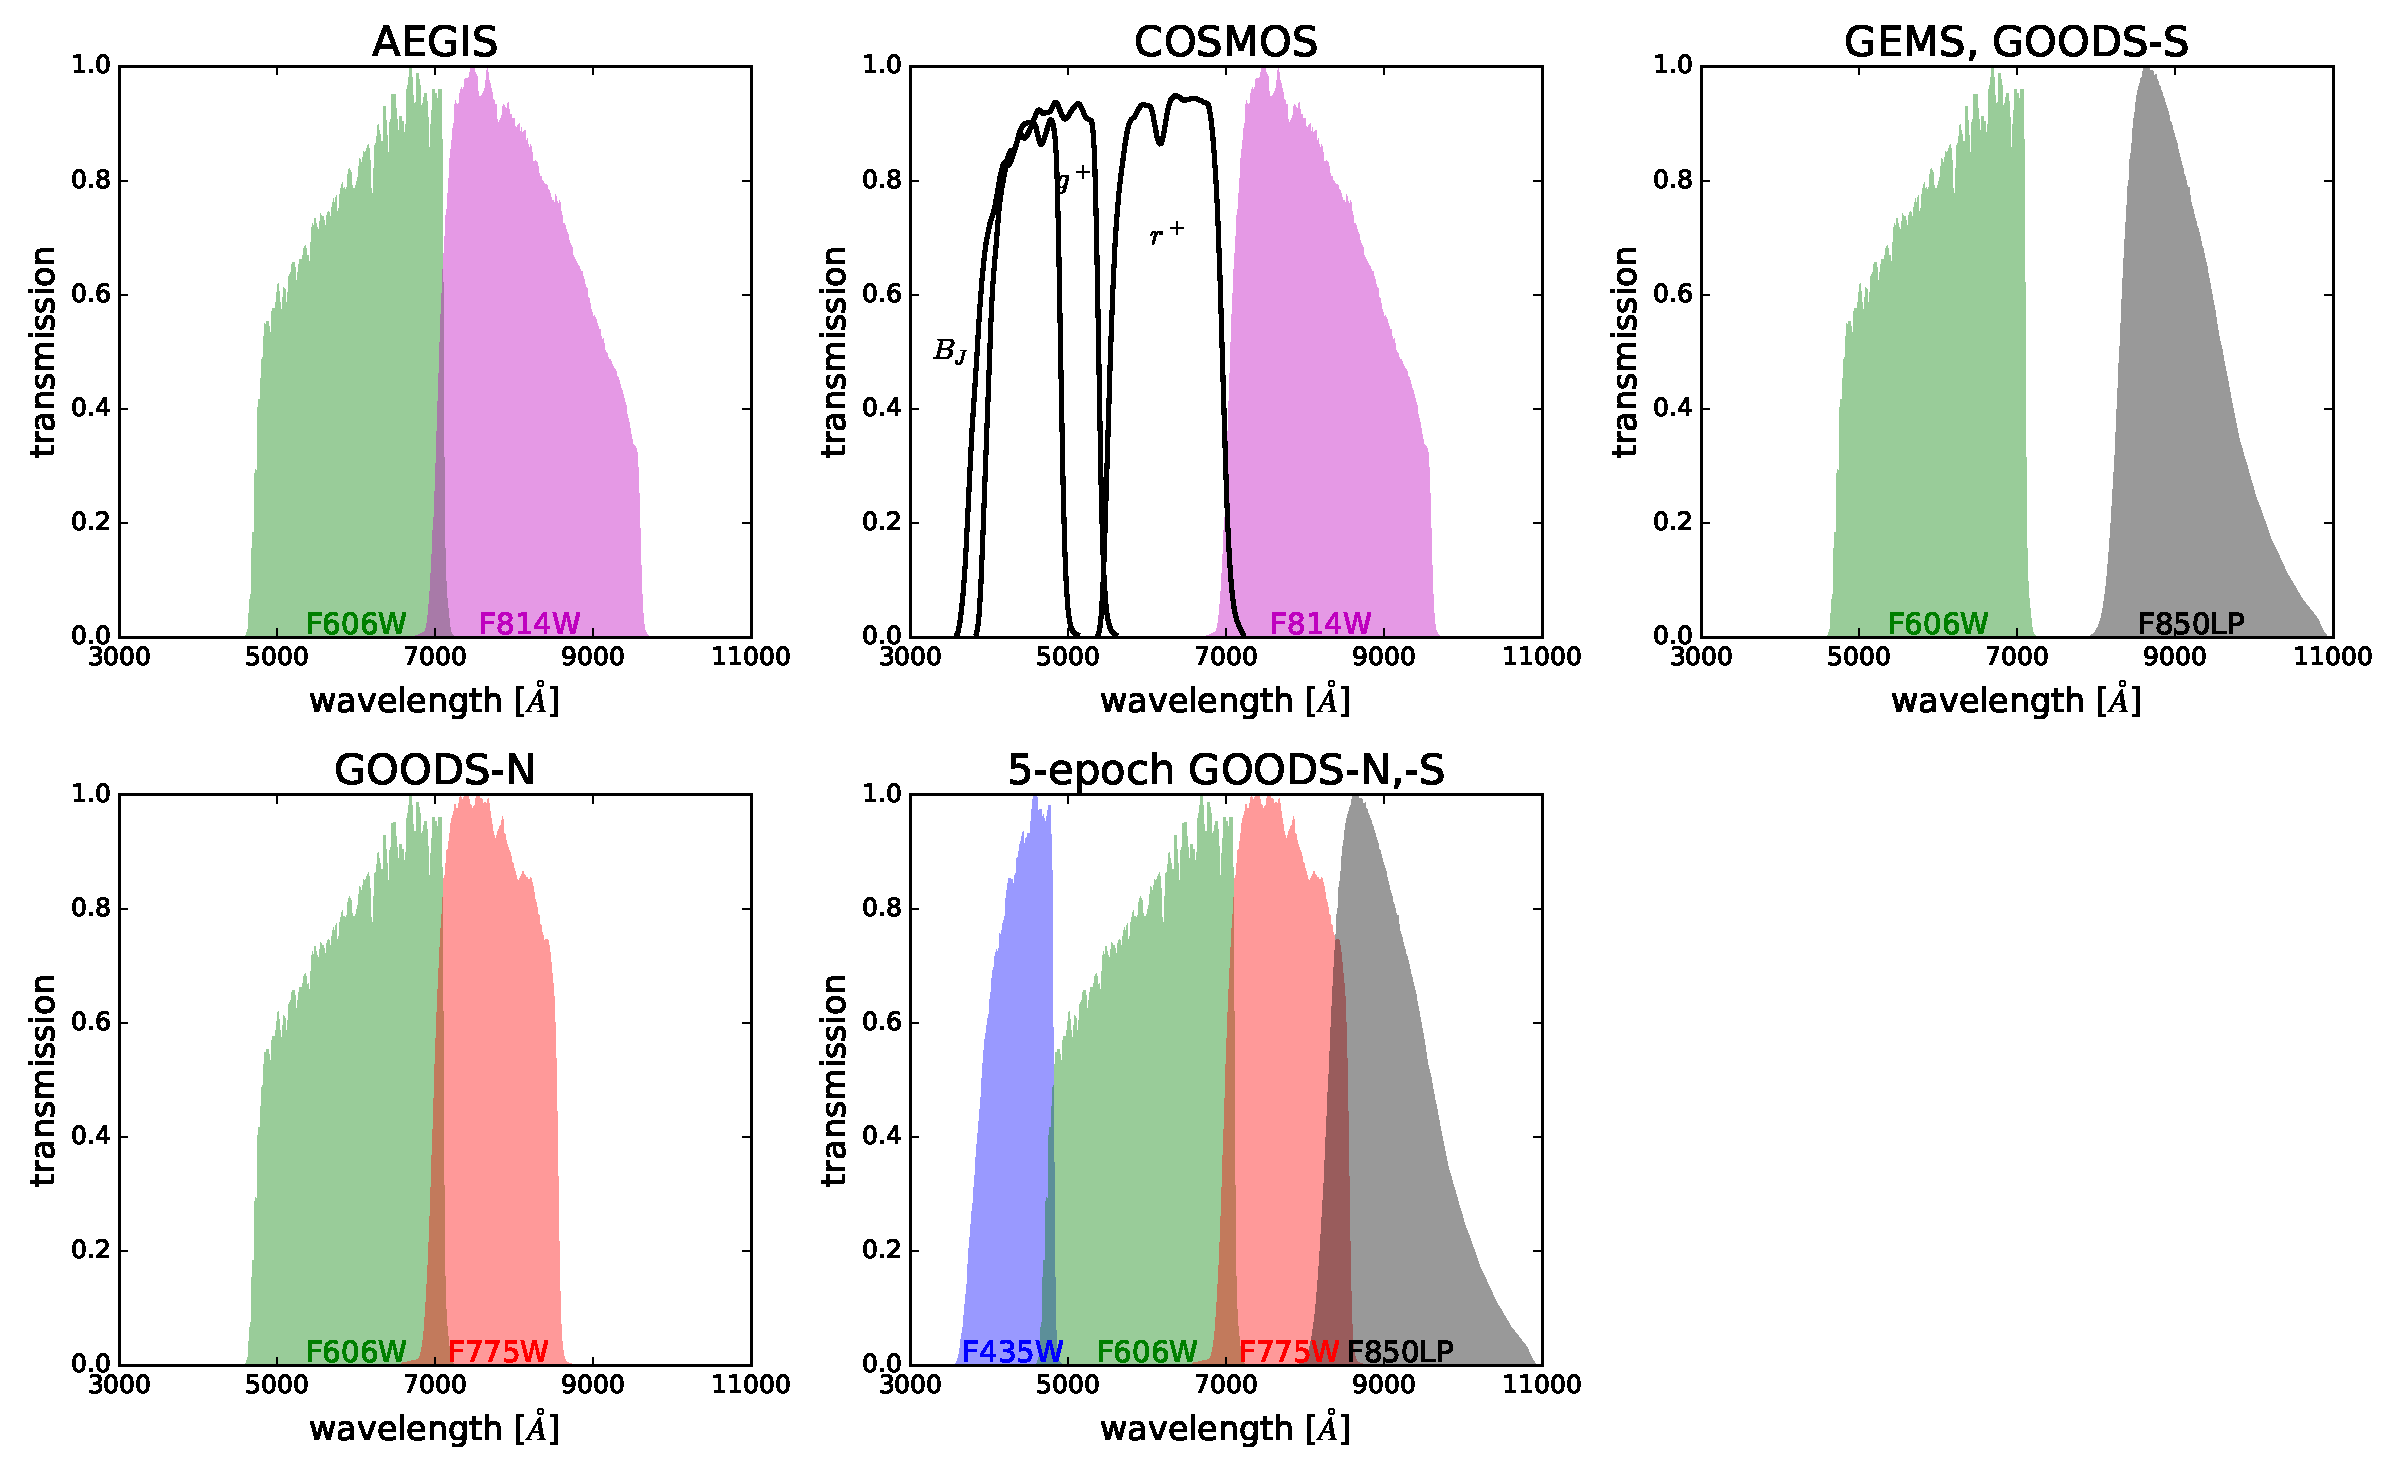
\includegraphics[width=160mm]{figures/filter_curves.pdf}
\caption{Transmission curves of the filters used by \hst{} Advanced Camera for
Surveys (ACS) in wide-field channel mode for the various surveys in GZH. The
unfilled black curves show the filters for the Suprime Camera on the
\textit{Subaru} telescope, which was used to create color gradients in the GZH
images for COSMOS.\label{fig:filtercurves}}
\end{figure*}

The properties of the individual surveys are as follows:

\begin{itemize}

\item The All-Wavelength Extended Groth Strip International Survey
    \citep[AEGIS;][]{dav07} covers a strip centered at
    $\alpha=14^\textrm{h}17^\textrm{m}, \delta=+52^\circ30^\prime$. This area
    of the sky was selected for a deep survey due to a combination of low
    extinction and low Galactic/zodiacal emission. The ACS images covered 63
    separate tiles over a total area of $\sim710$~arcmin$^2$. The two ACS bands
    for AEGIS had exposure times of 2300~seconds in F606W (\Vband) and
    2100~seconds in F814W (\Iband). The final mosaic images were dithered
    to a resolution of 0.03~\arcsec/pixel. For extended objects, the
    limiting magnitude of sources was 26.23~(AB) in \Vband{} and 25.61 (AB) in
    \Iband. 

\item The Great Observatories Origins Deep Survey \citep[GOODS;][]{gia04}
    covered two separate fields in the northern and southern hemispheres: the Hubble
    Deep Field-North ($\alpha=12^\textrm{h}36^\textrm{m},
    \delta=+62^\circ14^\prime$) and the Chandra Deep Field-South
    ($\alpha=03^\textrm{h}32^\textrm{m}, \delta=-27^\circ48^\prime$). The \hst{}
    ACS imaging data from the two fields are referred to as GOODS-N and GOODS-S,
    respectively. ACS imaging in GOODS fields used 4 filters -- F435W (\Bband),
    \Vband, F775W (\iband), and F850LP (\zband). The mean exposure times for each
    epoch varied by band, from 1050--2100~seconds. The \Bband{} images were completed
    in a single epoch at the beginning of the survey, but the \Vband, \iband, and
    \zband{} images were taken in five separate epochs separated by 40--50~days
    each. Images were dithered to a pixel scale of 0.03~\arcsec/pixel and covered a
    total area of $\sim320$~arcmin$^2$ (160~arcmin$^2$ per north/south field). The
    $5\sigma$ limiting magnitude for extended sources was 25.7 for \Vband{} and
    25.0 for \iband. 

\item The Cosmic Evolution Survey \citep[COSMOS;][]{sco07} covered an area of
    $\sim1.8$~deg$^2$ centered at $\alpha=10^\textrm{h}00^\textrm{m},
    \delta=+02^\circ12^\prime$. Its location near the celestial equator was
    designed to enable coverage by ground-based telescopes in both the Northern and
    Southern Hemispheres, in addition to space-based observatories. The ACS data
    for COSMOS consisted of 1~orbit per pointing with an exposure time of
    2028~seconds in \Iband; 590 total pointings were used to cover the entire
    field. The image resolution was dithered to 0.05~\arcsec/pixel. The 50\%
    completeness magnitude for a galaxy with a half-light radius of
    $0.50^{\prime\prime}$ in \Iband{} was 24.7 mag. 

\item The Galaxy Evolution from Morphologies and SEDs
    \citep[GEMS;][]{rix04,cal08} survey was also centered on the Chandra Deep
    Field-South. The GEMS data covered $\sim800$~arcmin$^2$, completely surrounding
    the area covered by GOODS-S. Images from ACS in GEMS had 1 orbit per pointing
    for a total of 63~pointings. The exposure times were 2160 and 2286~seconds in
    \Vband{} and \zband{}, respectively. The image resolution had a pixel scale
    of 0.03~\arcsec/pixel. The $5\sigma$ limiting magnitude for source
    detection was 25.7 AB in \Vband{} and 24.2~AB in \zband. 

\end{itemize}

% Note: galaxy counts remove the duplicate observations from gz_hst_table

\begin{table*}
\center
\caption{Summary of GZH imaging \label{tbl:gzh_numbers}}
\begin{tabular}{lllcrr}
\hline\hline
Survey &  Total $t_{\rm exp}$ & Filters & Resolution & Area & $N_{\rm galaxies}$ \\
 & [sec] & & [\arcsec/pix] & [arcmin$^2$] & \\
\hline
AEGIS                                   & 2100$-$2300  & \Vband, \Iband{}                 & 0.03 & 710                & 8157    \\
COSMOS                                  & 2028         & \Iband{}                         & 0.05 & 6480               & 88530   \\
GEMS                                    & 2160$-$2286  & \Vband, \zband{}                 & 0.03 & 800                & 9143    \\
GOODS                                   & $-$          & $-$                              & $-$  & $-$                & $-$     \\
\hspace{10pt} \emph{GOODS-N~2~epoch}    & 2100$-$4200  & \Vband, \iband                   & 0.03 & 320                & 2551    \\
\hspace{10pt} \emph{GOODS-S~2~epoch}    & 2100$-$4200  & \Vband, \zband                   & 0.03 & 320                & 3593    \\
\hspace{10pt} \emph{GOODS-N~5~epoch}    & 5100$-$10500 & \Bband, \Vband, \iband, \zband{} & 0.03 & $^{\prime\prime}$  & 6015    \\
\hspace{10pt} \emph{GOODS-S~5~epoch}    & 5100$-$10500 & \Bband, \Vband, \iband, \zband{} & 0.03 & $^{\prime\prime}$  & 5142    \\
\hline
total                                   & $-$          & $-$                              & $-$  & 8630 & 123131  \\
\hline\hline
\end{tabular}
\end{table*}

\subsection{Galaxy selection}

In the ACS-GC \citep{gri12}, individual galaxies were identified using a
combination of \sextractor{} \citep{ber96} and the galaxy-profile fitting
framework \galapagos{} \citep{bar12}. GZH included all galaxies with $m<23.5$,
where $m$ is in the \Iband, \zband, or \iband{} for the AEGIS + COSMOS, GEMS +
GOODS-S, and GOODS-N surveys, respectively. This yielded a total of
113,166~images (Table~\ref{tbl:gzh_numbers}).

Single-epoch images from SDSS Stripe~82 were selected using the same criteria
from \citet{wil13}, which required limits of \texttt{petroR90\_r}$ >
3$\arcsec~(where \texttt{petroR90\_r} is the radius containing 90\% of the
$r^\prime$ Petrosian flux) and a magnitude brighter than $m_r < 17.77$. The
images used were three-color composites using the $g^\prime$, $r^\prime$, and
$i^\prime$ filters \citep{nie04}. 21,522 galaxies in SDSS met these criteria.
Co-added images from Stripe~82 were selected from the union of galaxies with
co-added magnitudes brighter than $17.77$~mag, and the galaxies detected in the
single-depth images and matched to a co-add source. This resulted in a total
set of 30,339 images. Of the images in the co-added sample, 5144 (17~percent)
were dimmer than the initial magnitude cut of 17.77. 

\subsection{Image creation}

The images used for classification in GZH were color-composite JPGs made from
multi-band data. The exact process for creating the images depended on the bands
and resolutions in the surveys. 

For galaxies in the ACS-GC, color composites were made using a fixed pixel
intensity scaling with weights of
$[2.4\times10^{-4},3\times10^{-4},3\times10^{-4}]$ in the red, green, and blue
channels respectively. A nonlinear mapping was applied to each pixel to
emphasize the contrast in faint features \citep{lup04}, taking the form of:

\begin{equation}
I_\mathrm{channel,new} = I_\mathrm{channel,old} \times \frac{\arcsinh(b\times r)}{(b\times r)}
\label{eqn:nonlinear}
\end{equation}

\noindent GZH images from \citet{gri12} used a value of $b=3$. 

The majority of the data in Legacy surveys described in
Section~\ref{ssec:legacy_surveys} had images in only one or two filters
available when the GZH project was first launched, making standard 3-channel
RGB images in the same method used for the SDSS images in the original Galaxy
Zoo impossible. For surveys with images in two bands (AEGIS, GEMS, and the
two-epoch GOODS-N and GOODS-S), the lower-wavelength band was mapped to the
blue channel, the higher-wavelength band to the red channel, and the green
channel created by taking the geometric mean of the two. Bands used in each of
the surveys are listed in Table~\ref{tbl:gzh_numbers}. The 2-epoch GOODS-N and
GOODS-S images used different filters --- this was a deliberate choice made so
that the GEMS images could be directly compared with the overlapping coverage
of GOODS-S (Figure~\ref{fig:filtercurves}). 

By the time that the 5-epoch sets of GOODS data were put into GZH (in March
2015), coverage in four separate \hst{} bands were publicly available. The
deeper GOODS images were created using the arithmetic mean of \Bband{} and
\Vband{} in the blue channel, \Iband{} in the red channel, and \zband{} in the
green channel. These images also had their speckled noise pixels decolorized. 

The COSMOS images only had the \Iband{} imaging available at the time of
classification in GZH. For these galaxies, GZH used ``pseudocolor'' images
created by using the ACS \Iband{} data as an illumination map and ground-based
imaging from the \subaru{} telescope in $B_J$, $r^+$, and $i^+$ filters to
provide the color gradients \citep[see][for further details]{gri12}. This
resulted in images with the angular resolution of \hst{}
($\sim0.05$~\arcsec/pixel) for the overall intensity, but color gradients at
ground-based resolution, with seeing between 0.95\arcsec{} and 1.05\arcsec{}
\citep{tan07}.

Stripe~82 single-epoch images were taken directly from the DR7 SDSS Skyserver,
which combined $g^{\prime}$, $r^{\prime}$, and $i^{\prime}$ exposures into the
RGB channels. The co-added Stripe~82 images were assembled from runs 106 and
206 in DR7 and made into color composites using the method of \citet{lup04}.

To deal with situations in which the sky noise was highly colored (which might
have been a distraction to visual classification), a soft-edged object mask was
applied to the coadded Stripe~82 and the COSMOS images. This mask preserved the
color balance for galaxies, but desaturated speckled noise against regions of
blank sky.

\subsection{Images with simulated nuclear point sources}

GZH also included a set of images designed to measure the effect of active
galactic nuclei (AGN) on morphological classifications. Since galactic nuclei
can have bright, unresolved optical emission, AGN have the potential to mimic
or distort the identification of a bulge component. The presence of an AGN was
simulated by modeling the point spread function (PSF) of the telescope and then
inserting a bright source near the center of a real galaxy. For each image, the
simulated AGN was assigned one of three colors -- either blue, red, or flat
(white) as seen in the color images -- and a range of brightnesses such that
$L_\mathrm{ratio} \equiv L_\mathrm{galaxy}/L_\mathrm{AGN}$ is in
$(0.2,1.0,2.0,5.0,10.0,50.0)$. Combining these parameters generated 15~images
with different simulated AGN for each host. 

Two sets of simulated AGN were generated in GZH. The first set (version~1) was
assembled from 95~galaxies from GOODS-S imaging and empirical PSFs made by combining stars in the GOODS fields using the PSF creation tools in \texttt{daophot}. 
The second set (version~2) was assembled from 96~galaxies in GOODS-S; this
version used simulated PSFs from \texttt{TinyTim} \citep{kri93}, drizzled using the same procedures as those used in reduction of the GOODS-S images \citep{koe02,koe03,gia04}. The use of these 2 versions facilitates comparisons between these different PSF creation methods, which are widely used in AGN host galaxy morphology studies \citep[e.g.,][]{san04,sim08,pie10a,simm11}. 
% okay so I'm a cheeky self-citing biyotch
Each PSF creation method has advantages and disadvantages: the empirical PSFs better represent the nuances of the PSF in the specific data being used and look more realistic at lower luminosities, but the extended features of the noiseless \texttt{TinyTim} PSFs are visually more realistic at higher luminosities.

Images with simulated AGN were classified in the main interface in an identical
manner and evenly distributed with unaltered images of the galaxies.
Classifiers were not explicitly told that the images had been altered during classification, as the
goal was to measure the effect on normal classifications in as unbiased a
manner as possible. Following classification, a classifier could view a page with additional details about each galaxy they had classified; where applicable these pages contained further information regarding image modifications.

\subsection{Galaxy metadata}

Photometric data for the bulk of the GZH sample were largely drawn from the
tables in \citet{gri12}. This included photometric parameters such as
the fluxes, magnitudes, radii, ellipticities, position angles, and positions
drawn from both \sextractor{} and \galfit. \galfit{} also provided the
parametric \sersic{} index and effective half-light radius for the best-fit
model. All parameters were measured in both bands of the ACS imaging, with the
exception of the single-band COSMOS images.

Redshifts for the GZH catalog were compiled from a variety of sources. For each
galaxy, the primary redshift used for debiasing calculations
(Section~\ref{sec:debiasing}) is in the $\tt Z\_BEST$ column of
Table~\ref{tbl:catalog_hst}. The redshift type (spectroscopic: $\tt SPEC\_Z$,
photometric: $\tt PHOTO\_Z$, or grism: $ \tt GRISM\_Z$) is listed in the column
$\tt Z\_BEST\_TYPE$, and the source catalog of the redshift is included as $\tt
Z\_BEST\_SOURCE$. 

For galaxies which have published redshifts from multiple sources, the
following algorithm was used to select the $\tt Z\_BEST$ quantity. The first
priority is spectroscopic redshifts; these were taken from the ACS-GC
\citep{gri12}, 3DHST \citep{mom15}, and MUSYC \citep{car10} catalogs. A
high-quality spectroscopic redshift in the ACS-GC is the primary option; if
none is available, then $\tt Z\_BEST$ uses the spectroscopic redshifts in
3DHST, and then MUSYC. For galaxies with multiple spectroscopic redshifts, more
than 98\% are consistent at $\Delta z<0.001$, and so the order of selection
made no practical difference. Those which are inconsistent ($\Delta z>0.001$) between any of the three catalogs are marked with a Boolean flag in the column $\tt z\_spec\_conflict\_flag$ in Table~\ref{tbl:catalog_hst}. If no spectroscopic redshifts were available,
the 1-$\sigma$ errors of the photometric \citep[ACS-GC, 3DHST, MUSYC,
UltraVISTA;][]{ilb13} and UltraVISTA grism data were used to select the
redshift with the smallest error. 
%Table~\ref{tbl:redshifts} shows the results of this selection. 
 
%\begin{figure*}
%\center
%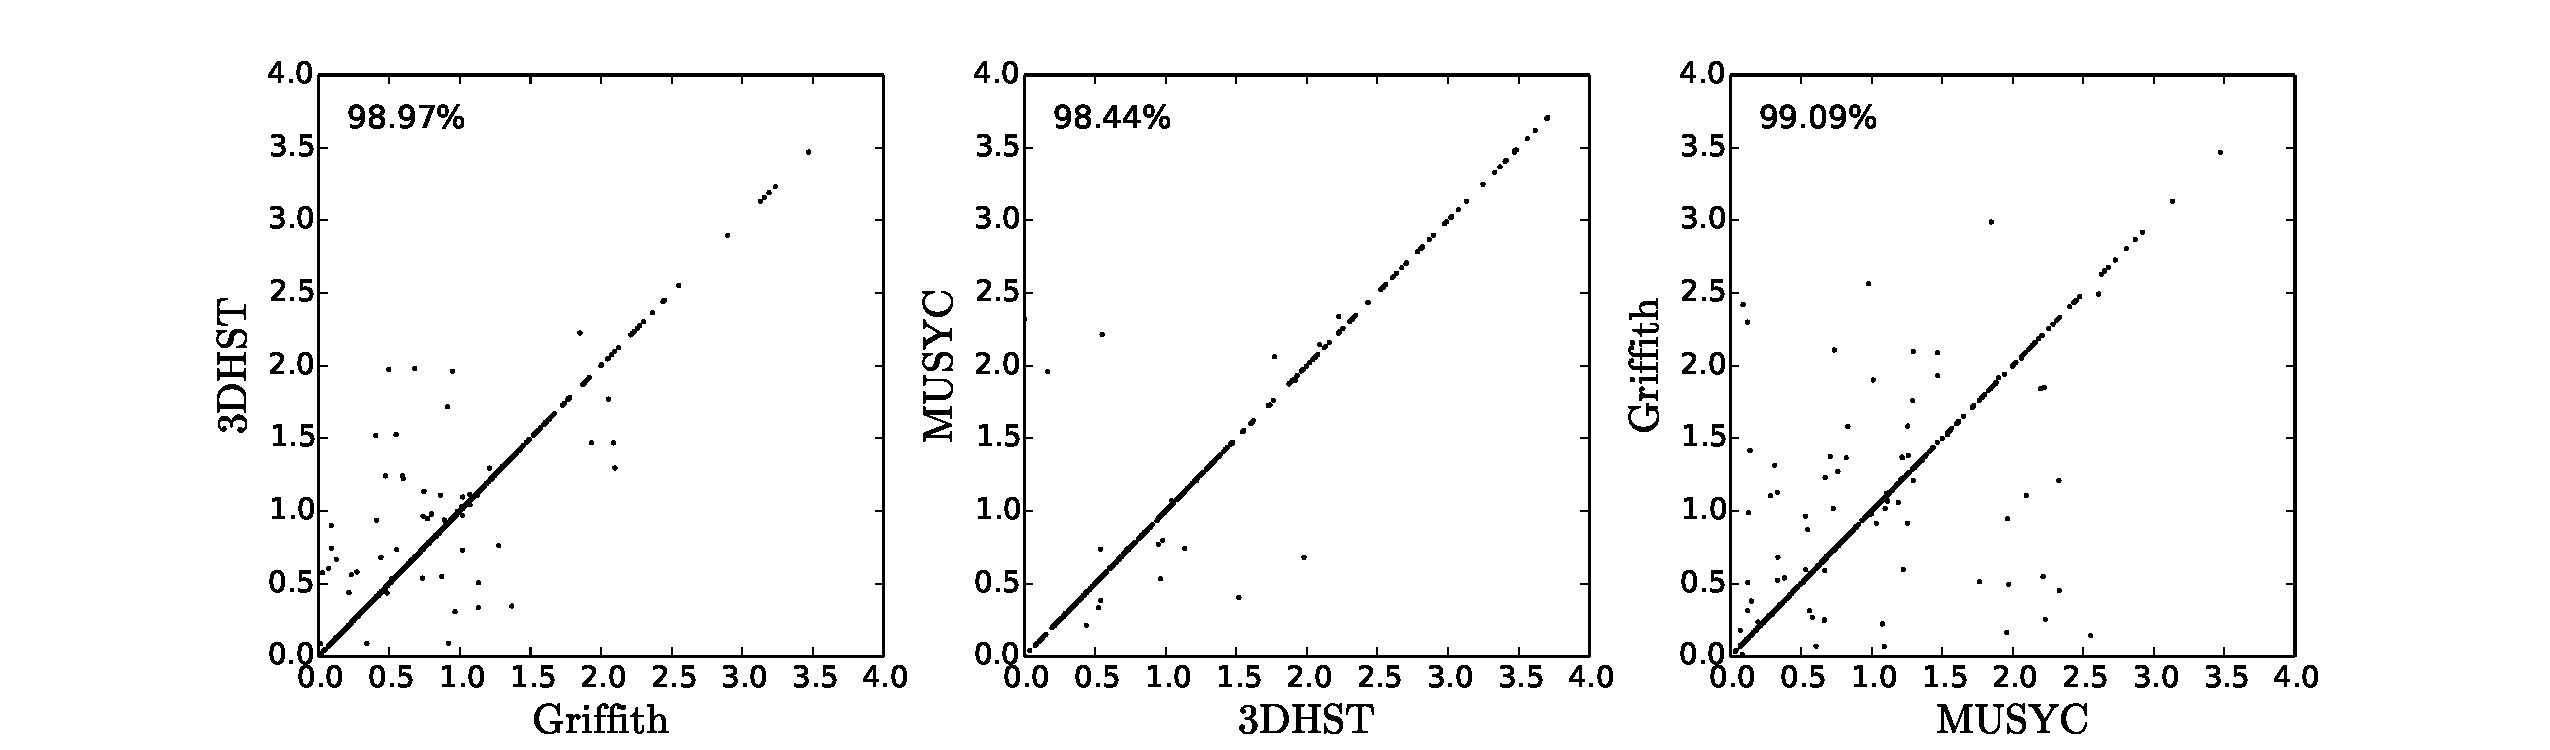
\includegraphics[width=160mm]{figures/specz_comparison.pdf}
%\caption{Spectroscopic redshifts from the ACS-GC, 3DHST, and MUSYC catalogs.
%The number in the upper left of each plot is the percentage of redshifts which
%agree within $\Delta z < 0.05$ between the two catalogs being compared in each
%panel. Within this range there is over 98\% agreement in redshifts between all
%three catalogs.}
%\label{fig:speczs}
%\end{figure*}


%\tabletypesize{\scriptsize}
%\begin{deluxetable*}{l|rr|rrr|rr|r|rr}
%\tablecolumns{12}
%\tablewidth{0pc}
%\tablecaption{GZH redshifts by survey\label{tbl:redshifts}} 
%\tabletypesize{\scriptsize}
%\tablehead{
% &   
%\multicolumn{2}{c}{\underline{ACS-GC}} &
%\multicolumn{3}{c}{\underline{3DHST}} &
%\multicolumn{2}{c}{\underline{MUSYC}} &
%\multicolumn{1}{c}{\underline{UltraVISTA}}&
%\multicolumn{2}{c}{\underline{Total}} 
%\\
%\colhead{Survey} & 
%\colhead{spec-z} & 
%\colhead{photo-z} & 
%\colhead{spec-z} & 
%\colhead{grism-z} & 
%\colhead{photo-z} & 
%\colhead{spec-z} & 
%\colhead{photo-z} & 
%\colhead{photo-z} & 
%\colhead{with redshift} &
%\colhead{in survey}
%}
%\small
%\startdata
%%Survey     Gs        Gp    3ds    3dg     3dp       Ms      Mp       UVp       total
%AEGIS    & 3,656  & 2,941  & 12  &  515  &  249    & 0     & 0     &  0      & 7,373   & 8,507   \\
%COSMOS   & 7,201  & 77,435 & 35  &  358  &  26     & 0     & 0     &  2,665  & 85,020  & 92,808  \\
%GEMS     & 387    & 628    & 6   &  99   &  40     & 279   & 7,304 & 0       & 8,743   & 9,304   \\
%GOODS-N  & 1,947  & 37     & 418 & 1,545 &  1,381  & 0     & 0     & 0       & 5,328   & 12,030  \\
%GOODS-S  & 1,080  & 4      & 327 & 1,348 &  281    & 816   & 1,184 & 0       & 5,040   & 10,284  \\
%SDSS     & 0      & 0      & 0   &  0    &  0      & 0     & 0     & 0       & 37,545  & 51,861  \\
%\hline
%Total    & 14,271 & 81,045 & 798 & 3,865 & 1,977   & 1,095 & 8,488 & 2,665   & 114,204 & 184,794 \\
%\enddata
%\end{deluxetable*}

Photometric and spectroscopic data for the SDSS Stripe~82 galaxies were taken
from the CasJobs DR7 tables. This included $ugriz$ Petrosian magnitudes and
fluxes, as well as the relative de~Vaucouleurs and exponential fits from the
model magnitudes. All redshifts used for SDSS galaxies were spectroscopic.
82.6\% of galaxies in the single-depth images and 65.1\% of galaxies in the
co-add images had a measured DR7 spectroscopic redshift. 

\section{GZH interface and classifications}\label{sec:interface}

\subsection{Classifier weighting}\label{ssec:weighting}

The votes of individual classifiers in GZH were combined to make a vote
fraction for each response ($f_{response}$) to a question in the classification
tree. Votes were weighted in a method similar that in previous versions of
Galaxy~Zoo \citep{lan08,wil13}, such that classifiers who frequently disagreed
with others ended up having very low weights. The weighting $(w)$ was 1 for the
top 95\% of classifiers, as ranked by consistency. For the bottom 5\% of
classifiers, $w$ was designed to drop smoothly and was effectively zero for the
bottom 1\%.  Since this only affected a tiny percentage of the classifiers (and
an even smaller percentage of the classifications) the overall effect on the
GZH dataset was minimal. The method was effective, however, at filtering out
contributions from random or deliberately malicious classifiers.

Classifications were aggregated and weighted only if the classifier was logged
into GZH under their username (which was encouraged, but not required for
participation). Classifications by participants who were not logged in were marked as
``Anonymous''; no weighting was applied, but the data were otherwise treated
identically in the data processing. 

\subsection{Interface and decision tree}\label{ssec:interface}

\begin{figure*}
\center
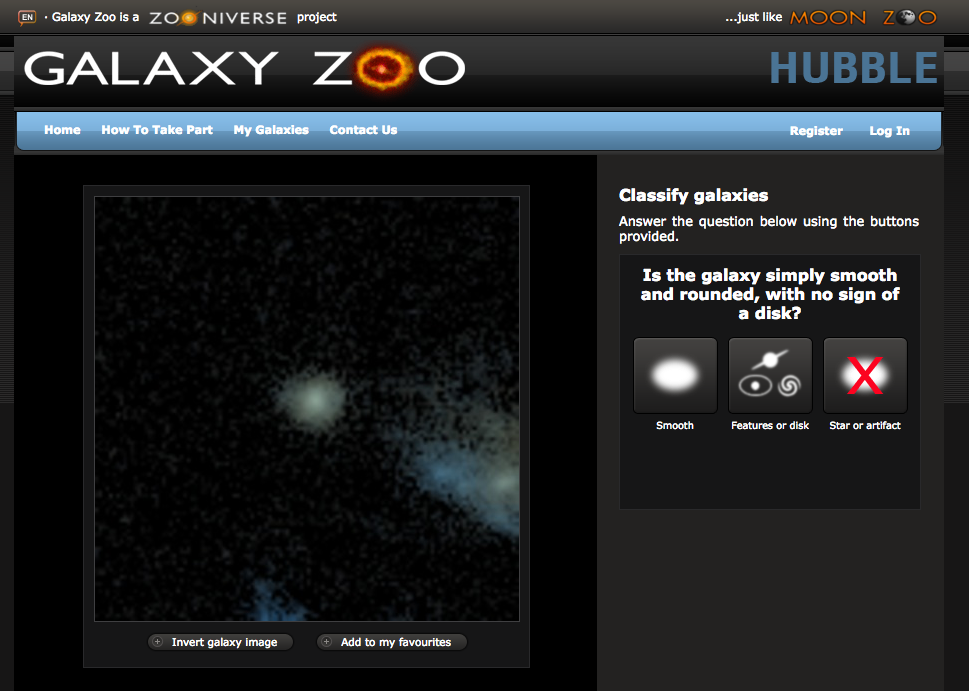
\includegraphics[width=160mm]{figures/gzh_interface.png}
\caption{Screenshot of the GZH interface (\url{http:/zoo3.galaxyzoo.org}) at
the beginning of a classification, with the classifier ready to select an answer for
the first question in the decision tree.\label{fig:interface}}
\end{figure*}

Classifications for GZH were made using a web-based interface
(Figure~\ref{fig:interface}), similar in design to Galaxy~Zoo and Galaxy~Zoo~2.
The front-end runs on a Ruby~on~Rails framework with classifications stored in
a MySQL backend. Classifiers were shown a randomly-selected color composite image from
the GZH sample; the default showed the image with a black sky background,
although they had the option to invert the color palette if desired. The
questions and responses for morphology appeared on the right side of the image as
a panel, including both text and icons. There was no tutorial required for
participation, although classifiers could access an extensive ``Help'' section
containing example images and descriptive text for all the morphological
labels. 

\begin{figure*}
\center
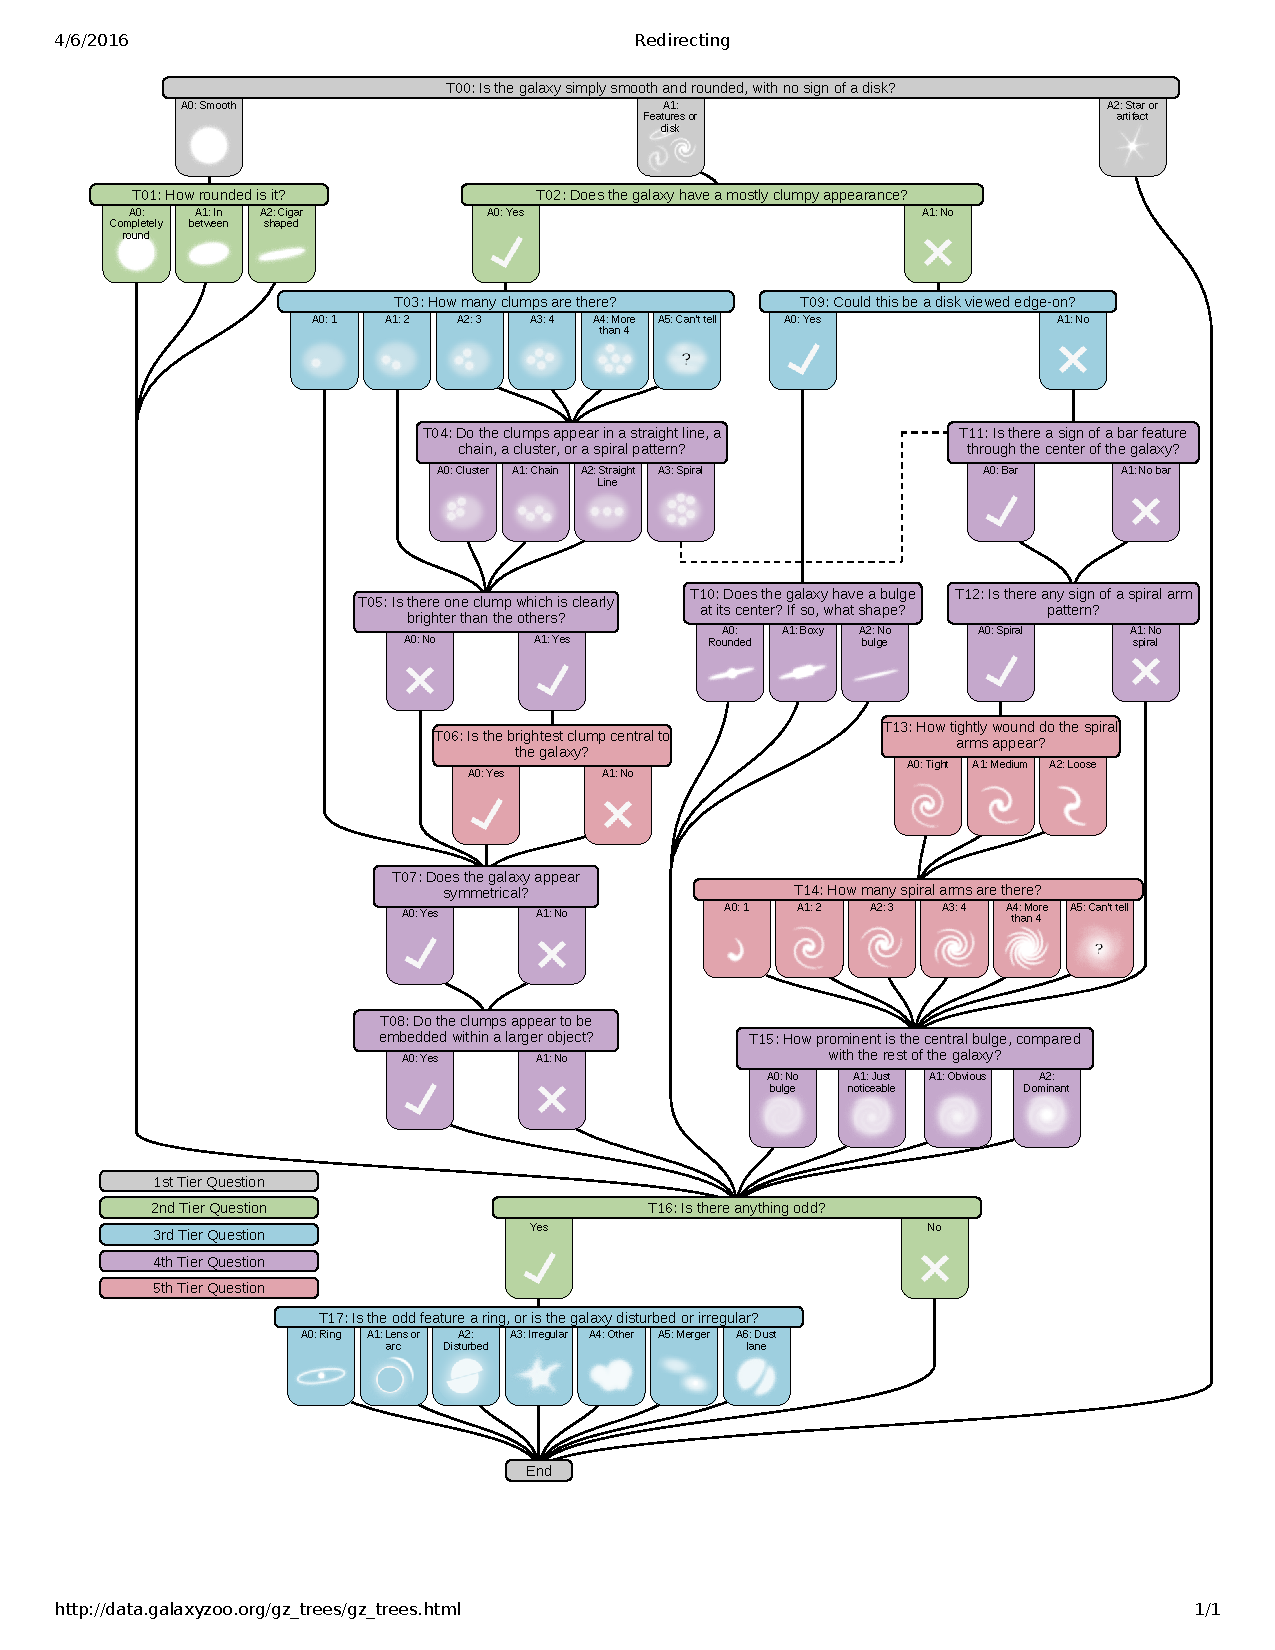
\includegraphics[width=\textwidth]{figures/gzh_decision_tree.pdf}
\caption{Flowchart of the questions presented to GZH classifiers, labeled with
the corresponding Task numbers. Tasks in the decision tree are color-coded by
tier level: Gray-colored Tasks are 1$^\mathrm{st}$-tier questions which are
asked in every classification. Tasks colored green, blue, purple, and pink
(respectively) are one, two, three, or four steps below branching points in the
decision tree.}
\label{fig:decisiontree}
\end{figure*}

The procedure for classifying an image in GZH followed a hierarchical decision
tree (Figure~\ref{fig:decisiontree}). Every classification began with the step of
identifying whether the object at the center of the image was a smooth galaxy,
a galaxy with a disk or other features, or a star/artifact. Subsequent
questions in the tree depended on the previous answer(s) given by the classifier; the
decision tree was designed so that every question relevant to
the morphology in the process of being identified was answered. Questions that were not
answered were implicitly assumed to be absent in the image --- for example, if
the classifier identified a galaxy as being smooth, they were not asked to count the
number of spiral arms. For every task, the classifier chose a single answer before
continuing to the next question; they also had the option to restart any
classification in-progress. 

The GZH decision tree had four broad sets of morphologies. The first option
designated stars or image artifacts (the result of either bad data or incorrect
classification by the ACS pipeline as a galaxy); in this case, the
classification process ended and no further questions were asked. The second
set were smooth galaxies, intended to select ellipticals/early-types;
classifiers also measured the relative axial ratio (roundness) for these
galaxies. The third set was for disk/late-type galaxies, which measured the
features necessary to place a galaxy on the standard Hubble tuning fork (bars,
spiral arm, strength of the central bulge). The final set, which was new in
this phase of Galaxy~Zoo and designed for high-redshift targets, identified
objects dominated by clumpy morphologies. Further annotations for clumpy
galaxies included assessing the number, arrangement, relative brightness, and
location of the clumps within the galaxy. Finally, every classification of a
galaxy gave the option of identifying ``odd'' features within the image; these
labels were for relatively rare $(\lesssim1\%)$ phenomena, including dust
lanes, gravitational lenses, and mergers. 

The number of independent classifications per subject collected by GZH was on
average higher than GZ1 or GZ2, due to both the increased complexity of the
decision tree and the relative difficulty of classifying images of small and
distant galaxies. Images from the main AEGIS, GEMS, and GOODS data sets had a
median of 122~independent classifications per image. The remainder of the
images either had a later activation date (COSMOS, simulated AGN) or a lower
retirement limit (the low-redshift SDSS Stripe~82 galaxies). Images from these
samples had a median of 46--48~classifications per image
(Figure~\ref{fig:classification_hist}).

\begin{figure}
\center
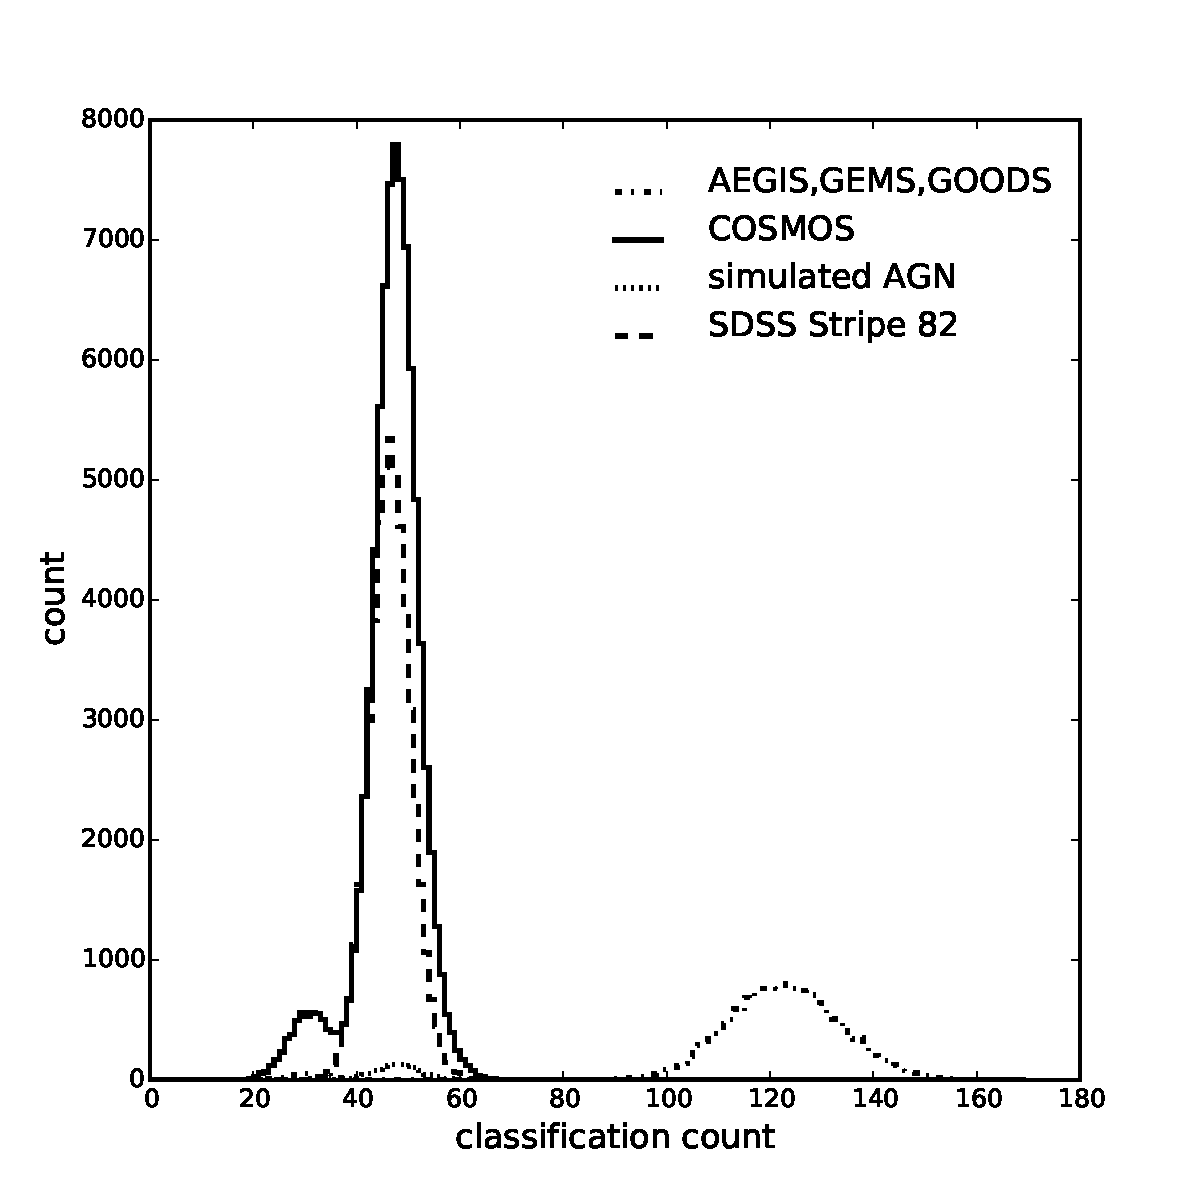
\includegraphics[width=0.5\textwidth]{figures/classification_hist.pdf}
\caption{Distribution of the total number of classifications per image for GZH,
split by survey.}
\label{fig:classification_hist}
\end{figure}

The GZH project was launched on 23~Apr~2010 with the inclusion of the AEGIS,
GEMS, GOODS 2-epoch, and SDSS Stripe~82 images. Images from COSMOS and the
simulated AGN were activated in Dec 2010, as well as a small sample of
AEGIS/GEMS/GOODS images mistakenly excluded from the original sample based on
an overly restrictive cut on blended and/or saturated objects. The main GZH
site collected data until its replacement, the fourth phase of
Galaxy~Zoo\footnote{\url{http://zoo4.galaxyzoo.org}} (including data from both
the \hst{} CANDELS survey and SDSS DR8) began on 10~Sep~2012. Classifications
for the GOODS 5-epoch images were separately obtained from Mar-Jun 2015 on
the fourth version of the Galaxy~Zoo site. The GZH project had a total of
10,349,357~classifications from 93,898 registered participants. 
% Sum is the total of the GZH SQL table plus the GOODS full-depth imaging in GZ4.

\section{Correcting for redshift-dependent classification bias}\label{sec:debiasing}

The previous versions of Galaxy Zoo morphology classifications
\citep{lin08,wil13} were based on observations of galaxies in the Sloan Digital
Sky Survey (SDSS) which have a median redshift of $z<0.2$. In these cases, it
was assumed that there was no cosmological evolution of the morphologies of
galaxies and therefore any observed changes in the distribution of galaxies
with different consensus morphologies was due to the effects of redshift on the
image quality (\ie, the reduction in physical resolution, surface brightness
dimming, etc). For both previous releases of GZ morphologies, a correction for
redshift-dependent bias was applied based on matching the classification
fractions at the highest redshifts with those at the lowest redshift.
\citet{bam09} and \citet{wil13} provide complete descriptions of the process
for GZ1 and GZ2, respectively.

In the GZH samples, the redshift range is large enough that cosmological
evolution of the types and morphologies of galaxies is expected for galaxies in
the sample. As a result, the previous methods of correcting for redshift
dependent bias do not work. In addition, the effects of band shifting will
change the images even more across these redshift ranges. 
%Figure~\ref{fig:exampleFERENGI} illustrates some of the possible effects of
%losing features in spiral galaxies at high redshift. 

In order to test and correct for the effects of redshift, GZH includes a set of
calibration images. These images consist of the same galaxy as it would appear
over a variety of redshifts. The input images are from the SDSS
\citep{yor00,str02} and are processed using the \ferengi{} code \citep{bar08a}
to match the observational properties of the \hst{} surveys out to $z=1$. These
images were classified in the GZH interface using the same classification
scheme as the original \hst{} images.
 
\subsection{Generating images of artificially-redshifted galaxies}

The GZH classifications include 288 unique galaxies originally generated from
SDSS imaging and processed with the \ferengi{} code. The selection spanned a
variety of galaxy morphologies (as selected by GZ2 classifications) and
$r^\prime$-band surface brightnesses, and also spanned the redshift range of
SDSS targets (in $N_z = 4$ bins) in order to be optimized for different target
minimum redshifts in \hst{} imaging. 

%The selection criteria for the different morphological categories is summarized in Table \ref{tbl:morphologies}. 
The surface brightness selection ($N_\mu = 3$) for the \ferengi{} galaxies was
(1) low: $\mu > 21.5$~\magarc;  (2) mid: $20.5 < \mu < 21.5$~\magarc; and (3)
high: $\mu < 20.5$~\magarc. For each of the four ``target redshifts''
($z_\mathrm{sim} = 0.3, 0.5, 0.8$ and $1.0$), the images were redshifted in
$\Delta z = 0.1$ bins up to $z_\mathrm{sim}=1.0$. 
 
%\begin{table*}
%\center
%\caption{Summary of morphological categories selected for \ferengi{} sample.\label{tbl:morphologies}}
%\begin{tabular}{lllc}
%\hline\hline
%Morphology          & Label &  Selection                                                                                            & $N_{\rm objects}$ \\
%                    &       &                                                                                                       & [$N_z \times N_\mu$] \\
%\hline
%Features            & Yes       & $f_{\rm features} > 0.8$, $f_{\rm odd} < 0.1$                                                         & 12 \\ 
%                    & Int.      & $0.3 < f_{\rm smooth} < 0.6$, $f_{\rm odd} < 0.1$                                                     & 12 \\ 
%                    & No        & $f_{\rm smooth} > 0.8$, $f_{\rm odd} < 0.1$                                                           & 12 \\ 
%Merger              & No        & $f_{\rm features} > 0.8$, $f_{\rm odd < 0.1}$, $f_{\rm merger} < 0.1$                                 & 12 \\
%                    & Int.      & $f_{\rm odd} > 0.5$, $0.1< f_{\rm merger} < 0.4$                                                      & 12 \\ 
%                    & Yes       & $f_{\rm odd} > 0.5$, $f_{\rm merger} > 0.4$                                                           & 12 \\
%Edge-on             & Yes       & $f_{\rm edgeon} > 0.8$, $f_{\rm features} > 0.5$                                                      & 12 \\
%                    & Int.      & $0.4 < f_{\rm edgeon} < 0.8$ , $f_{\rm features} > 0.5$                                               & 12 \\
%                    & No        & $f_{\rm edgeon} < 0.2$, $f_{\rm features} > 0.5$                                                      & 12 \\
%Bar                 & No        & $f_{\rm bar} < 0.1$, $f_{\rm features} > 0.5$, $f_{\rm edgeon} < 0.2$                                 & 24 \\
%                    & Int.      & $0.2 < f_{\rm bar} < 0.4$, $f_{\rm features} > 0.5$, $f_{\rm edgeon} < 0.2$                           & 24 \\
%                    & Yes       & $f_{\rm bar} > 0.8$, $f_{\rm features} > 0.5$, $f_{\rm edgeon} < 0.2$                                 & 24 \\
%Visible spiral      & No        & $f_{\rm spiral} < 0.2$, $f_{\rm features} > 0.5$, $f_{\rm edgeon} < 0.2$, $f_{\rm bar} < 0.1$         & 12 \\
%                    & Int.      & $0.2 < f_{\rm spiral} < 0.8$, $f_{\rm features} > 0.5$, $f_{\rm edgeon} < 0.2$, $f_{\rm bar} < 0.1$   & 12 \\
%                    & Yes       & $f_{\rm spiral} > 0.8$, $f_{\rm features} > 0.5$, $f_{\rm edgeon} < 0.2$, $f_{\rm bar} < 0.1$         & 12 \\
%Oblique bulge size  & No        & $f_{\rm nobulge>0.6}$, $f_{\rm features} > 0.5$, $f_{\rm edgeon} < 0.5$, $f_{\rm bar} < 0.2$          & 12 \\
%                    & Int.      & $f_{\rm justnoticeable}>0.6$, $f_{\rm features} > 0.5$, $f_{\rm edgeon} < 0.5$, $f_{\rm bar} < 0.2$   & 12 \\
%                    & Yes       & $f_{\rm obvious|dominant}>0.5$, $f_{\rm features} > 0.5$, $f_{\rm edgeon} < 0.5$, $f_{\rm bar} < 0.2$ & 12 \\
%Edge-on bulge shape & Round     & $f_{\rm rounded}>0.5$, $f_{\rm features} > 0.5$, $f_{\rm edgeon} > 0.5$                               & 12 \\
%                    & Boxy      & $f_{\rm boxy}>0.4$, $f_{\rm features} > 0.5$, $f_{\rm edgeon} > 0.2$                                  & 12 \\
%                    & No bulge  & $f_{\rm nobulge}>0.5$, $f_{\rm features} > 0.5$, $f_{\rm edgeon} > 0.5$                               & 12 \\
%\hline\hline
%\end{tabular}
%\end{table*}

In addition to the physical parameters of the input images, the \ferengi{}
output depends on assumptions of the global galaxy evolution model. This
evolution is a crude mechanism that mimics the brightness increase of galaxies
with increasing redshift (out to at least $z\sim1-2$). The effect on the
redshifted images is simply an empirical addition to the magnitude of a galaxy
of the form $M' = e\times z + M$, where $M'$ is the corrected magnitude, and
$e$ is the evolutionary correction in magnitudes (i.e., $e=-1$ essentially
brightens the galaxy by 1~magnitude by $z=1$). \ferengi{} was run on the images
for values of $e$ starting from $e=0$ and decreasing to $e=-3.5$ in increments
of $\Delta e = 0.5$. Figure~\ref{fig:exampleFERENGI} shows several examples
of the effects of ``losing'' spiral/disc features with increasing redshift
for two galaxies with $e=0$. 

The final number of \ferengi{} images produced for each galaxy is ultimately a
function of galaxy's redshift (since the new images cannot be resampled at
better angular resolution than the original SDSS data), as well as the number
of $e$ values selected. Table~\ref{tbl:ferengivalues} summarizes the redshifted
images produced for GZH. 

\begin{table}
\caption{Summary of \ferengi{} artificial redshifting \label{tbl:ferengivalues}}
\begin{tabular}{lccccr}
\hline\hline
$z_{\rm sim}$ & $N_{z {\rm bins}}$ & $N_{\rm evolution}$ & $e_{\rm max}$ & $N_{\rm galaxies}$ & $N_{\rm images}$\\
\hline
0.3              & 8                  & 7                   & $-3.0$        & 72             & 4032 \\
0.5              & 6                  & 4                   & $-1.5$        & 72             & 1728 \\
0.8              & 3                  & 3                   & $-1.0$        & 72             &  648 \\
1.0              & 1                  & 3                   & $-1.0$        & 72             &  216 \\
\hline\hline
\end{tabular}
\end{table}

\begin{figure*}
\center
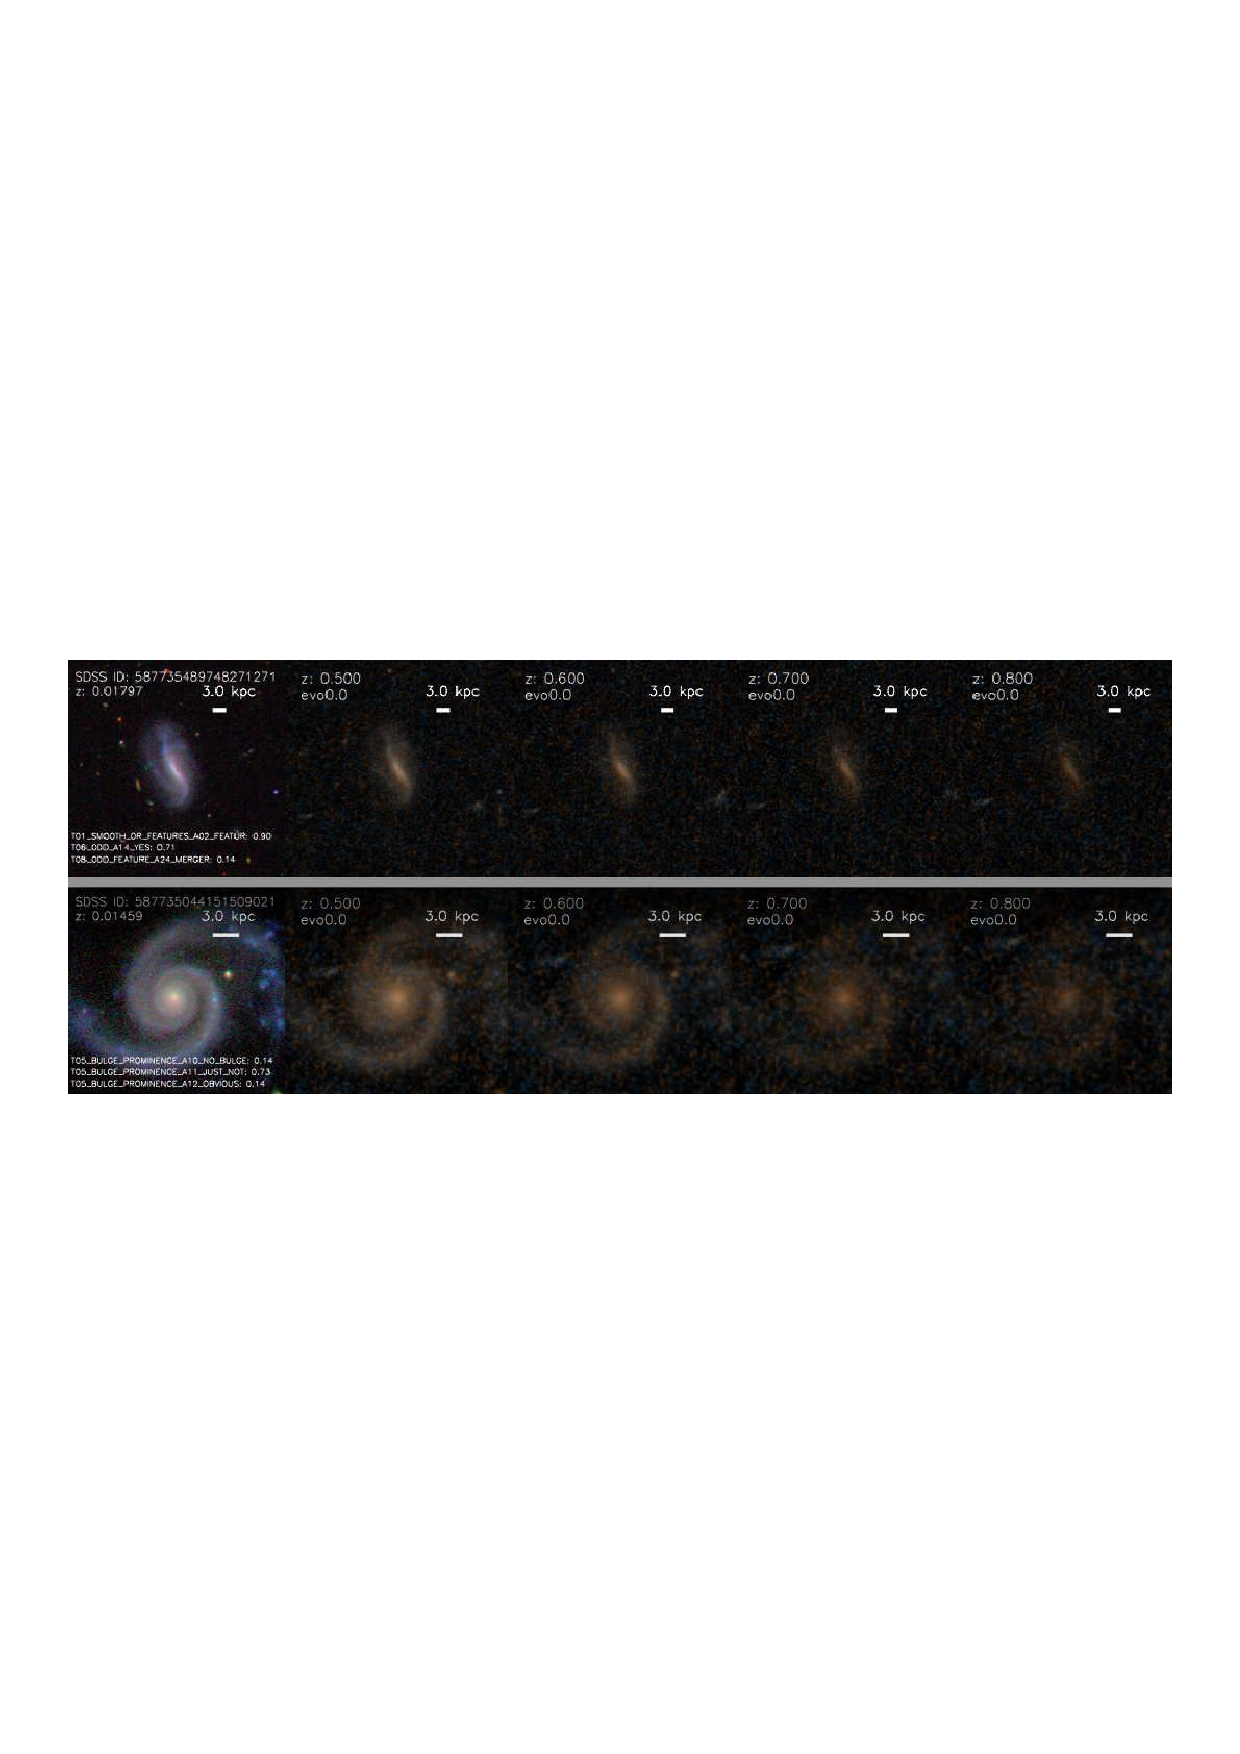
\includegraphics[width=160mm]{figures/example_ferengi.pdf}
\caption{Examples of two galaxies which have been run through the \ferengi{}
code to produce simulated \hst{} images. The measured value of \ffeatures{}
from GZH for the images in each panel are (1) Top row: \ffeatures~= (0.900,
0.625, 0.350, 0.350, 0.225) and (2) Bottom row: \ffeatures~= (1.000, 0.875,
0.875, 0.625, 0.375). \label{fig:exampleFERENGI}}
\end{figure*}

\subsection{Correcting morphologies for classification bias}\label{ssec:zeta}

The approach used in GZH for correcting the weighted classifications for redshift
bias rests on the assumption that the \emph{amount} of bias is a function of
the apparent size and brightness of the image as seen on screen. This is
controlled by two types of parameters: \textbf{intrinsic} properties of the
galaxy itself, such as its physical diameter and luminosity, and
\textbf{extrinsic} properties, such as the distance (redshift) of the galaxy
and its relative orientation. There may also be other parameters that affect
classifier accuracy, such as the proximity of close companions \citep[``distraction
bias''; see][]{joh15} or bias as a function of individual classifier ability and
skill. The combination of all such parameters forms a high-dimensional space,
and it is not clear how to separate this into individual effects. Instead, the
method used here employs only two parameters intended to capture the bulk of
the change in bias: the $r^\prime$-band surface brightness ($\mu_r$; intrinsic)
and redshift ($z$; extrinsic). 

The change in bias as a function of $\mu_r$ and \zsim{} is measured using the
\ferengi{} images over all the evolutionary correction factors. It is assumed
that the ``true'' (ie, debiased) vote fraction $f_{\mu,z}$ for a galaxy can be
expressed as:

\begin{equation}
f_{\mu,z} = \left(f_{\mu,z=0.3}\right) \times e^{{\frac{z-z_0}{\zeta}}},
\label{eqn:fzeta}
\end{equation}

\noindent where $f_{\mu,z=0.3}$ is the ``calibrated'' vote fraction at the
lowest redshift in the \ferengi{} bins ($z=0.3$) and $\zeta$ is a positive
parameter that controls the rate at which $f$ decreases with increasing
redshift. This formula fits the data relatively well (with very few exceptions,
the vote fractions for featured galaxies decrease monotonically with increasing
redshift), and the exponential function bounds the observed vote fractions
between $f_{\mu,z=0.3}$ and zero. Figure~\ref{fig:zeta_examples} shows the
change in vote fraction and the fit to Equation~\ref{eqn:fzeta} for a random
selection of galaxies in the \ferengi{} images. 

\begin{figure*}
\center
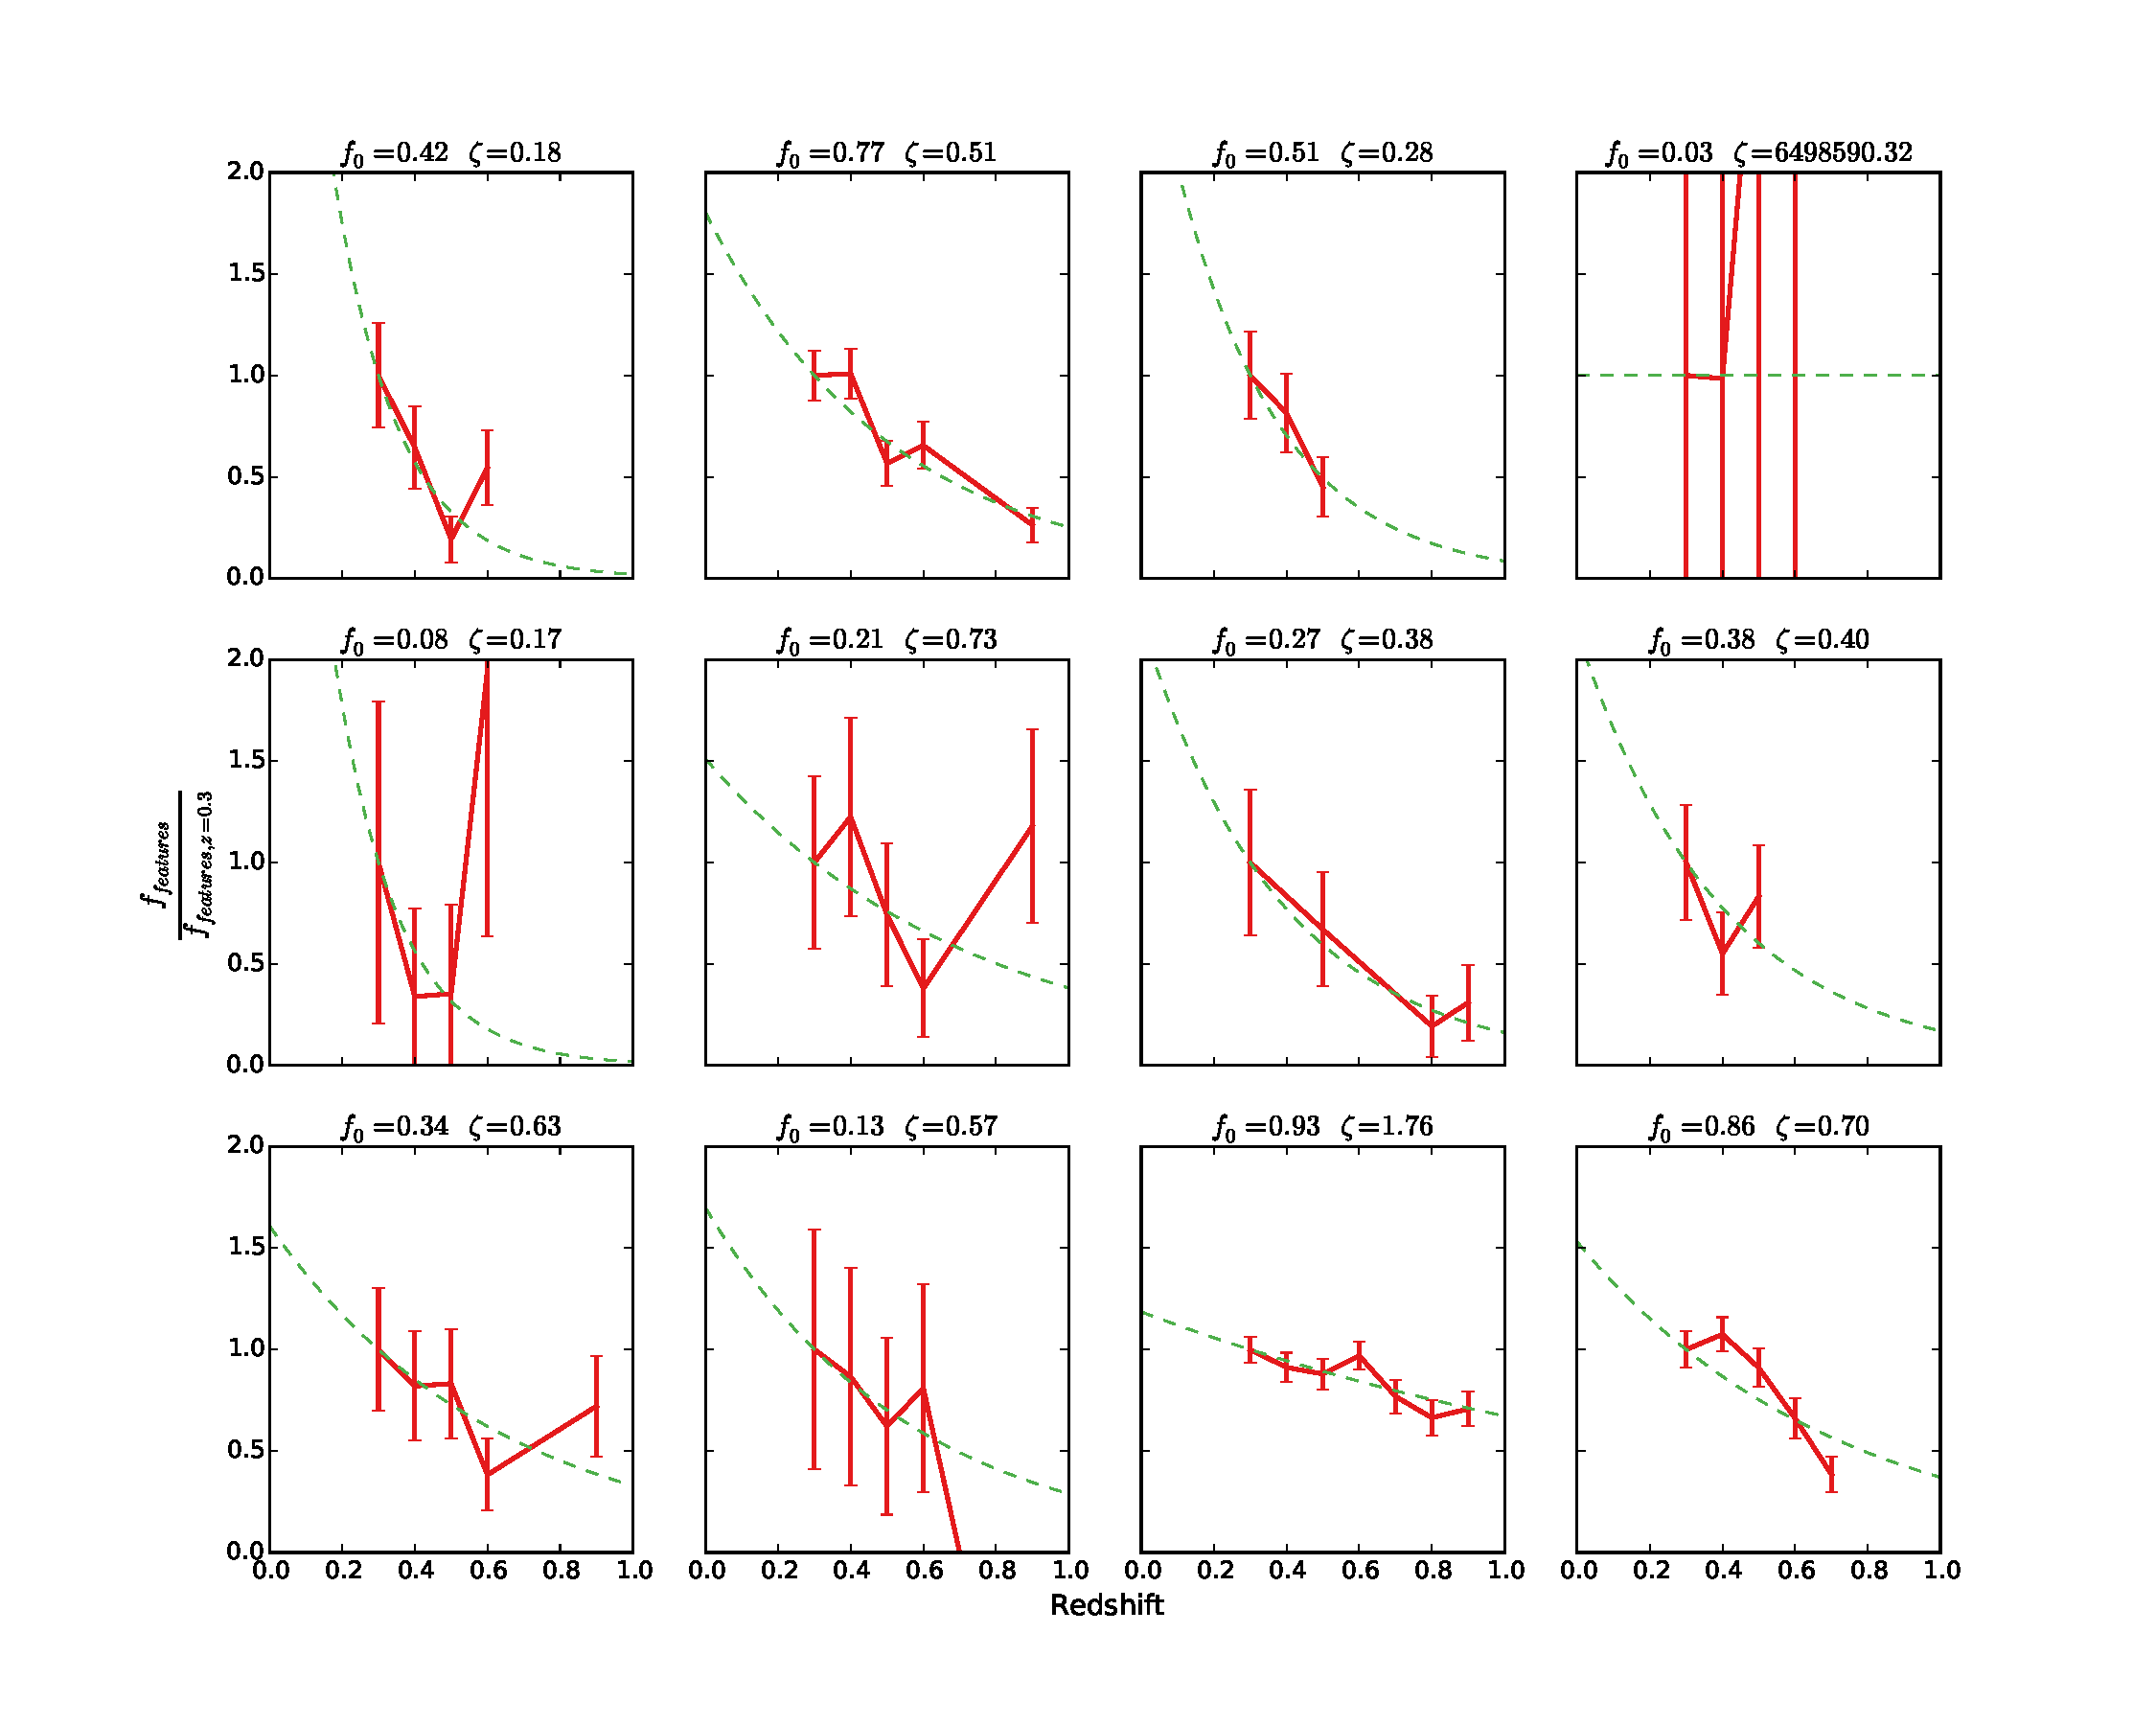
\includegraphics[width=\textwidth]{figures/zeta_examples.pdf}
\caption{Behavior of the normalized, weighted vote fractions of features
visible in a galaxy ($f_\textrm{features}$) as a function of redshift in the
artificial \ferengi{} images. Galaxies in this plot were randomly selected from
a distribution with $e=0$ and at least three detectable images in redshift bins
of $z\ge0.3$. Measured vote fractions (red points) are fit with an exponential
function (Equation~\ref{eqn:fzeta}); the best-fit parameters are given above
each plot. Error bars are Poissonian, assuming a median of 40~votes per
galaxy.}
\label{fig:zeta_examples}
\end{figure*}

GZH uses the values of $\zeta$ for \emph{all} sets of artificially redshifted
galaxies to fit the overall distribution as a function of surface brightness,
since the correction being applied is expected to vary as a function of the
intrinsic galaxy properties. The galaxies that can be used to measure the
calibration are restricted to those with a non-zero $f_\textrm{features}$ at
$z_\mathrm{sim}=0.3$ and with a reasonable fit ($\Delta \chi^2 > 3.0$) to the
exponential model for the measured change in \ffeatures. 

Figure~\ref{fig:zeta_mu} shows the results of fitting the \ferengi{} images
with Equation~\ref{eqn:fzeta}; the correction is only a weak function of
surface brightness ($\mu$). Higher-surface brightness galaxies have stronger
average corrections, likely because these galaxies are more likely to have
larger $f_\textrm{features}$ values at high redshifts. Low surface brightness
galaxies are more likely to begin low and remain low; the bounded nature of the
dropoff (and variance among the individual voters) means that the average
magnitude of $\zeta$ will be lower. 

\begin{figure}
\center
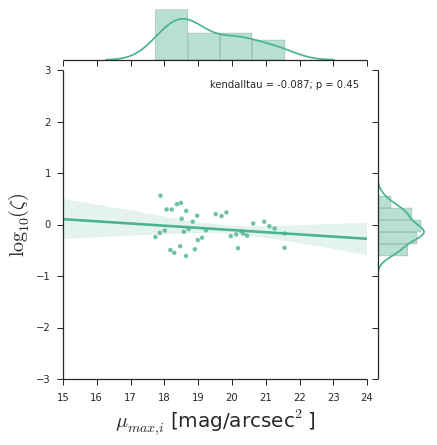
\includegraphics[width=0.50\textwidth]{figures/zeta_mu.png}
\caption{All fits for the vote fraction dropoff parameter $\zeta$ for
\ffeatures{} in the \ferengi{} galaxies as a function of surface
brightness. This includes only those galaxies with a reasonably bounded range
on the dropoff ($-10<\log(\zeta)<10$) and sufficient points to fit each
function (37 original galaxies, each artificially redshifted to create a total
of 296~images}
\label{fig:zeta_mu}
\end{figure}



The data in Figure~\ref{fig:zeta_mu} are fit with a linear function such that:

\begin{equation}
\log_{10}(\hat\zeta) = \zeta_0 + (\zeta_1 \times \mu),
\label{eqn:zetafit}
\end{equation}

\noindent where $\hat\zeta$ is the correction factor applied to each galaxy as
a function of surface brightness. The best-fit parameters to the linear fit
(from least-squares optimization) are $\zeta_0=0.1$, $\zeta_1=1.4$. To make the
final debiased correction, the simple exponential form of
Equation~\ref{eqn:fzeta} is modified to bound the debiased vote fractions
between $f$ and 1:

\begin{equation}
f_\textrm{features,debiased} = 1 - (1 - f_\mathrm{features,weighted})e^{\frac{z-z_0}{\hat\zeta}}.
\label{eqn:fzeta_mod}
\end{equation}

\subsection{Effects of morphological debiasing}\label{ssec:zeta_results}

\begin{figure}
\begin{center}
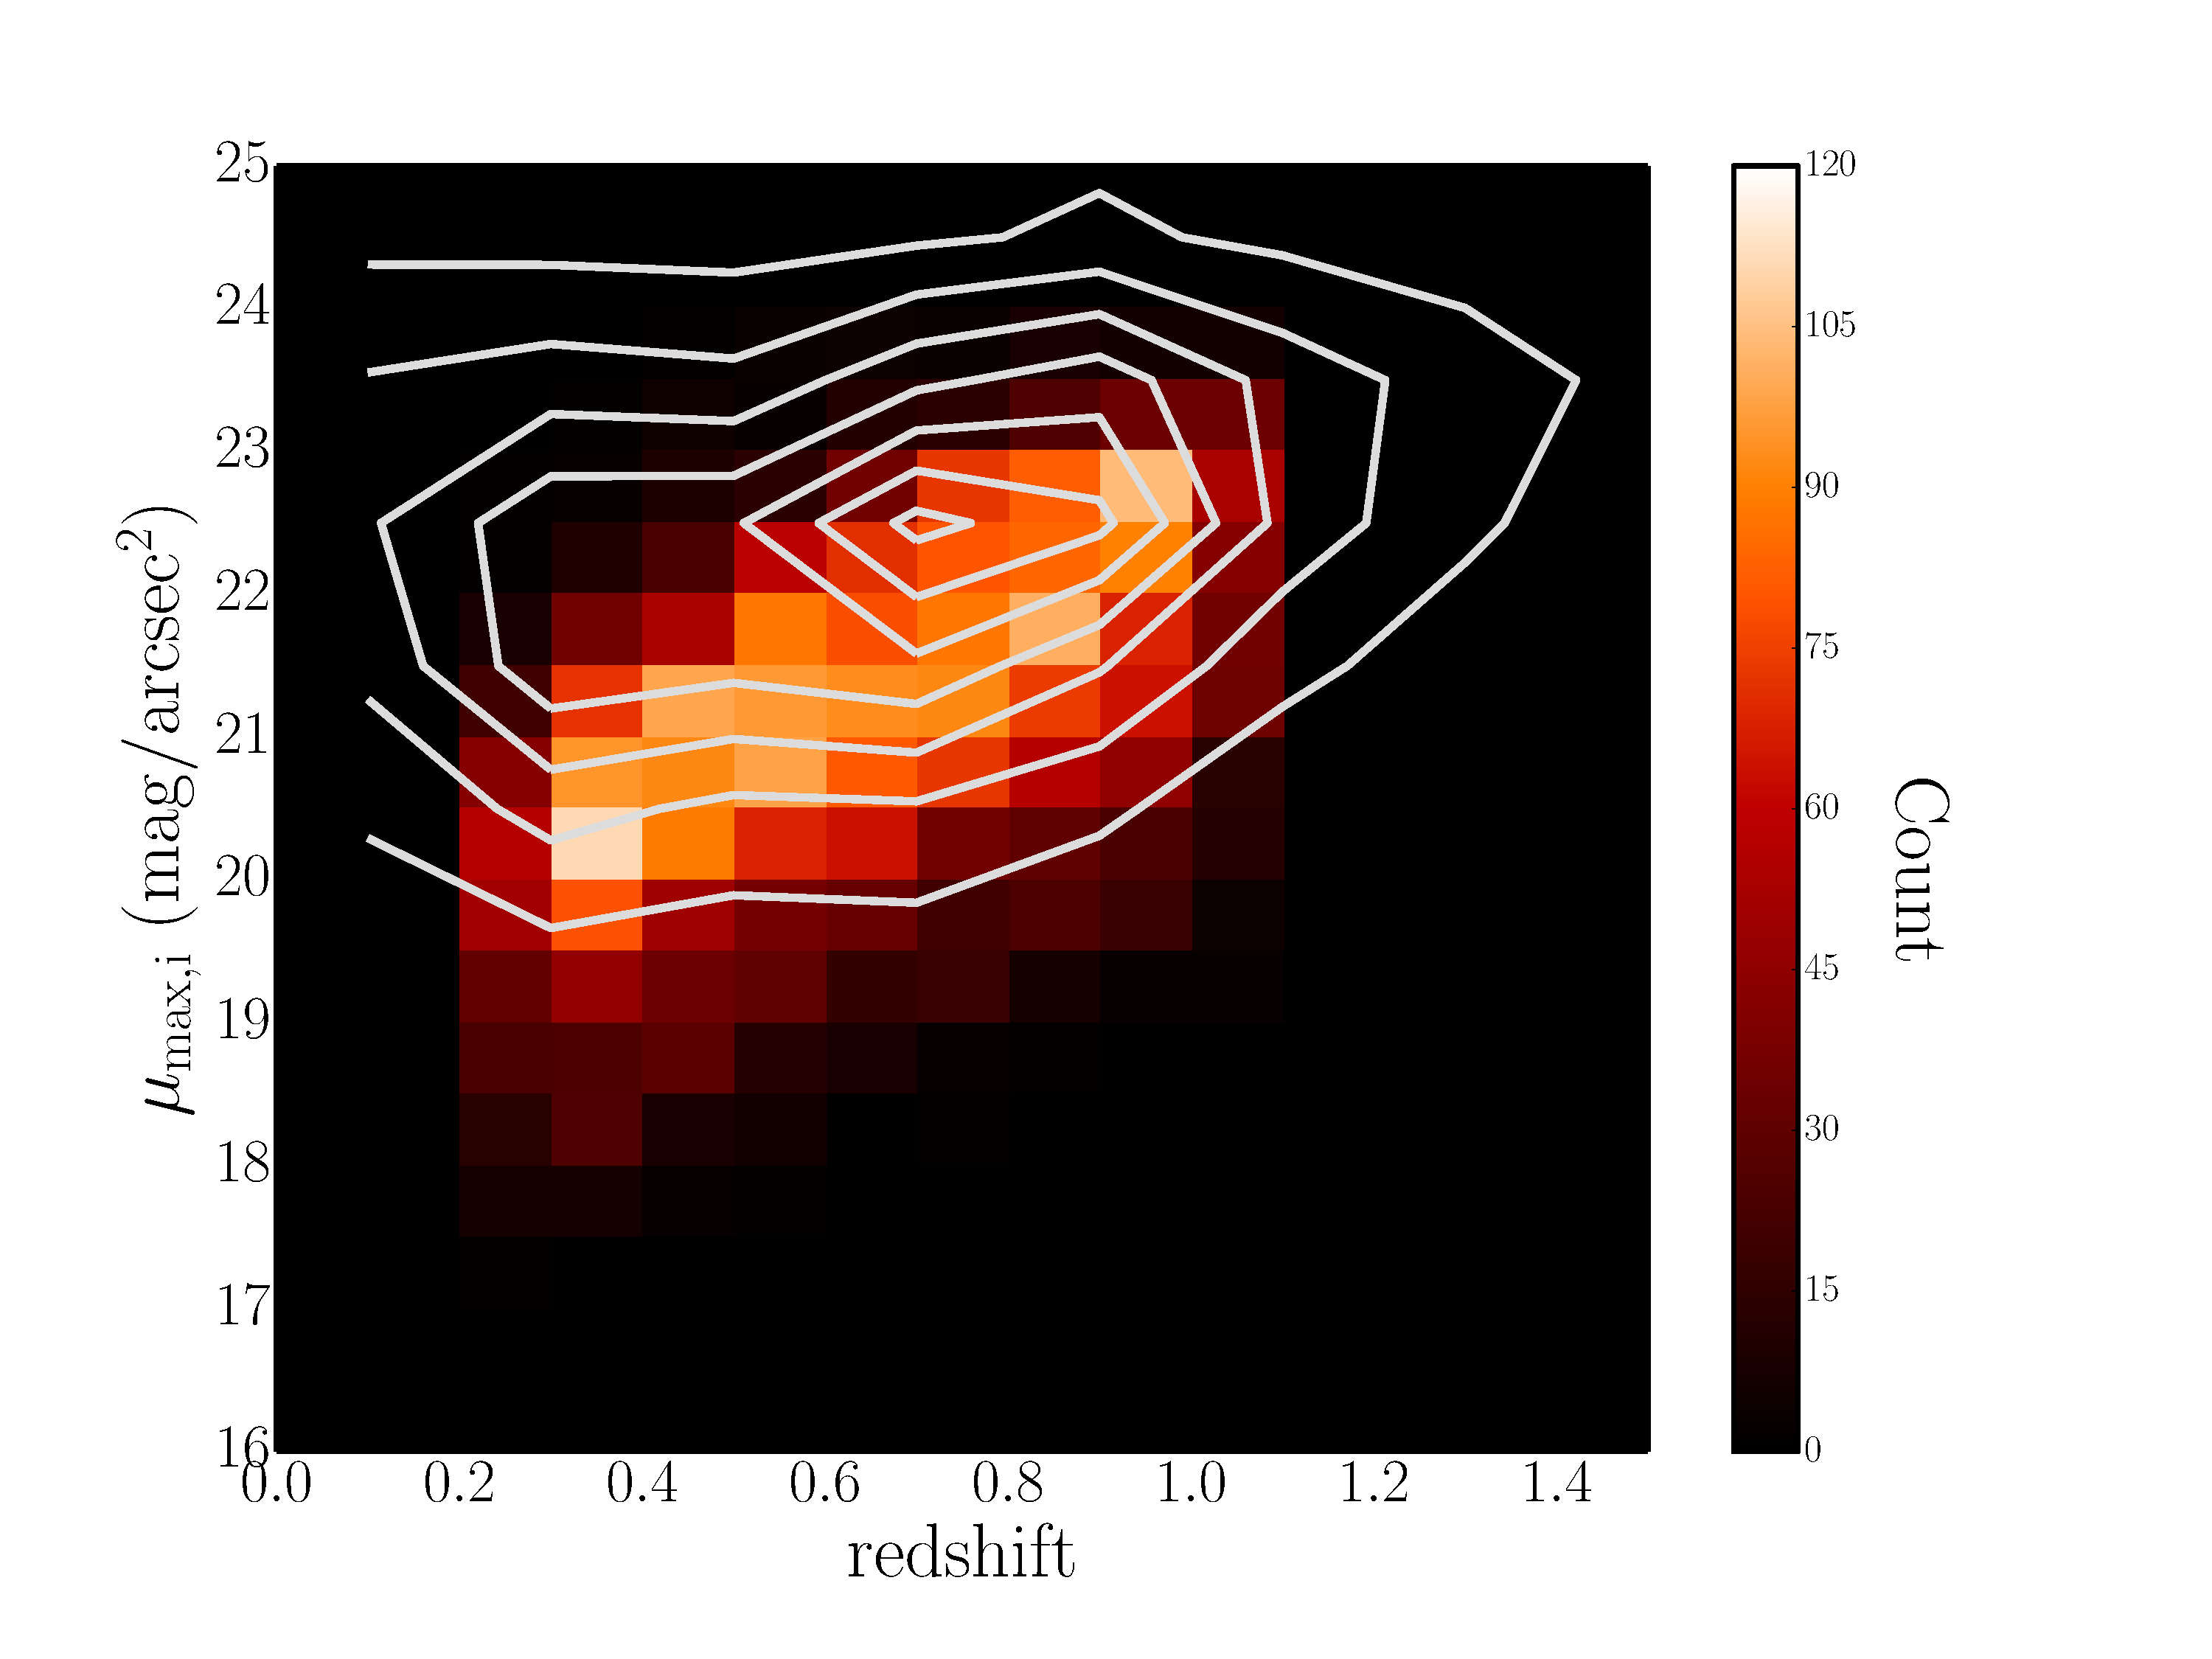
\includegraphics[width=0.5\textwidth]{figures/eye_of_sauron.pdf}
\caption{Surface brightness as a function of redshift for 3,950~\ferengi{}
images and the 102,548~galaxies in the ACS sample with measured $\mu$ and $z$
values. The color histogram shows the number of \ferengi{} images as a function
of $\mu$ and $z_{\rm sim}$. White contours show counts for the full ACS sample,
with contours starting at $N=1000$ and separated by intervals of 1000 up to
7000.} 
\label{fig:sb_redshift}
\end{center}
\end{figure}

\begin{figure*}
\centering
\subfigure{[a]\label{fig:6a}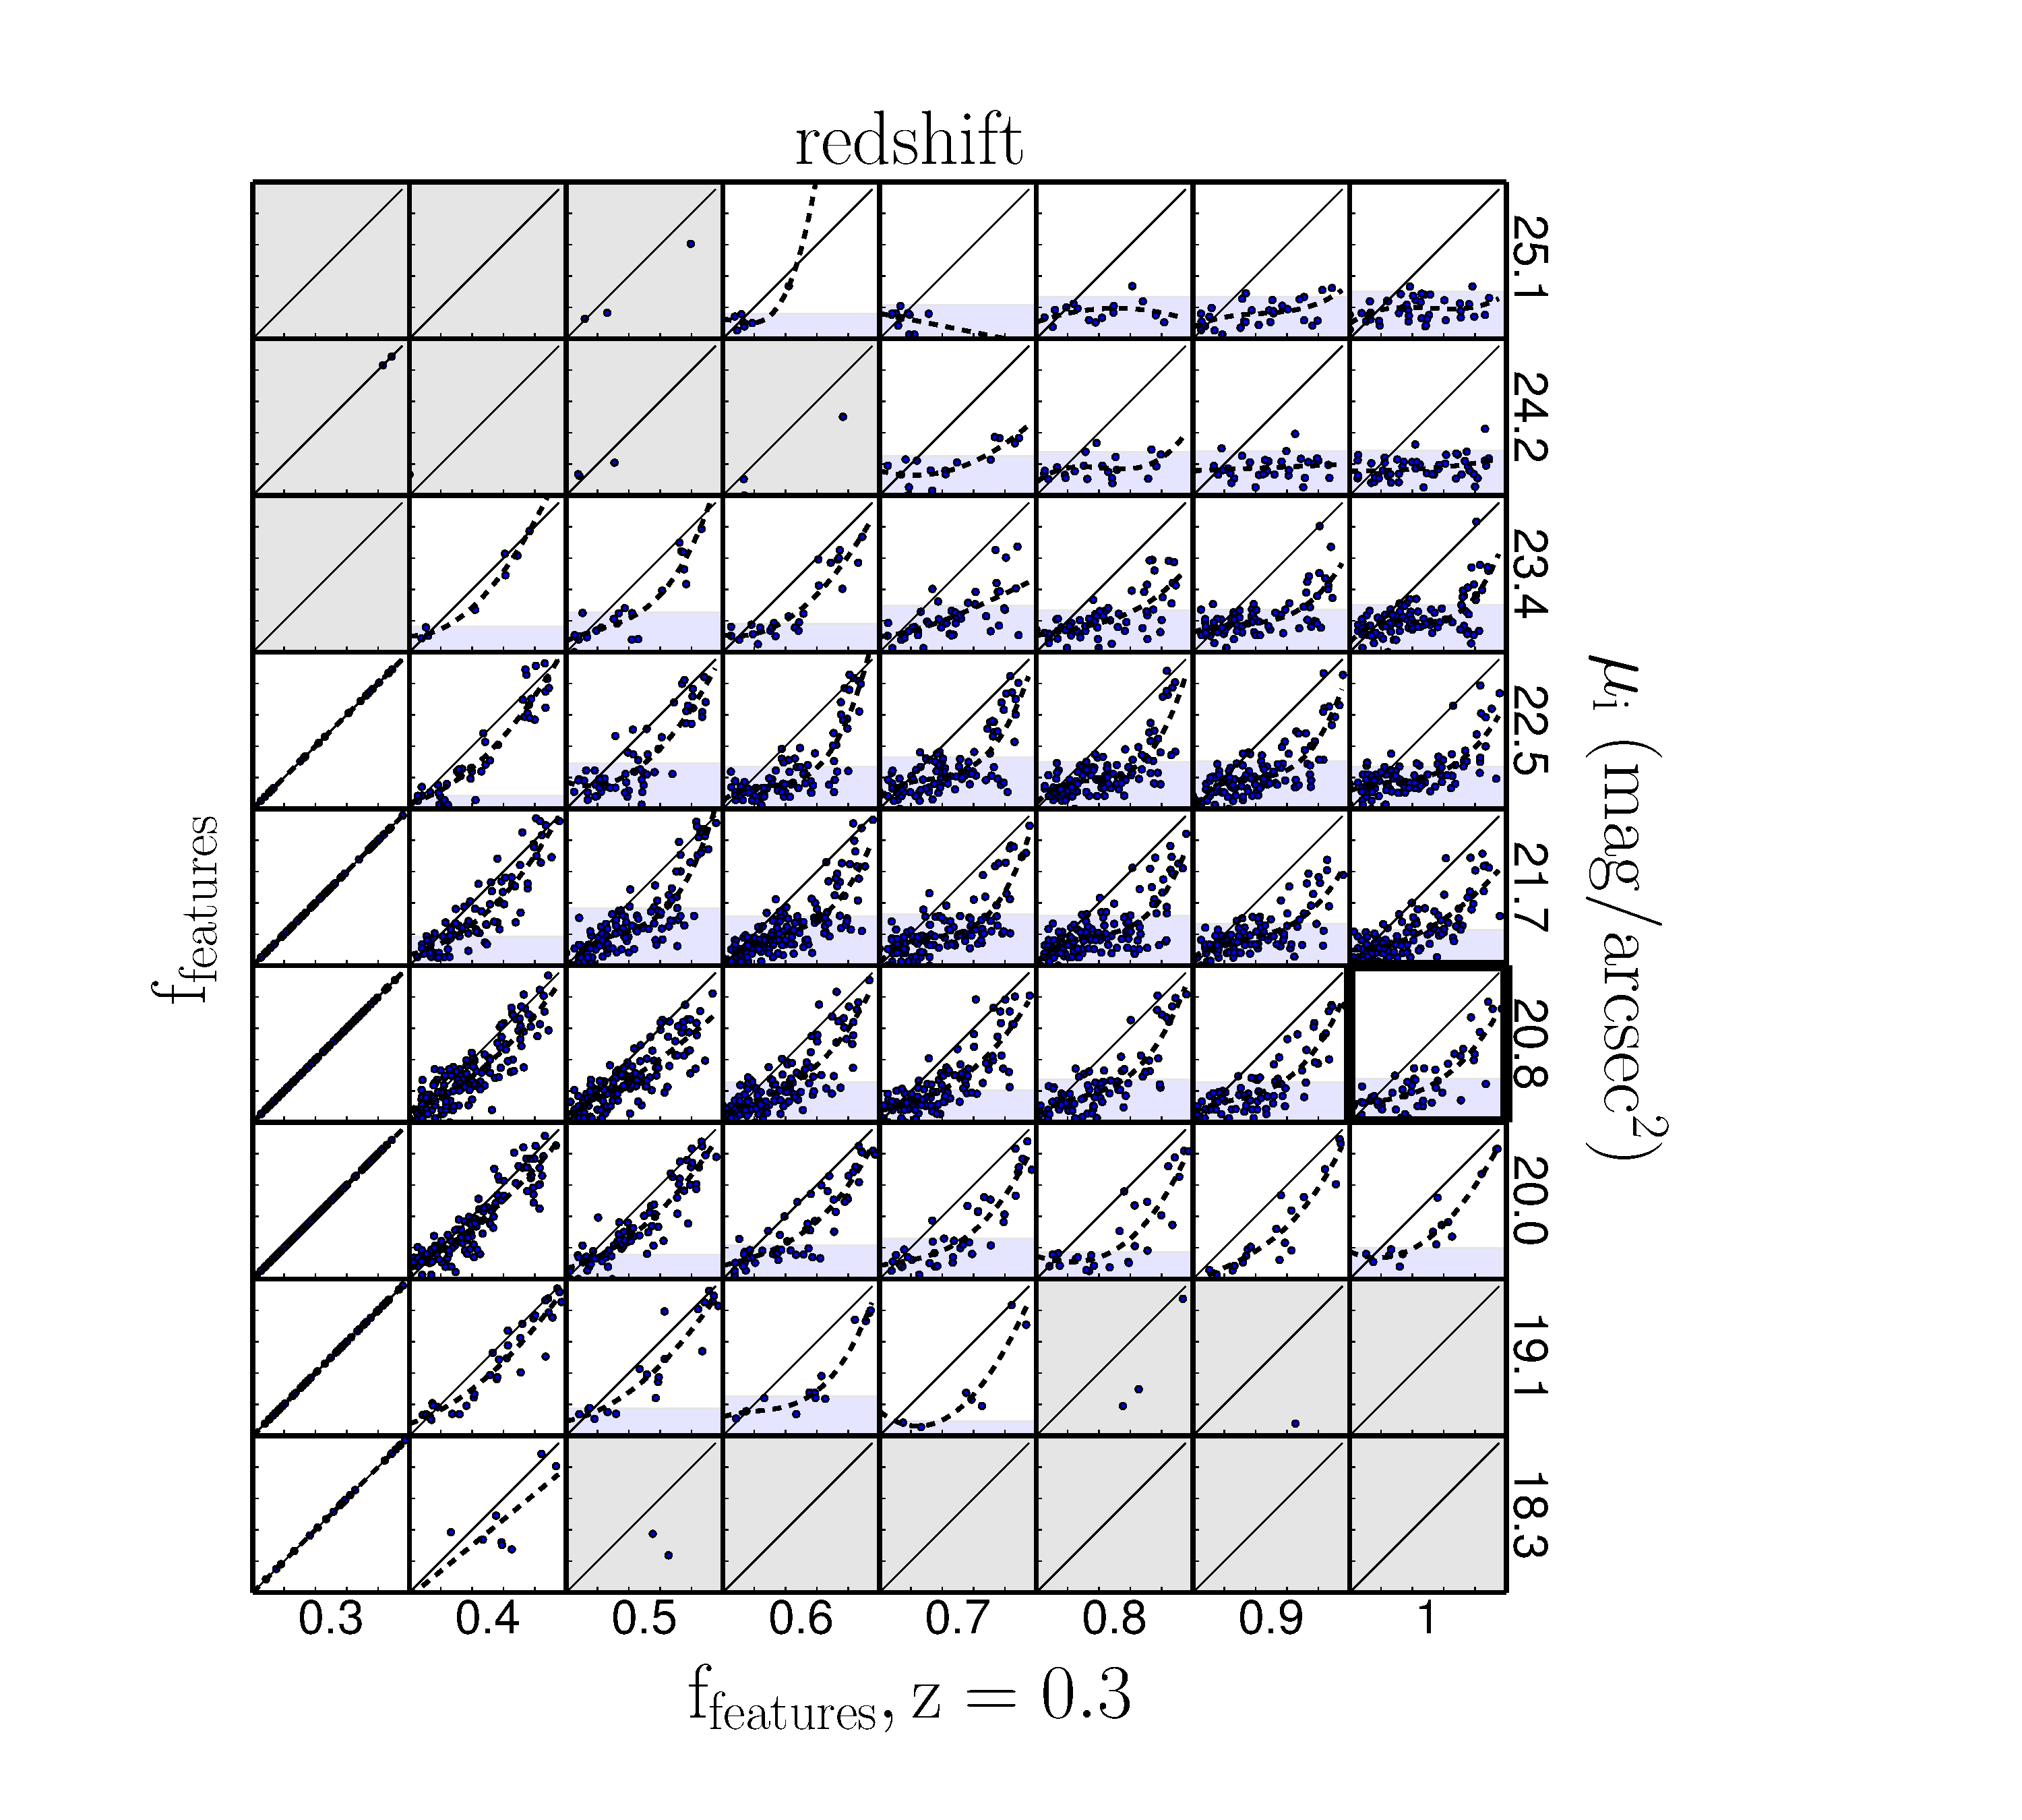
\includegraphics[width=0.5\textwidth]{figures/p_vs_p_SB_redshift.pdf}}
\subfigure{[b]\label{fig:6b}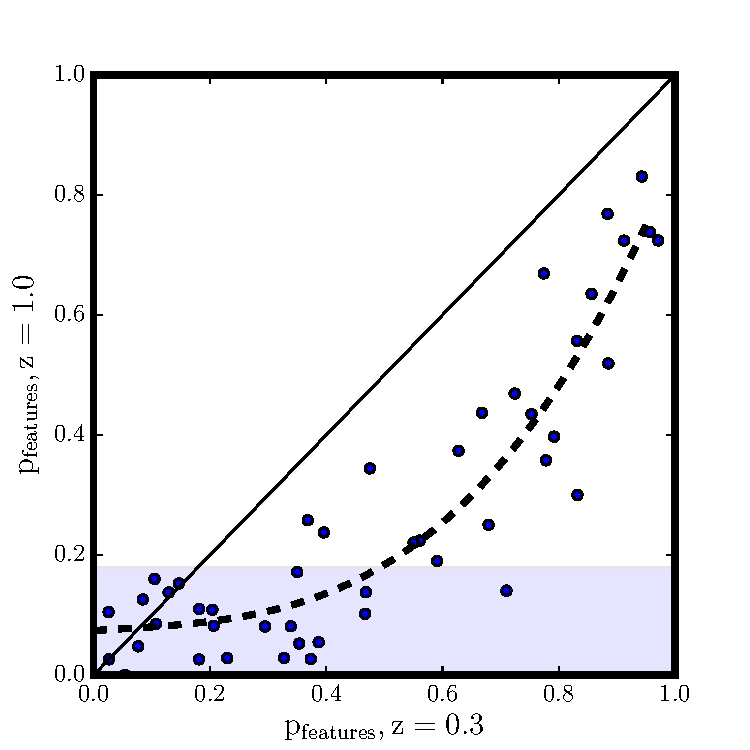
\includegraphics[width=0.4\textwidth]{figures/z1_mu20_subplot1.pdf}}
\\
\subfigure{[c]\label{fig:6c}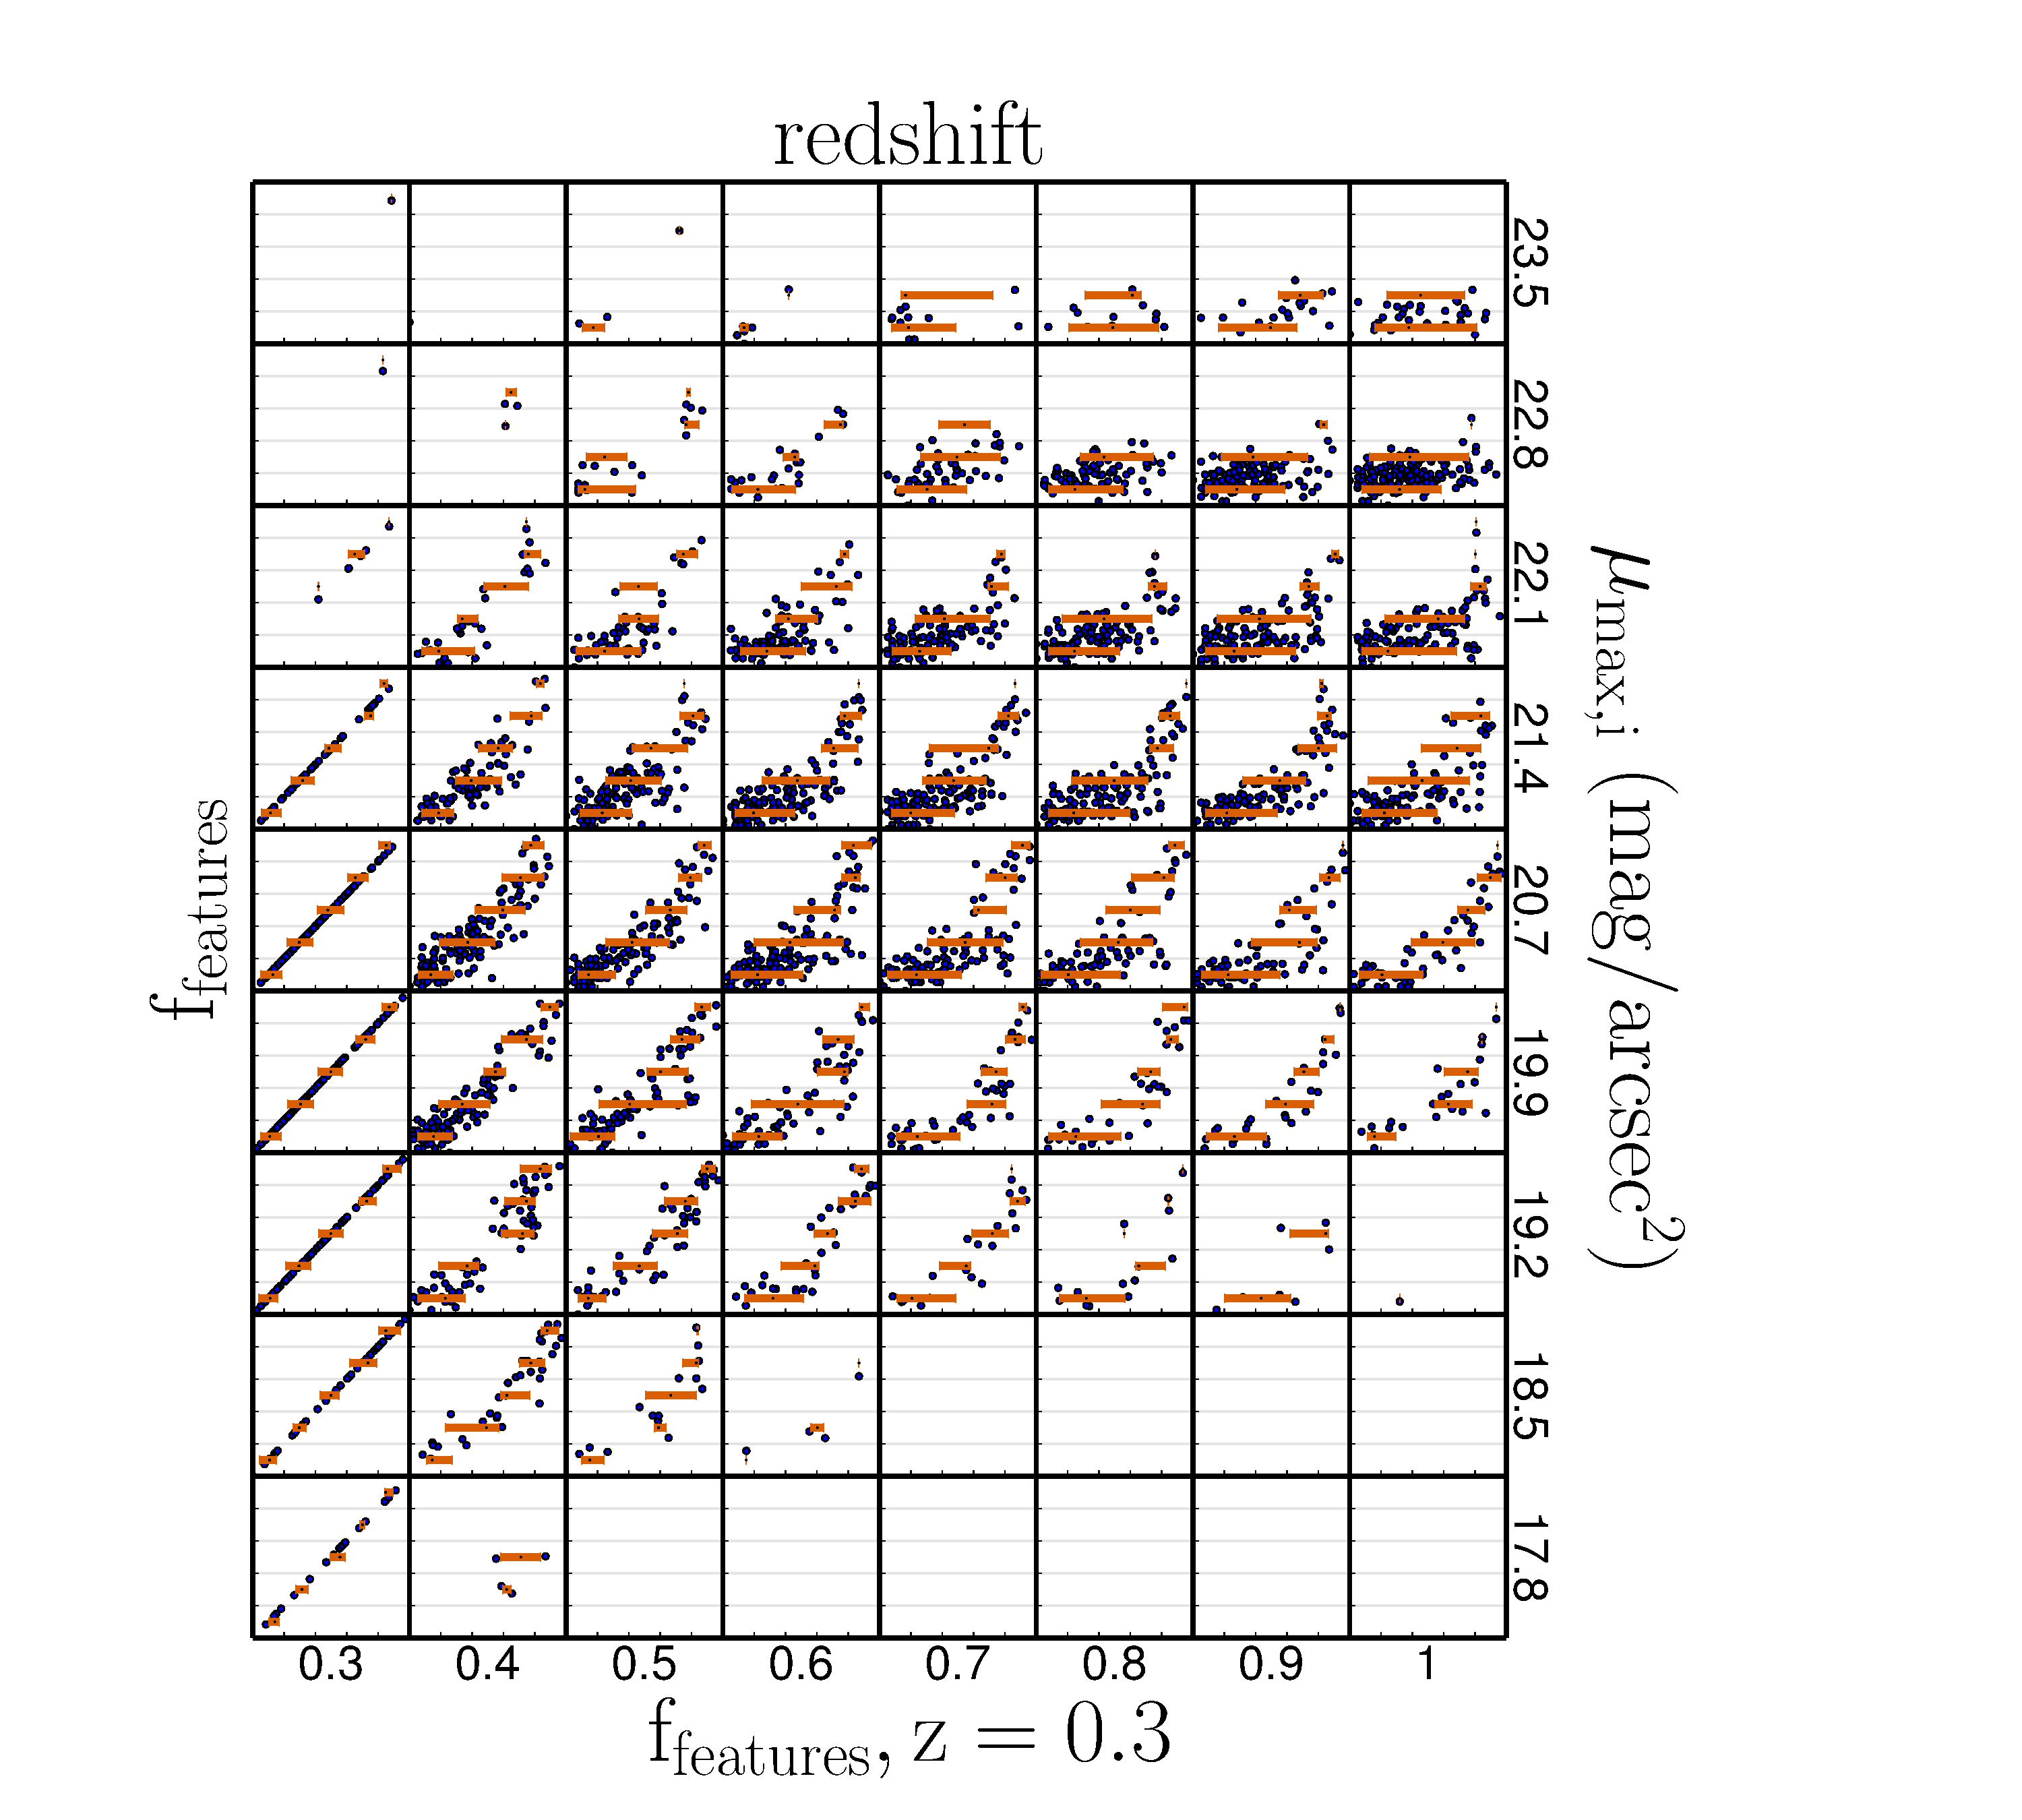
\includegraphics[width=0.5\textwidth]{figures/orangebars.pdf}}
\subfigure{[d]\label{fig:6d}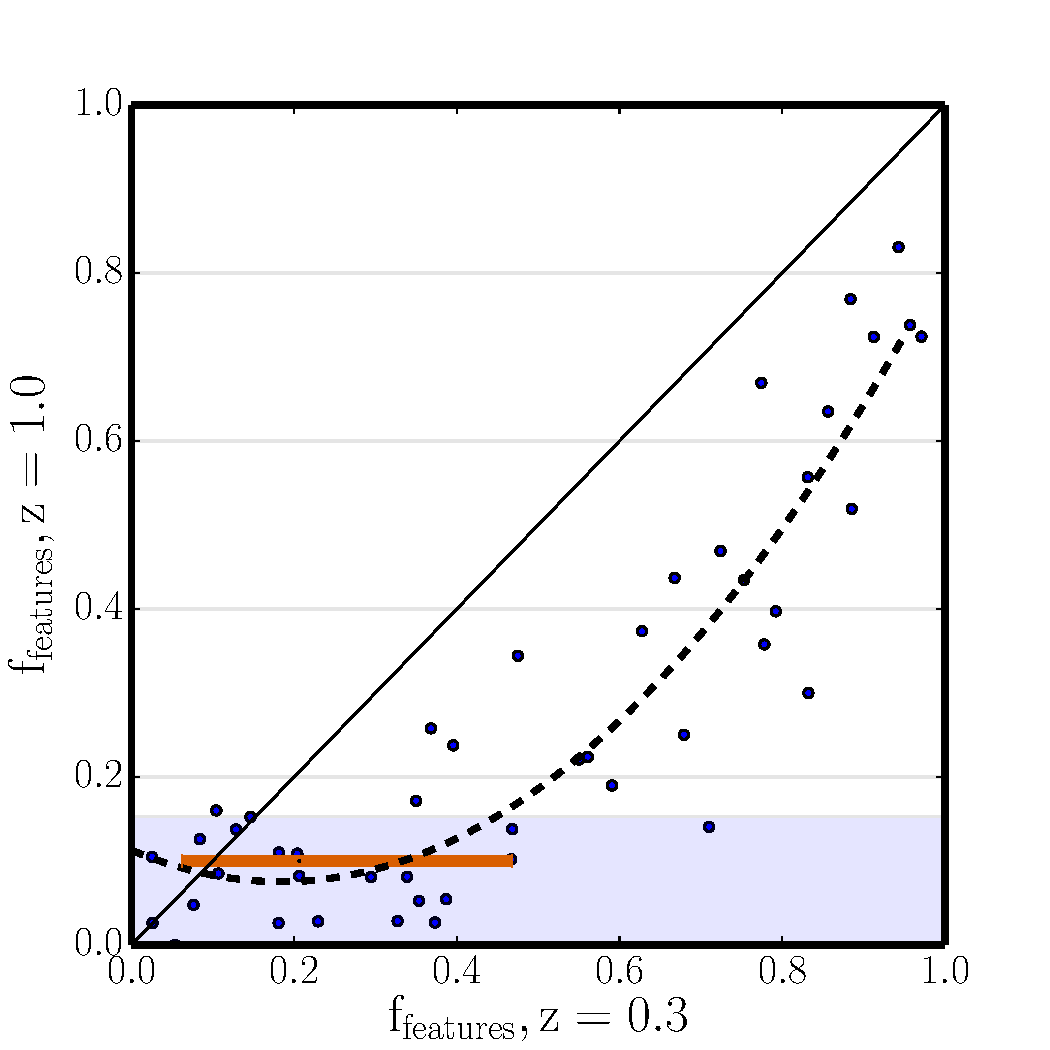
\includegraphics[width=0.4\textwidth]{figures/z1_mu20_subplot2.pdf}}
\caption{Effects of redshift bias in 3,950 images in the \ferengi{} sample.
[a]: Each point in a given redshift and surface brightness bin represents a
unique galaxy. On the $y$-axis in each bin is the \ffeatures{} value of the
image of that galaxy redshifted to the value corresponding to that redshift
bin. On the $x$-axis is the \ffeatures{} value of the image of the same galaxy
redshifted to $z=0.3$. The dashed black lines represent the best-fit
polynomials to the data in each square. The solid black line represents
\ffeaturesz=\ffeaturesrest. Regions in which there is a single-valued
relationship between \ffeatures{} at high redshift and at $z=0.3$ are white;
those in which there is not are blue, and those with not enough data ($N<5$)
are gray. [b]: A larger version of the dark-outlined square in [a], containing
\ferengi{} galaxies that have been artificially redshifted to $z=1.0$ and have
surface brightnesses between $20.3 < \mu < 21.0$ $\rm (mag/arcsec^2)$. [c]: The
same data as [a] is shown. Each $z,\mu$ bin is divided into 4 sub-bins to
determine the range of intrinsic \ffeaturesrest{} for a given range of observed
\ffeaturesz{} values. In each sub-bin, the orange bars represent the inner
80$^\mathrm{th}$ percentiles of the data, the boundaries of which are the lower
and upper limits of the debiased values. [d]: The same data as [b], but
highlighting the upper and lower limit regions.}
\label{fig:f_vs_f}
\end{figure*}

Figure~\ref{fig:f_vs_f} shows the change in \ffeatures{} for the \ferengi{}
galaxies relative to their lowest simulated redshift. In this analysis, only
galaxies whose lowest simulated redshift image was $z_\mathrm{sim}=0.3$ were
used (see Table \ref{tbl:ferengivalues}), and only those which had detectable
surface brightness measurements in \sextractor; this includes 3,950 of the
total 6,466 images. For each simulated redshift value \zsim{} at a fixed
surface brightness $\mu$, \ffeaturesz, the value measured at that simulated
redshift, is plotted against \ffeaturesrest, the value measured for the same
galaxy at \zsim$=0.3$. 
 
The objective is to use these data to predict, for a galaxy with a measured
\ffeaturesz{} value, what its \ffeatures{} value \emph{would have been} if it
had been viewed at $z=0.3$. This predicted value is defined as the debiased
vote fraction \ffeaturesdebiased, and is calculated by applying a correction to
the measured value of \ffeatures, determined by the $\zeta$ function described
in the previous section. A reliable predicted value can be obtained so long as
the relationship between \ffeaturesz{} and \ffeaturesrest{} is single-valued;
that is, for a given \ffeaturesz, there is exactly one corresponding value of
\ffeatures{} at $z=0.3$. 

Figure~\ref{fig:f_vs_f} shows that the relationship between \ffeaturesz{} and
\ffeaturesrest{} is \emph{not} always single valued; hence, it is not
appropriate to correct galaxies that lie in certain regions of surface
brightness/redshift/\ffeatures{} space. These regions tend to have low
\ffeatures{} values at high redshift, but a wide range of values at $z=0.3$.
These regions contain two morphological types of galaxies: the first set are
genuine ellipticals, which have low values of \ffeatures{} at both high and low
redshift. The second group are disks whose features become indistinct at high
redshift; hence their \ffeatures{} value at $z=0.3$ may be quite high, while
the value observed at high redshift is very low. This effect is strongest at
high $z$ and low $\mu$, where features become nearly impossible to discern in
the images.

The criteria for determining whether a region of this space is single-valued,
and therefore correctable, is as follows: In each surface brightness and
redshift bin, the relationship between \ffeaturesz{} and \ffeaturesrest{} is
modeled by fitting the data with a polynomial of degrees $n=3$, 2, and 1, and
using the best formal fit out of the three as measured by the sum of the
residuals. These fits are shown as the dashed black lines in
Figure~\ref{fig:6a}. Any flat regions of the polynomial fits are areas in which
there is not a clear single-valued relationship between \ffeaturesz{} and
\ffeaturesrest; this is quantified by setting a minimum slope cut of 0.4. Any
data in which the polynomial fit has a slope less than this value is considered
\emph{not} one-to-one, and therefore \ffeaturesz{} cannot be boosted to its
\ffeaturesrest{} value.  Galaxies in this region are referred to as the
\emph{lower limit} sample, because the most stringent correction available is
that the weighted \ffeatures{} is a lower limit to the true value.  These
regions are highlighted in blue in Figure~\ref{fig:6a}. Uncolored (white)
regions of the plot have sufficiently high slopes to consider the relationship
as single-valued; galaxies in these regions are considered ``correctable'', and
only these are used in measuring the parameters for the $\zeta$ function
(Section~\ref{ssec:zeta}). Only surface brightness/redshift bins with at least
5 galaxies were considered; regions with fewer than 5 galaxies are considered
to have ``not enough information'' to determine the \ffeaturesz{} and
\ffeaturesrest{} relationship, colored gray in Figure~\ref{fig:6a}.

The unshaded regions in Figure~\ref{fig:6a} define discrete ranges of redshift,
surface brightness, and \ffeatures{} a galaxy must have in order for the
debiased correction to be confidently applied to a galaxy in the GZH sample.
While the appropriate correctable regions were defined discretely, the true
correctable region is assumed to be a smooth function of $z$, $\mu$, and
\ffeatures{}. To define this smooth space, we calculate the shape of the convex
hull that encloses the correctable and lower-limit \ferengi{} galaxies in
$z$-$\mu$-\ffeatures{} space. The boundaries are then adjusted until the
contamination from both groups is minimized. The resulting hulls define the
correctable and lower-limit regions for categorizing the \hst{} galaxies. The
results of this method and final categorization of the \hst{} sample are in
Table~\ref{tbl:hubble_debiasable}. Of the galaxies at redshift higher than
$z=0.3$, 17\% can be debiased using the $\zeta$ method, 27\% cannot be
debiased, and 56\% cannot have the potential for a correction determined, due
either to an unknown redshift or insufficient \ferengi{} images corresponding
to the relevant $z$-$\mu$ values.

For the ``lower-limit'' galaxies for which a single debiased \ffeatures{} value
cannot be confidently assigned, the \emph{range} of debiased values is
estimated using a method visualized in Figure~\ref{fig:6c}. This uses the
\ferengi{} simulated data to analyze the range of intrinsic \ffeaturesrest{}
values for any given observed \ffeatures{} value, again as a function of
surface brightness and redshift. Each $z$,$\mu$ bin, shows the spread of
intrinsic values of \ffeaturesrest{} for four ranges of observed \ffeatures.
The range of intrinsic values is defined as the inner 80\% of the data,
represented by the orange bars in Figure~\ref{fig:6c}. For any galaxy which
cannot be directly debiased by the $\zeta$ method, these ranges are used to
denote the upper and lower limits on the expected values \ffeaturesrest{} as a
function of the observed \ffeatures. 

\begin{table}
\center
\caption{Distribution of \ferengi{} images analyzed in Figure~\ref{fig:f_vs_f}.
Correctable images have a single-valued relationship between their measured
\ffeatures{} values at high and low redshifts (white regions in
Figure~\ref{fig:f_vs_f}). Images with only a lower-limit on \ffeatures{} have a
non single-valued relationship (blue regions). NEI (``not enough information'')
images have undetermined relationships due to a lack of data ($N<5$) in their
corresponding $z$-$\mu$ bins (gray regions).\label{tbl:ferengi_corrections}}
\begin{tabular}{lrr}
\hline \hline
				                   & N       & \% \\
\hline 
Correctable                        & 1,884   & 48\% \\
Lower-limit                        & 1,986   & 50\% \\
NEI                                & 80      &  2\%\\
Total                              & 3,950   & 100\% \\
\hline \hline
\end{tabular}
\end{table}

Few galaxies in the sample have sufficiently high corrections to completely
change them from being confidently smooth to featured following the bias
correction (Figure~\ref{fig:debiased_corrections}). As a check, highly boosted
galaxies are compared to the expert classifications in CANDELS \citep{kar15}.
There are only eight galaxies that were strongly boosted (\ffeatures$<0.2$ and
\fbest$>0.5$) in GZH and also appears in the CANDELS expert sample. Of those
eight galaxies, \citet{kar15} classify 5 as spheroids, 2 as disks, and 1 as
irregular/disky. The \fbest{} values for GZH are all between 0.5 and 0.6,
making them intermediate disk candidates. One of the spheroids has a hint of
extended emission to the south that may have been missed by the CANDELS
experts, but almost all images are dim and with very low surface brightnesses
in the ACS imaging, making positive identification challenging. Since the
surveys use different rest-frame filters and the overlap sample is tiny,
though, detailed comparisons between the overall morphologies are highly
difficult.

\begin{figure*}
\center
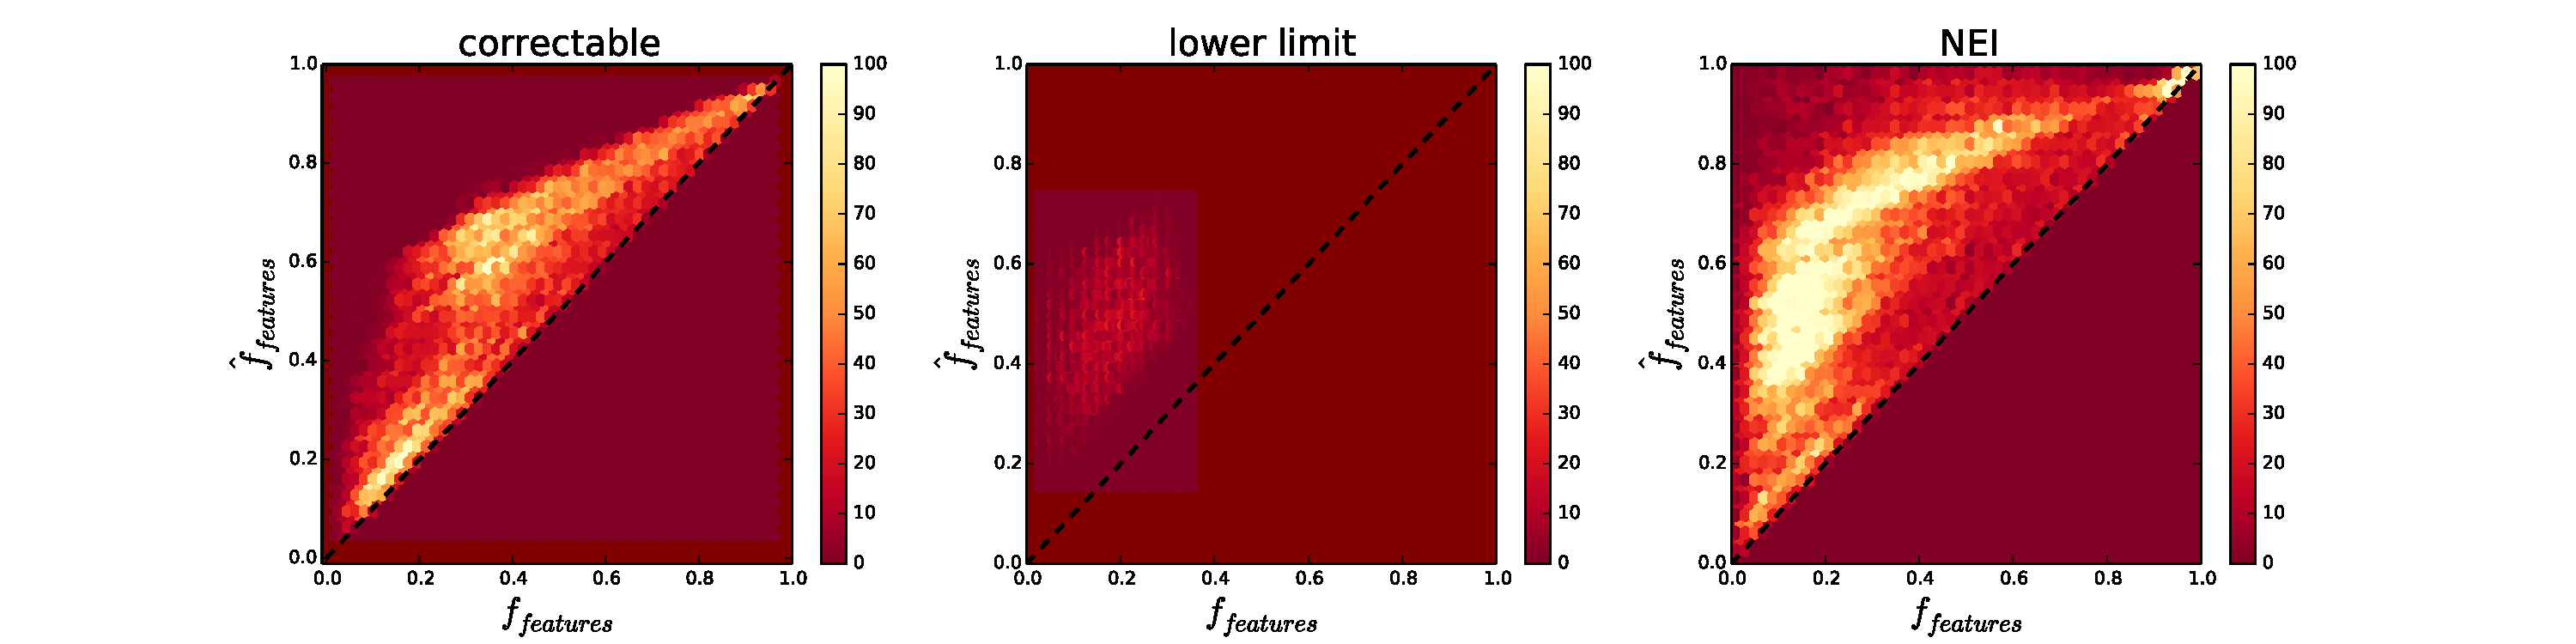
\includegraphics[width=\textwidth]{figures/debiased_corrections.pdf}
\caption{Debiased \ffeatures{} corrected to $z=0.3$ vs weighted \ffeatures{}
for the correctable (left), lower-limit (middle), and NEI (right) galaxies in
    the GZH sample.}
\label{fig:debiased_corrections}
\end{figure*}


\subsection{Challenges of debiasing questions beyond ``smooth or features''}\label{ssec:higher_order_tasks}

As with the HST images, each \ferengi{} subject had a varying number of classifiers
answering the various questions in the hierarchical decision tree. Every classifier
answers the first question, {\it ``Is the galaxy smooth and rounded, with no
sign of a disk?''}; as such the vote fractions \fsmooth, \ffeatures, and
\fartifact{} are all computed with the minimum statistical error for any
question, with between 40 and 140~responses (see Section~\ref{sec:interface}).
The number of participants answering subsequent questions, however, is always equal
to or less than the number who answered the preceding question. The average number
of responses per task for fourth- or fifth-tier questions such as spiral arm
structure (Tasks 12--14) is only $4\pm4$ for the \ferengi{} sample; while this
is distribution is strongly bimodal (reflecting the true morphologies of
selected galaxies), the very low absolute numbers of votes introduce very high
variance when attempting to calculate a statistical correction.

In the \ferengi{} data, these numbers severely limit the amount of information
that can be extracted for the higher-tier questions. The debiasing technique
used (Section~\ref{ssec:zeta}) requires that at least 10~classifiers answer each
question for a galaxy with $z_\mathrm{sim}=0.3$ \emph{and} the corresponding
image at higher redshift. This requirement is (by default) met by all galaxies
for the smooth/features question. However, this is often \emph{not} met for
questions beyond Task~01; on average. $60\%\pm24\%$ of the galaxies do not have
sufficient data to measure a correction, as compared to 2.0\% achieved for
Task~01 (Table~\ref{tbl:ferengi_corrections}). Of the remaining
\ferengi{} galaxies which did meet this requirement, polynomials were fit to
the data in each redshift-surface brightness bin, as was done for Task~01. The
goodness-of-fit was evaluated in each bin, for each Task, using a normalized
$\chi^2$ metric. The mean $\chi^2$ for all higher-order tasks was
$0.10\pm0.04$, significantly larger than the Task~01 value of $0.04$. Based on
this statistic, the data cannot not be modeled with sufficient confidence for
the higher order tasks. An example of the debiasing technique applied to
\fbar{} is shown in Section~\ref{sec:ferengi_bar}; visual inspection of
Figure~\ref{fig:f_vs_fbar} confirms that the points in each bin are scattered
to a degree at which no strong correlation is present.  For these reasons,
debiased vote fractions are only offered in the GZH catalog for Task~01
(smooth/features).  

\begin{table*}
\caption{Correctable fractions for the top-level task in GZH, split by survey.}\label{tbl:hubble_debiasable}
\begin{tabular}{lcrrrrrrr}
\hline\hline
                                   & Correction type & AEGIS   & COSMOS & GEMS & GOODS-N & GOODS-S    & SDSS    & Total \\
\hline
Correctable                        & 0               & 1,654   & 15,170 & 1,837 & 993    & 835     	& 0       & 20,489\\
Lower-limit                        & 1               & 1,917   & 26,113 & 2,423 & 1,385  & 1,282   	& 0       & 33,120\\
No Correction Needed ($z \le 0.3$) & 2               & 955     & 11,926 & 1,175 & 415    & 400     	& 37,545  & 52,416\\ 
NEI                                & 3               & 2,847   & 34,511 & 3,308 & 2,535  & 2,523   	& 0       & 45,724\\
No Redshift Information            & 4               & 1,134   & 5,088  & 561   & 687    & 102   		& 14,316  & 21,888\\
\hline
Total                              &                 & 8,507   & 92,808 & 9,304 & 6,015  & 5,142   	& 51,861  & 173,637\\
\hline\hline
\end{tabular}
\end{table*}

%\begin{figure*}
%\center
%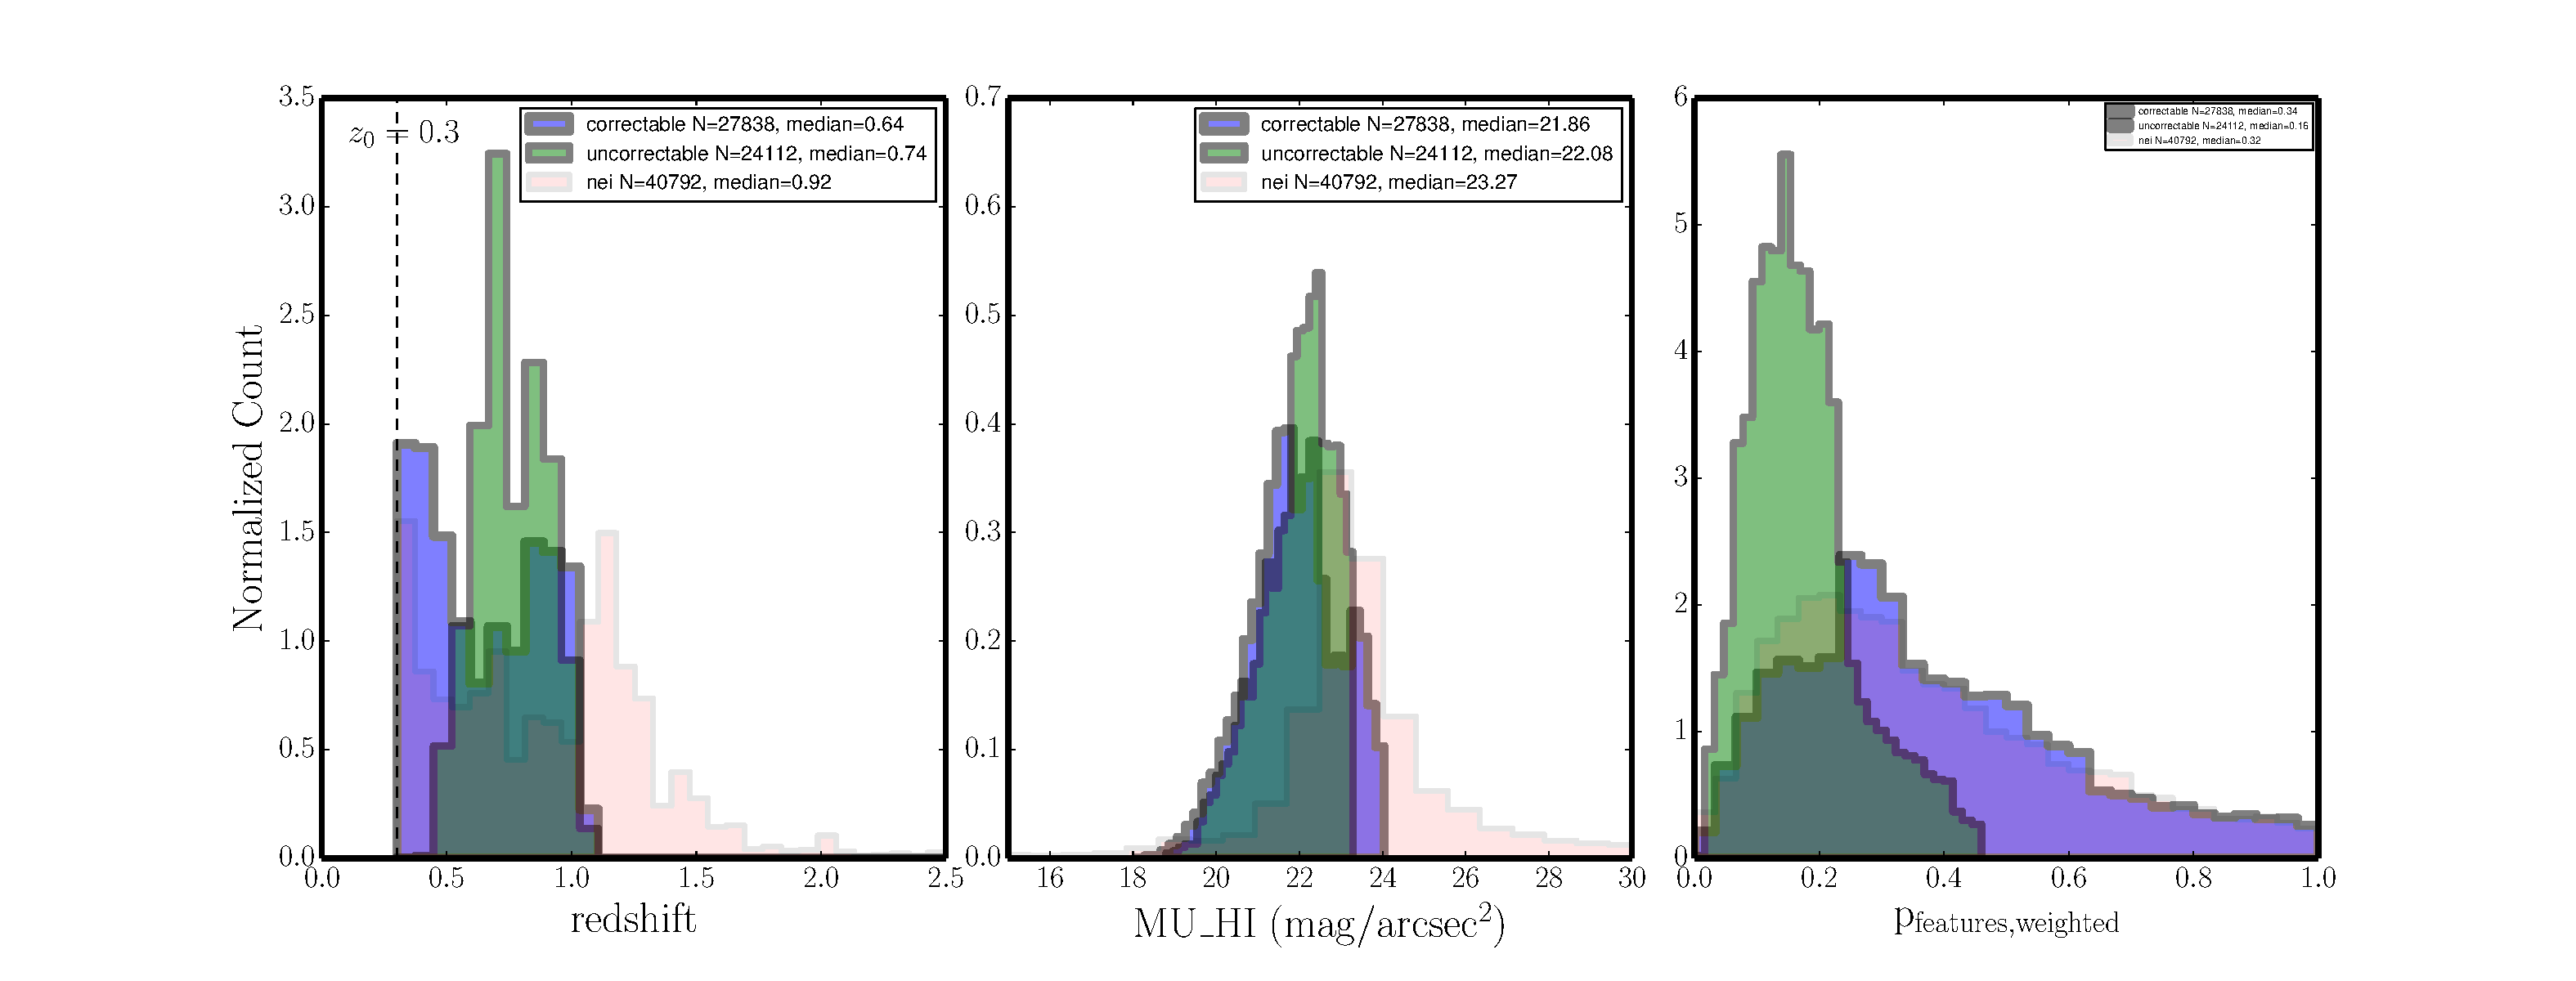
\includegraphics[width=\textwidth]{figures/hubble_z_mu_p_distributions.pdf}
%\caption{Distributions of redshift, surface brightness, and \ffeatures{} for
%correctable (purple), lower-limit (green), and NEI (pink) galaxies in the full
%GZH sample. The lower-limit galaxies have higher redshifts, slightly lower
%surface brightness, and lower values of \ffeatures{} on average than the
%correctable galaxies. The long tail of NEI galaxies in redshift and surface
%brightness demonstrates the limits of the \ferengi{} sample, for which there
%is no data at $z>1$ or $\mu>24$.}
%\label{fig:z_mu_p}
%\end{figure*}


%\subsection{Results of \ferengi{} analysis}
%
%{\bf Old text from Taiwan workshop}
%
%We show here the preliminary results of GZH classifications of images of
%galaxies placed at artificial redshifts. Figure~\ref{fig:ferengi_results_fake}
%shows the range of change of vote fractions for the change of \ffeatures{}
%with redshift, for galaxies with different vote fraction levels, three ranges
%of surface-brightness levels and 7~evolutionary corrections (this last bit is
%indicated by the color). 
%
%%---------------------------------------------------------------------------
%\begin{figure}
%\begin{center}
%
%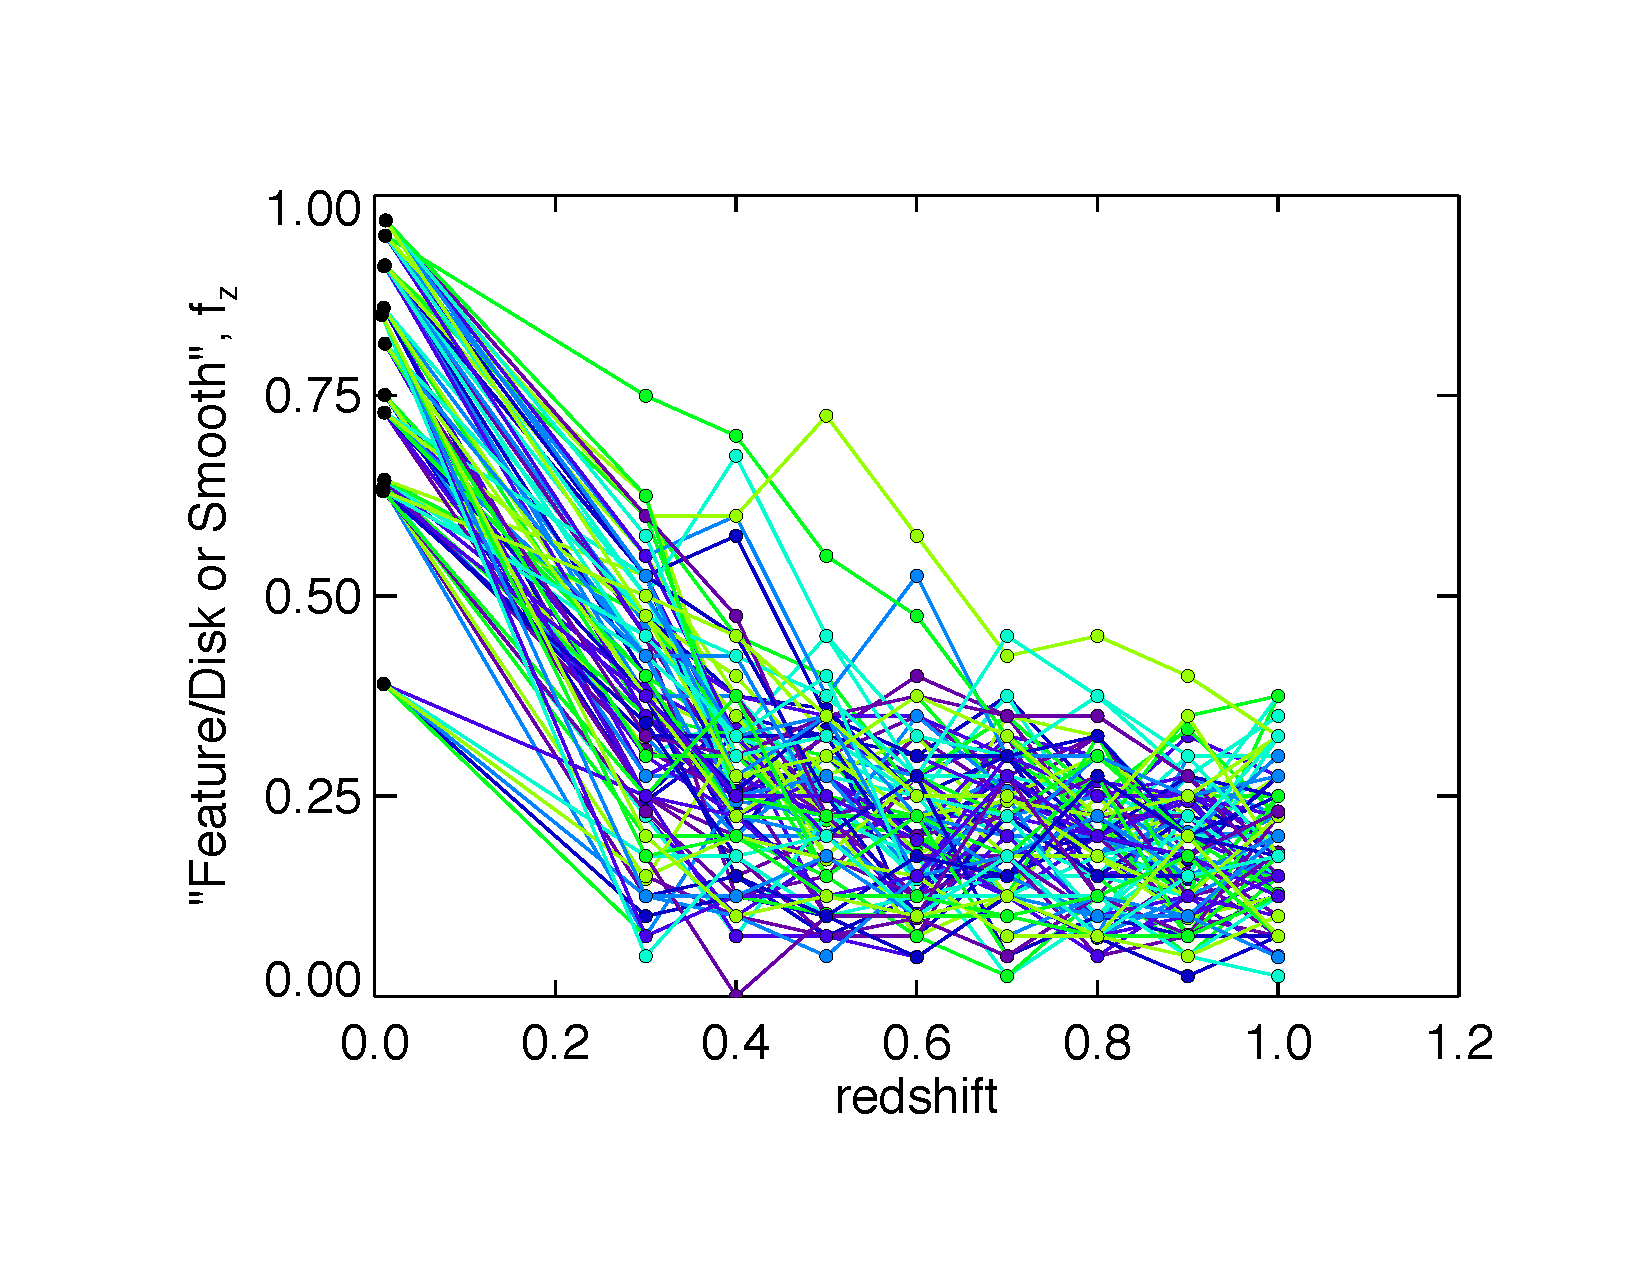
\includegraphics[width=0.45\textwidth]{figures/somewhat_fake_results.pdf}
%
%\caption{Preliminary results of the \ferengi{} redshifting exercise. WARNING
%NO USER WEIGHTING.... For a range of vote fraction levels with three
%surface-brightness levels and 7 evolutionary corrections each (the colors
%indicate evolutionary correction value with green being $e=0$, we show the
%range of evolution of the vote fractions for featured vs. smooth with
%redshift.}
%
%\label{fig:ferengi_results_fake}
%
%\end{center}
%\end{figure}
%%--------------------------------------------------------------------------

\section{The Galaxy Zoo: Hubble catalog}\label{sec:results}

The data release for GZH includes morphological data for 181,101~images
(generated from a total of 150,771~unique galaxies). The full table can be
accessed at \url{http://data.galaxyzoo.org}. The online data also includes a
secondary metadata table, which is drawn from a variety of sources detailed in
Section \ref{sec:data}.

Each image is listed under a unique project ID (eg,~AHZ000001); the actual
galaxy in the image is identified by the combination of the OBJNO and original
survey. For each of the 55~responses in the GZH decision tree, the following
classification data is provided: for each question, $\tt N_{votes}$ is the
number of classifiers who answered that question. For each unique answer, $\tt fraction$
is the fraction of classifiers who selected that answer ($\rm N_{answer}/N_{votes}$, and
$\tt weighted$ is the weighted fraction, which takes into account overall
consistency (Section~\ref{ssec:weighting}). 

The GZH vote fractions can be largely dependent on the resolution of the image.
Two otherwise morphologically identical galaxies which differ significantly in
redshift, brightness, or size may result in very different vote fractions for
any given question, given that many features of a galaxy are difficult to
discern in less-resolved images (bars, spiral arms, disk structure, etc). For
this reason, caution must be used when taking vote fractions as cut-offs to
determine morphological structure; guidelines for careful classification are
given in Section~\ref{sec:cookbook}. 

The GZH catalog is corrected for classification bias only for the first
question of the GZH decision tree (Section~\ref{sec:debiasing}), which asks
{\it ``Is the galaxy smooth and round, with no sign of a disk?''} For this
question, the catalog provides the additional parameters $\tt debiased$, $\tt
lower~limit$, $\tt upper~limit$, and $\tt best$ vote fractions. The $\tt best$
fraction for \ffeatures{} is chosen based on the categorization of the galaxy:
if it is ``correctable'', $\tt best = debiased$; if it is a lower limit, 
$\tt best = lower~limit$; if neither condition applies, then 
$\tt best = weighted$. 

The debiased and best vote fractions for \fsmooth{} are calculated on the
criteria that vote fractions for all answers must sum to unity:

\begin{equation}
f_\mathrm{smooth} \equiv 1 - f_\mathrm{features,best} - f_\mathrm{artifact}.
\label{eqn:constraint}
\end{equation}

\noindent In rare cases ($<1\%$ of the sample), this requirement resulted in
negative vote fractions for \fsmooth; these were cases in which the
\ffeatures{} vote fraction was boosted to a high value relative to \fartifact.
In these cases, the constraint of Equation~\ref{eqn:constraint} is met by
setting \fsmooth$=0.0$ and decreasing \fbest{} accordingly. This correction is
typically small, with a median decrease/increase of
$f_\mathrm{features}/f_\mathrm{smooth}$ of $\Delta f = 0.04$.

Data products for GZH are split by the type of image being classified.
Table~\ref{tbl:catalog_hst} contains the classifications for the \hst{} images
from the AEGIS, COSMOS, and GEMS surveys, as well as 5-epoch deep imaging from
the GOODS-N and GOODS-S surveys. This contains 118,425~galaxies and is the
primary output from the GZH project. The next two tables have data for a small
subset of 3,927~COSMOS~images that were re-processed to study the effect of
color balance on morphological classification. Table~\ref{tbl:catalog_faded}
has images that are desaturated to minimize the color contrast;
Table~\ref{tbl:catalog_recolored} has images with the red and blue color
channels inverted. Table~\ref{tbl:catalog_goods_shallow} contains data for
6,144~galaxies with 2-epoch images from GOODS. These have been mostly
supplanted in the main table with deeper 5-epoch GOODS imaging; however, there
are 1,683~galaxies in the shallower imaging that were not classified in the
deeper mosaics. This data can also be compared to the counterparts in
Table~\ref{tbl:catalog_hst} to study the effect of depth on morphological
classification. Tables~\ref{tbl:stripe82_single} and \ref{tbl:stripe82_coadd}
contain data for the SDSS Stripe~82 single-depth and co-added images,
respectively, that were classified using the GZH interface and decision tree.
Finally, Table~\ref{tbl:simulated_agn} contains classifications for images with
artificial point sources intended to simulate the effect of a bright AGN (see
\citealt{sim14} for an example).


\tabletypesize{\scriptsize}
\begin{deluxetable*}{lllcrllllll|c}
\centering
\tablecolumns{13}
\tablewidth{0pc}
\tablecaption{GZH morphological classifications for \hst{} images from AEGIS, COSMOS, GEMS, and GOODS\label{tbl:catalog_hst}} 
\tabletypesize{\scriptsize}
\tablehead{
 & & & 
\multicolumn{2}{c}{\underline{t01\_smooth\_or\_features\_}} &
\multicolumn{6}{c}{\underline{t01\_smooth\_or\_features\_a01\_smooth\_}} &
\colhead{$\ldots$}
\\
\colhead{Project ID} & 
\colhead{Hubble ID} & 
\colhead{Imaging} & 
\colhead{Correction$^{1}$} & 
\colhead{$N_\mathrm{votes}$} & 
\colhead{fraction} & 
\colhead{weighted} & 
\colhead{debiased} & 
\colhead{best} &
\colhead{lower~limit} & 
\colhead{upper~limit} &
\colhead{}
}
\small
\startdata
AHZ100002g  & 10010842  & AEGIS             & 0        & 127       & 0.118    & 0.128     & 0.085    & 0.085    & 0.226     & 0.226    \\
AHZ100002h  & 10010870  & AEGIS             & 4        & 127       & 0.567    & 0.592     & 0.927    & 0.592    & $-$       & $-$      \\
$\ldots$    \\
AHZ20004kd  & 20014731  & COSMOS            & 3        &  44       & 0.682    & 0.675     & 0.147    & 0.675    & $-$       & $-$      \\
AHZ20004ke  & 20014732  & COSMOS            & 2        &  45       & 0.689    & 0.756     & 0.893    & 0.756    & $-$       & $-$      \\
$\ldots$    \\
AHZ400043g  & 90022729  & GEMS              & 1        & 121       & 0.702    & 0.733     & 0.487    & 0.734    & 0.483     & 0.800    \\
AHZ4000416  & 90022735  & GEMS              & 1        & 127       & 0.646    & 0.698     & 0.508    & 0.698    & 0.171     & 0.727    \\
$\ldots$    \\
AGZ0007z47  & 10014     & GOODS-N-FULLDEPTH & 1        & 40        & 0.475    & 0.475     & 0.197    & 0.475    & 0.011     & 0.496    \\
AGZ0007z48  & 10017     & GOODS-N-FULLDEPTH & 3        & 40        & 0.675    & 0.675     & 0.048    & 0.675    & 0.168     & 0.669    \\
$\ldots$    \\
AGZ00083jb  & 8869      & GOODS-S-FULLDEPTH & 1        & 40        & 0.425    & 0.425     & 0.109    & 0.425    & 0.070     & 0.548    \\
AGZ00083jc  & 8878      & GOODS-S-FULLDEPTH & 0        & 40        & 0.205    & 0.205     & 0.048    & 0.048    & $-$0.005  & 0.287    \\
$\ldots$    \\
\enddata
\tablenotetext{1}{Flag indicating how the vote fractions for this galaxy were
corrected through debiasing (Section~\ref{ssec:zeta_results}), if possible.
0~=~correctable, 1~=~lower-limit ($f_{raw}$ --- $f_{adj}$ is not
single-valued), 2~=~uncorrected ($z_{\rm gal} < 0.3$), 3~=~uncorrected
(insufficient \ferengi{} galaxies in this $z$-$\mu$ bin), 4~=~uncorrected (no
galaxy redshift available).}
\tablecomments{The full version of this table is available in electronic form,
as well as at \url{http://data.galaxyzoo.org}. The complete version includes
data for 118,425~galaxies and morphological information for all tasks in the
tree. A subset of the information is shown here to illustrate form and
content.}
\end{deluxetable*}

% Why are some values negative?
% Why are most of the full-depth GOODS weighted fractions identical to the raw fractions?

\tabletypesize{\scriptsize}
\begin{deluxetable*}{lllcrllllll|c}
\centering
\tablecolumns{13}
\tablewidth{0pc}
\tablecaption{GZH morphological classifications for color-faded Hubble images\label{tbl:catalog_faded}} 
\tabletypesize{\scriptsize}
\tablehead{
 & & & 
\multicolumn{2}{c}{\underline{t01\_smooth\_or\_features\_}} &
\multicolumn{6}{c}{\underline{t01\_smooth\_or\_features\_a01\_smooth\_}} &
\colhead{$\ldots$}
\\
\colhead{Project ID} & 
\colhead{Hubble ID} & 
\colhead{Imaging} & 
\colhead{Correction} & 
\colhead{$N_\mathrm{votes}$} & 
\colhead{fraction} & 
\colhead{weighted} & 
\colhead{debiased} & 
\colhead{best} &
\colhead{lower~limit} & 
\colhead{upper~limit} &
\colhead{}
}
\small
\startdata
AHZF000001  &   20000002    &   COSMOS  &   1   &   48 &  0.708   &     0.755   &   0.228    &    0.754 &   0.325   &   0.829  \\
AHZF000003  &   20000004    &   COSMOS  &   3   &   49 &  0.367   &     0.379   &   0.100    &    0.379 &   0.198   &   0.198  \\
AHZF000004  &   20000006    &   COSMOS  &   3   &   49 &  0.265   &     0.271   &   0.010    &    0.270 &   $-$	    &   $-$    \\
AHZF00000z  &   20000102    &   COSMOS  &   1   &   44 &  0.727   &     0.78    &   0.233    &    0.780 &   0.316   &   0.820  \\
AHZF000010  &   20000104    &   COSMOS  &   2   &   53 &  0.811   &     0.849   &   0.904    &    0.848 &   $-$	    &   $-$    \\
$\ldots$    \\
\enddata
\tablecomments{The full version of this table is available in electronic form,
as well as at \url{http://data.galaxyzoo.org}. The complete version includes
data for 3,927~galaxies and morphological information for all tasks in the
tree. A subset of the information is shown here to illustrate form and
content.}
\end{deluxetable*}

\tabletypesize{\scriptsize}
\begin{deluxetable*}{lllcrllllll|c}
\centering
\tablecolumns{13}
\tablewidth{0pc}
\tablecaption{GZH morphological classifications for color-inverted Hubble images\label{tbl:catalog_recolored}} 
\tabletypesize{\scriptsize}
\tablehead{
 & & & 
\multicolumn{2}{c}{\underline{t01\_smooth\_or\_features\_}} &
\multicolumn{6}{c}{\underline{t01\_smooth\_or\_features\_a01\_smooth\_}} &
\colhead{$\ldots$}
\\
\colhead{Project ID} & 
\colhead{Hubble ID} & 
\colhead{Imaging} & 
\colhead{Correction} & 
\colhead{$N_\mathrm{votes}$} & 
\colhead{fraction} & 
\colhead{weighted} & 
\colhead{debiased} & 
\colhead{best} &
\colhead{lower~limit} & 
\colhead{upper~limit} &
\colhead{}
}
\small
\startdata
AHZC000001	&   20000002	&   COSMOS	&   1	&   168	&   0.615   &   0.664   &   0.160   &  0.663   &  0.271    &  0.775    \\
AHZC000003	&   20000004	&   COSMOS	&   0	&   235	&   0.333   &   0.364   &   0.002   &  0.002   &  0.063    &  0.063    \\
AHZC000004	&   20000006	&   COSMOS	&   3	&   316	&   0.235   &   0.252   & $-0.011$  &  0.252   &  $-$	    &  $-$      \\
AHZC00000z	&   20000102	&   COSMOS	&   1	&   207	&   0.755   &   0.757   &   0.272   &  0.756   &  0.249    &  0.796    \\
AHZC000010	&   20000104	&   COSMOS	&   2	&   158	&   0.843   &   0.882   &   0.936   &  0.881   &  $-$	    &  $-$      \\
$\ldots$    \\
\enddata
\tablecomments{The full version of this table is available in electronic form,
as well as at \url{http://data.galaxyzoo.org}. The complete version includes
data for 3,927~galaxies and morphological information for all tasks in the
tree. A subset of the information is shown here to illustrate form and
content.}
\end{deluxetable*}

\tabletypesize{\scriptsize}
\begin{deluxetable*}{lllcrllllll|c}
\centering
\tablecolumns{13}
\tablewidth{0pc}
\tablecaption{GZH morphological classifications for GOODS 2-epoch images\label{tbl:catalog_goods_shallow}} 
\tabletypesize{\scriptsize}
\tablehead{
 & & &  
\multicolumn{2}{c}{\underline{t01\_smooth\_or\_features\_}} &
\multicolumn{6}{c}{\underline{t01\_smooth\_or\_features\_a01\_smooth\_}} &
\colhead{$\ldots$}
\\
\colhead{Project ID} & 
\colhead{Hubble ID} & 
\colhead{Imaging} & 
\colhead{Correction} & 
\colhead{$N_\mathrm{votes}$} & 
\colhead{fraction} & 
\colhead{weighted} & 
\colhead{debiased} & 
\colhead{best} &
\colhead{lower~limit} & 
\colhead{upper~limit} &
\colhead{}
}
\small
\startdata
AHZ3000001  &   50000000    &     GOODS-N   &   0   &   123	&   0.390   &   0.415	&   0.090 &   0.090 &   $-$     &   $-$      \\
AHZ3000002  &   50000001    &     GOODS-N   &   2   &   126	&   0.341	&   0.355	&   0.356 &   0.356 &   0.220	&   0.279    \\
AHZ3000003  &   50000005    &     GOODS-N   &   1   &   129	&   0.760   &   0.826	&   0.633 &   0.825 &   0.596	&   0.834    \\
AHZ3000004  &   50000008    &     GOODS-N   &   1   &   120	&   0.758	&   0.787	&   0.639 &   0.787 &   0.658	&   0.834    \\
AHZ3000005  &   50000010    &     GOODS-N   &   1   &   123	&   0.854	&   0.890   &   0.611 &   0.889 &   0.597	&   0.914    \\
$\ldots$    \\
\enddata
\tablecomments{The full version of this table is available in electronic form,
as well as at \url{http://data.galaxyzoo.org}. The complete version includes
data for 6,144~galaxies and morphological information for all tasks in the
tree. A subset of the information is shown here to illustrate form and
content.}
\end{deluxetable*}



\tabletypesize{\scriptsize}
\begin{deluxetable*}{lllcrllll|c}
\centering
\tablecolumns{13}
\tablewidth{0pc}
\tablecaption{GZH morphological classifications for SDSS Stripe 82 single-epoch images\label{tbl:stripe82_single}} 
\tabletypesize{\scriptsize}
\tablehead{
 & & & 
\multicolumn{2}{c}{\underline{t01\_smooth\_or\_features\_}} &
\multicolumn{4}{c}{\underline{t01\_smooth\_or\_features\_a01\_smooth\_}} &
\colhead{$\ldots$}
\\
\colhead{Project ID} & 
\colhead{SDSS DR7 ObjID} & 
\colhead{Imaging} & 
\colhead{Correction} & 
\colhead{$N_\mathrm{votes}$} & 
\colhead{fraction} & 
\colhead{weighted} & 
\colhead{debiased} & 
\colhead{best} &
\colhead{}
}
\small
\startdata
AHZ5000001  &   587730845812064684  &   SDSS    &     2 &   41  &   0.585   &    0.595  &   0.759   &   0.594   \\
AHZ5000002  &   587730845812065247  &   SDSS    &     2 &   46  &   0.609   &    0.651  &   0.897   &   0.651   \\
AHZ5000003  &   587730845812196092  &   SDSS    &     2 &   51  &   0.039   &    0.044  &   0.067   &   0.043   \\
AHZ5000004  &   587730845812196825  &   SDSS    &     2 &   35  &   0.514   &    0.605  &   0.928   &   0.605   \\
AHZ5000005  &   587730845812524122  &   SDSS    &     2 &   47  &   0.766   &    0.812  &   1.038   &   0.810   \\
AHZ5000006  &   587730845812654984  &   SDSS    &     2 &   42  &   0.5	    &    0.542  &   0.680   &   0.541   \\
AHZ5000007  &   587730845812655541  &   SDSS    &     2 &   41  &   0.488   &    0.526  &   0.697   &   0.525   \\
AHZ5000008  &   587730845812720365  &   SDSS    &     2 &   53  &   0.792   &    0.84   &   1.050   &   0.839   \\
AHZ5000009  &   587730845812720640  &   SDSS    &     4 &   43  &   0.0	    &    0.0    &   0.0	    &   0.0	    \\
AHZ500000a  &   587730845812720699  &   SDSS    &     2 &   40  &   0.425   &    0.478  &   0.588   &   0.477   \\
$\ldots$    \\
\enddata
\tablecomments{The full version of this table is available in electronic form,
as well as at \url{http://data.galaxyzoo.org}. The complete version includes
data for 21,522~galaxies and morphological information for all tasks in the
tree. A subset of the information is shown here to illustrate form and
content.}
\end{deluxetable*}


\tabletypesize{\scriptsize}
\begin{deluxetable*}{lllcrllll|c}
\centering
\tablecolumns{13}
\tablewidth{0pc}
\tablecaption{GZH morphological classifications for SDSS Stripe 82 co-added images\label{tbl:stripe82_coadd}} 
\tabletypesize{\scriptsize}
\tablehead{
 & & & 
\multicolumn{2}{c}{\underline{t01\_smooth\_or\_features\_}} &
\multicolumn{4}{c}{\underline{t01\_smooth\_or\_features\_a01\_smooth\_}} &
\colhead{$\ldots$}
\\
\colhead{Project ID} & 
\colhead{SDSS DR7 ObjID} & 
\colhead{Imaging} & 
\colhead{Correction} & 
\colhead{$N_\mathrm{votes}$} & 
\colhead{fraction} & 
\colhead{weighted} & 
\colhead{debiased} & 
\colhead{best} &
\colhead{}
}
\small
\startdata
AHZ6000001  & 8647474690312306978   &   SDSS    &    4  & 40  & 0.275   &    0.289  &   0.762   &   0.289   & \\
AHZ6000002  & 8647474690312307154   &   SDSS    &    2  & 43  & 0.605   &    0.634  &   0.858   &   0.635   & \\
AHZ6000003  & 8647474690312307877   &   SDSS    &    2  & 51  & 0.608   &    0.627  &   0.906   &   0.627   & \\
AHZ6000004  & 8647474690312308301   &   SDSS    &    4  & 52  & 0.038   &    0.038  &   0.723   &   0.038   & \\
AHZ6000005  & 8647474690312308318   &   SDSS    &    2  & 44  & 0.614   &    0.632  &   0.776   &   0.631   & \\
AHZ6000006  & 8647474690312308880   &   SDSS    &    2  & 36  & 0.667   &    0.683  &   0.901   &   0.683   & \\
AHZ6000007  & 8647474690312372644   &   SDSS    &    4  & 48  & 0.646   &    0.674  &   1.145   &   0.674   & \\
AHZ6000008  & 8647474690312372789   &   SDSS    &    4  & 45  & 0.489   &    0.571  &   0.964   &   0.570   & \\
AHZ6000009  & 8647474690312372931   &   SDSS    &    4  & 47  & 0.553   &    0.587  &   0.926   &   0.587   & \\
AHZ600000a  & 8647474690312373190   &   SDSS    &    4  & 47  & 0.574   &    0.559  &   1.008   &   0.559   & \\
$\ldots$    \\
\enddata
\tablecomments{The full version of this table is available in electronic form,
as well as at \url{http://data.galaxyzoo.org}. The complete version includes
data for 30,339~galaxies and morphological information for all tasks in the
tree. A subset of the information is shown here to illustrate form and
content.}
\end{deluxetable*}

\tabletypesize{\scriptsize}
\begin{deluxetable*}{lllccccrrrrrrr|c}
\centering
\tablecolumns{14}
\tablewidth{0pc}
\tablecaption{GZH morphological classifications for \hst{} images with simulated AGN\label{tbl:simulated_agn}} 
\tabletypesize{\scriptsize}
\tablehead{
 & & & & & & & &
\multicolumn{6}{c}{\underline{t01\_smooth\_or\_features\_a01\_smooth\_}} &
\colhead{$\ldots$}
\\
\colhead{Project ID} & 
\colhead{SDSS DR7 ObjID} & 
\colhead{Imaging} & 
\colhead{Correction} & 
\colhead{Version} & 
\colhead{$L_\mathrm{ratio}$} & 
\colhead{AGN color$^{1}$} & 
\colhead{$N_\mathrm{votes}$} & 
\colhead{fraction} & 
\colhead{weighted} & 
\colhead{debiased} & 
\colhead{best} &
\colhead{lower limit} &
\colhead{upper limit} &
\colhead{}
}
\small
\startdata
AHZ7000001  &   90024700  &   GEMS    &   1   &   1   &   0.2	    &   1   &   42	&   0.238   &   0.239   &   $-$0.110  &       0.238  &  $-$0.113    &     0.287  \\
AHZ7000002  &   90024700  &   GEMS    &   1   &   1   &   1.0	    &   1   &   51	&   0.255   &   0.265   &   $-$0.107  &       0.264  &  $-$0.128    &     0.272  \\
AHZ7000003  &   90024700  &   GEMS    &   0   &   1   &   5.0	    &   1   &   47	&   0.170   &   0.167   &   $-$0.018  &    $-$0.018  &  $-$0.049    &     0.033  \\
AHZ7000004  &   90024700  &   GEMS    &   0   &   1   &   10.0    &   1   &   41	&   0.195   &   0.195   &      0.045  &       0.045  &     0.044    &     0.127  \\
AHZ7000005  &   90024700  &   GEMS    &   0   &   1   &   50.0    &   1   &   47	&   0.170   &   0.178   &      0.067  &       0.067  &     0.146    &     0.167  \\
$\ldots$    \\
AHZ700013m  &   90024700  &   GEMS    &   0   &   2   &   0.0	    &   0   &   35	&   0.171   &   0.136   &      0.011  &       0.011  &     0.029    &      0.112 \\
AHZ700013n  &   90024700  &   GEMS    &   1   &   2   &   0.2	    &   1   &   20	&   0.150   &   0.158   &   $-$0.278  &       0.049  &  $-$0.351    &      0.049 \\
AHZ700013o  &   90024700  &   GEMS    &   1   &   2   &   1.0	    &   1   &   32	&   0.281   &   0.300   &   $-$0.086  &       0.281  &  $-$0.119    &      0.281 \\
AHZ700013p  &   90024700  &   GEMS    &   0   &   2   &   5.0	    &   1   &   29	&   0.103   &   0.115   &   $-$0.098  &    $-$0.098  &  $-$0.152    &   $-$0.069 \\
AHZ700013q  &   90024700  &   GEMS    &   0   &   2   &   10.0    &   1   &   35	&   0.171   &   0.181   &      0.027  &       0.027  &     0.023    &      0.106 \\
AHZ700013r  &   90024700  &   GEMS    &   0   &   2   &   50.0    &   1   &   34	&   0.206   &   0.206   &   $-$0.005  &    $-$0.005  &  $-$0.056    &      0.026 \\
$\ldots$    \\
\enddata
\tablenotetext{1}{Flag indicating the color of the PSF in the simulated AGN. 0~=~no simulated AGN, 1~=~blue, 2~=~flat, 3~=~red.}
\tablecomments{The full version of this table is available in electronic form,
as well as at \url{http://data.galaxyzoo.org}. The complete version includes
data for 2,961~galaxies and morphological information for all tasks in the
tree. A subset of the information is shown here to illustrate form and
content.}
\end{deluxetable*}

\section{Using the catalog}\label{sec:cookbook}

The intended purpose of the GZH catalog is to provide a simple, yet flexible,
means of identifying samples of galaxies with a desired morphological type.
This section provides instructions for creating such samples using the vote
fractions corresponding to the tasks shown in Figure~\ref{fig:decisiontree}. We
stress that the selection process will vary based on the particular science
case. More conservative cuts can be applied to create pure, but not necessarily
complete, samples. These are useful for selecting galaxies exhibiting unique
morphologies for individual case studies or observing proposals. Looser cuts
can be applied to obtain samples with a higher level of completeness, which
will increase the sample size but can potentially decrease purity. Population
studies would make use of such large samples, in which statistical significance
is a crucial factor in evaluating results. \citet{mas11c,mel14,che15}, and
\citet{gal15} are examples of GZ papers which select morphologies in this way. 

In GZH, participants answered questions about a galaxy's morphology in a decision
tree format. With this structure, questions shown to a classifier were dependent on
their answers to the previous questions (Section~\ref{ssec:interface}).
Figure~\ref{fig:decisiontree} shows the possible paths available for answering
the questions offered in GZH. The colors represent the tier level of Tasks,
which indicate the number of previous Tasks the given Task is dependent upon.
The arm-number question, Task~11, is a 5$^\mathrm{th}$-tier Task, meaning that
whether this question is seen by a classifier was dependent on four Tasks preceding
it. In this case, it as only shown to classifiers who identified the galaxy as
featured/disk-shaped in Task~01, not clumpy in Task~12, not edge-on in Task~02,
and having spiral structure in Task~10.  

To select galaxies of a morphological type identified with a particular Task, a
cut is placed on the vote fraction for that Task ($f_{\rm task}$), \emph{as
well as} the vote fractions for the Tasks preceding it, because of the
dependency induced by the decision-tree structure. For example, to select
barred galaxies, a cut may be placed on \fbar{} such that only galaxies where a
high fraction of votes for this task voted for the $bar,yes$ answer. This is
not the only necessary cut, however, since not all classifiers answer this question;
only those who have previously selected ``features'' in Task~01, ``not clumpy''
in Task~12, and ``not edge-on'' in Task~02 will have the opportunity to vote on
the bar question, Task~03. To ensure that \fbar{} is well-sampled, cuts on all
previous tasks must be applied. 

The flexibility of this catalog allows users to set their own selection
criteria for vote fraction thresholds to create a morphologically pure sample.
Table~\ref{tbl:thresholds} provides baseline cuts for selecting galaxies of a
variety of morphologies. These thresholds are determined by a visual inspection
of subsamples. For each Task, at least 20 classifiers are required to have voted on
the given question along with a cut on the vote fraction is applied to the
previous task. We visually analyzed subsamples of 50~galaxies meeting both
criteria, as well as a control sample of galaxies which had 20~classifiers vote on
the task, but did not meet the threshold cut set for the previous task. The
threshold cut was adjusted and new subsamples were inspected until both the
original and control samples achieved $>80\%$ purity.

As an example of how to use Table~\ref{tbl:thresholds} to create a sample of
3-armed spirals galaxies, we suggest selecting objects with $N_{arm~number} \ge
20$, \ffeatures$>0.23, f_{\rm clumpy,no} > 0.30, f_{edgeon,no}>0.25$, and
$f_{spiral,yes}>0.25$. These cuts define a sample of galaxies of ``arm number
candidates''; \ie, galaxies for which answering the arm number question makes
physical sense and the vote fraction $f_{\rm arm~number}$ is well-sampled. In
this example, such galaxies are featured, non-clumpy, non-edge~on spirals. At
this point a cut can be made on $f_{\rm arm~number=3}$ to select spirals with
three arms. 

Tasks 03, 04 and 05 have an additional possible pathway; as shown in
Figure~\ref{fig:decisiontree}, a classifier might also be shown this question if they
select ``featured/disk'' in Task~01, ``clumpy'' in Task~12, two or more clumps
in Task~16, and ``spiral arrangement'' in Task~15. After applying the
appropriate thresholds for this path, $< 0.5\%$ of the galaxies which have $\ge
20$ answers to these questions used this pathway to arrive at these Tasks.
Further, of these subjects, none were found to exhibit disk structure, although
the clumps within were arranged in a spiral pattern. 

This section described how to use the previous Task thresholds in
Table~\ref{tbl:thresholds} to select well-sampled galaxies which may or may not
contain the feature associated with a unique Task. The following two examples
show to use the vote fractions for a particular Task to obtain a sample of
galaxies with a certain morphological type.

\subsection{Example 1: Selecting barred galaxies} 

A sample of barred disk galaxies is created by applying cuts on the previous
tasks as listed in Table~\ref{tbl:thresholds}. 11,049 ``bar candidates'',
galaxies for which asking the bar question is meaningful, were selected by
applying the cuts $N_{bar} \ge 20$, $f_{\rm features}>0.23, f_{\rm clumpy,no} >
0.30,$ and $f_{edgeon,no}>0.25$. These galaxies are featured, non-clumpy,
non-edge~on galaxies. Of these, a pure sample of 730 barred disks was
identified by applying a cut of \fbar$>0.7$. A subsample of 50 galaxies were
visually inspected and 94\% were found to contain strong bars. A complete
sample of strong and weak bars was created by applying a cut of \fbar$>0.3$.
This sample contained 3,218 galaxies, 86\% of which were found to contain weak
or strong bars through visual inspection in a subsample of 50.

The resulting bar sample can be used to estimate the redshift evolution of bar
fraction and find a steady decrease of \fbar$\sim 0.32$ at $z=0.4$ to
\fbar$\sim 0.24$ at $z=1.0$. The decrease in bar fraction agrees with
\citet{mel14}, although they report a lower overall bar fraction going from
\fbar$=0.22$ at $z=0.4$ to \fbar$=0.11$ at $z=1.0$. The difference in total bar
fraction is expected, as this analysis used a looser cut on \fbar, there is no
luminosity cut, and the use of debiased values for \ffeatures{} increases the
total amount of disks in the sample compared to \citet{mel14}. For a more
thorough analysis of the bar fraction, a cut on \fbar{} that evolves with
redshift may yield more accurate results, since there are no explicit debiased
values of \fbar{} that would take redshift induced bias into account. 

\subsection{Example 2: Identifying clump multiplicity} Clumps are known to be a
characteristic feature of galaxies outside the local universe, and there is
evidence they play a crucial role in the evolution of modern spirals,
particularly in the formation of central bulges
\citep{elm05,elm14,guo15,beh16}. Simulations show clumps migrate from the outer
disk to the galactic center in only a few orbital periods \citep{man15} and
observations show increasing bulge to clump mass and density ratios as the
universe evolves since $z\sim 1.5$ \citep{elm09}, suggesting that clumps
coalesce over time to form the modern bulges of disk galaxies. GZH added a
``clumpy'' path to the decision tree for the purpose of both identifying clumps
and investigating their evolution with redshift. 

For galaxies identified as ``clumpy'' in GZH, the number of clumps can be
determined using Task~16. Table~\ref{tbl:thresholds} can be used to select
8,444 galaxies measured as ``clumpy'' using \ffeatures$> 0.23$ and $f_{\rm
clumpy,yes}>0.80$ to ensure the vote fractions for Task~16 are well-sampled.
The clump number can be reasonably identified for 1,112 of the clumpy galaxies;
for the remainder, the unique clumps were less distinguishable from each other
and the exact number of clumps could not be deduced without careful visual
inspection. In the 1,112 which did have distinguishable clumps, there are
61 one-clump galaxies using $f_{\rm 1~clump}>0.50$, 442 two-clump galaxies
using $f_{\rm 2~clumps}>0.80$, 275 three-clump galaxies using $f_{\rm
3~clumps}>0.75$, 71 four-clump galaxies using $f_{\rm 4~clumps} > 0.70$,
and 263 galaxies with more than four clumps using $f_{\rm >4~clumps}>0.70$.
Alternatively, these data may be used to create more general samples of
clumpy galaxies with few clumps and many clumps. A sample of 989 ``few
clumps'' galaxies can be made using $(f_{\rm 1~clump} + f_{\rm 2~clumps}) >
0.5$ and 2,910 ``many clumps'' galaxies using $(f_{\rm 3~clumps}+f_{\rm
4~clumps}+f_{\rm >4~clumps})>0.5$.

\begin{table}
\caption{Suggested thresholds for selecting morphological samples from GZH. \label{tbl:thresholds}}
\begin{tabular}{llll}
\hline\hline
No.      &  Task 	            & Previous         & Vote fraction threshold            \\
         &            	        & task(s)          & $N_{\rm task} \ge 20$              \\
\hline
01       & smooth or features   & $-$              & $-$                                \\
02       & edge on              & 01,12            & $f_{\rm clumpy,no}>0.30$           \\
03       & bar		            & 01,12,02         & $f_{\rm edgeon,no}>0.25$           \\
         &                      & 01,12,16,15      & $f_{\rm clumpy~spiral}>0.65$       \\
04       & spiral arms          & 01,12,02         & $f_{\rm edgeon,no}>0.25$           \\
         &                      & 01,12,16,15      & $f_{\rm clumpy~spiral}>0.65$       \\
05       & bulge prominence     & 01,12,02         & $f_{\rm edgeon,no}>0.25$           \\
         &                      & 01,12,16,15      & $f_{\rm clumpy~spiral}>0.65$       \\
06       & odd yes/no           & $-$              & $-$                                \\
07       & rounded              & 01               & $f_{\rm smooth}>0.70$              \\
08       & odd feature          & 06               & $f_{\rm odd,yes}> 0.50$            \\
09       & bulge shape          & 01,12,02         & $f_{\rm edgeon,yes}>0.40$          \\
10       & arms winding         & 01,12,02,04      & $f_{\rm spiral,yes}>0.25$          \\
11       & arms number          & 01,12,02,04      & $f_{\rm spiral,yes}>0.25$          \\
12       & clumpy               & 01               & $f_{\rm features}>0.23$            \\
13       & bright clump         & 01,12,16         & $f_{\rm one~clump}< 0.40$          \\
14       & bright central clump & 01,12,16,13      & $f_{\rm bright~clump,yes}>0.50$    \\
15       & clump arrangement    & 01,12,16         & $f_{\rm multiple~clumps}>0.45$     \\
16       & clump count          & 01,12            & $f_{\rm clumpy,yes}>0.80$          \\
17       & clumps symmetrical   & 01,12            & $f_{\rm clumpy,yes}>0.80$          \\
18       & clumps embedded      & 01,12            & $f_{\rm clumpy,yes}>0.80$          \\
\hline\hline
\end{tabular}
\end{table}

\section{Analysis}\label{sec:analysis}

%\subsection{Effect of changing depth (GOODS, Stripe 82)}

\subsection{Demographics of morphology}

Any analysis of the morphological distribution of galaxies must properly
consider morphology with respect to other physical properties of the sample,
such as color, mass, size, environment, and redshift. We defer such analyses to
later papers, and comment here only on a few broad characteristics of the
overall GZH sample. 

Figure~\ref{fig:sankey} shows the breakdown of morphologies for the combined
surveys in GZH as a flow~diagram, where each node represents a task and the
flows between the nodes represent the possible responses. The width of the
flows is proportional to the number of galaxies associated with that response;
Figure~\ref{fig:sankey} uses a simple plurality vote to assign the combined set
of labels for each galaxy. This method is likely to undersample some of the
categories; visual inspection of images suggests that \ffeatures$\gtrsim0.3$
identifies disk-dominated or irregular galaxies reliably, for example. This
method also does not use the suggested thresholds in
Table~\ref{tbl:thresholds}. 

\begin{figure*}
\center
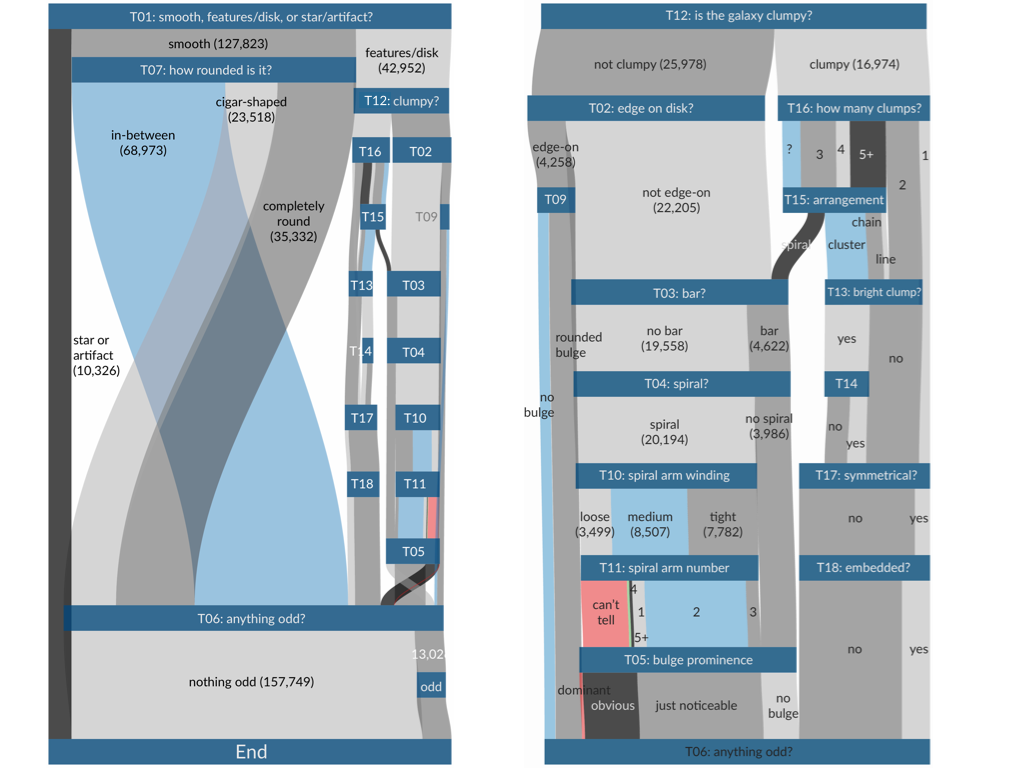
\includegraphics[width=0.90\textwidth]{figures/sankey_both.png}
\caption{Demographics of the morphologies for all galaxies in GZH (including
both \hst{} and SDSS imaging). Each node in each diagram (dark blue horizontal
bars of uniform height) represents a task in the tree. The left diagram shows
the full decision tree; the right diagram zooms in on the features/clumpy
tasks, which are otherwise difficult to see. The paths between tasks represent
each possible answer to the task; these flow from top to bottom between their
origin question and the subsequent task in the tree. Labels are assigned to
each galaxy based on the plurality answer for each task. A galaxy is assigned
only one label at each node. Widths of the paths are proportional to the number
of galaxies assigned to that path; the widths of the nodes are proportional to
the number of galaxies for which the question was reliably answered.}
\label{fig:sankey}
\end{figure*}

Given these caveats, the overall distribution of galaxy types is significantly
different than the low-redshift sample classified in SDSS imaging from GZ1 and
GZ2. \citet{lin11} found that elliptical galaxies exceeded spiral galaxies by a
factor of $\sim2:1$ in the main spectroscopic sample if using a plurality vote
criterion (although \citealt{bam09} show that this strongly depends on the
selection method; spirals are the dominant population in a volume-limited
sample at $z<0.088$, for example). The weighted votes for GZH have smooth
galaxies outnumbering disks and clumpy galaxies by a factor of $\sim3:1$,
however. The fraction of objects identified as stars or artifact is also much
higher in the Hubble imaging; by plurality votes, these encompass only
$\sim0.1\%$ of images in SDSS \citep{wil13}, but 6\% of images in GZH. 

Within the sample of galaxies identified as ``not smooth'', it is clear that
the addition of the clumpy branch is necessary to describe a large fraction of
the sample; disk-dominated galaxies outnumber clumpy morphologies by less than
a factor of 2. Disk galaxies are primarily unbarred \citet{mel14} and
possessing two visible spiral arms over a flat distribution of pitch angles and
bulge prominence. Clumpy galaxies are identified across the full range of clump
multiplicities, with the exception of 1-clump galaxies (which would be
difficult to differentiate from compact spheroids). Roughly half of the
galaxies have at least 1~clump identified as the brightest; the clumps are most
commonly asymmetrically arranged in clusters and are not often seen embedded in
larger structures. 

\subsection{Comparing GZH morphologies to other catalogs}\label{ssec:comparisons}

All of the Legacy surveys included in the GZH imaging have had morphological
catalogs previously published; these catalogs have significant differences in
the number of galaxies, size and magnitude limits, classification scheme, and
the methods used for measuring morphology. These catalogs have been
cross-matched to GZH to compare the results; this is not presented as an
endorsement of any particular method, but as an exploration of the strengths
and weaknesses of the GZ crowdsourced catalogs as compared to products made
with machine learning, automatic fits, and expert visual classification. 

The types and accuracy of morphological classification strongly depend on the
sample and methods being used. In an attempt to make a consistent comparison
between different techniques, galaxies are broadly grouped into three
categories: bulge-dominated/elliptical/smooth, disk-dominated/spiral, and
irregular/clumpy. These categories are compared to two parameters in GZH:
\fbest, which is designed to identify smooth (elliptical) galaxies, and \fodd,
which is designed to identify deviations from well-formed spirals or S0s and
which constitutes a ``catch-all'' for the variety of asymmetric morphologies
that can constitute an irregular galaxy. 

Morphologies for GEMS galaxies were measured by \citet{hau07}, who used
single-component \sersic{} fits to the F850LP imaging. This analysis used
parameters from the \galfit{} code, which \citet{hau07} evaluated as more
reliable than \gimtwod{} for GEMS due to the ability to fit multiple galaxies
in crowded fields. A 1\arcsec~positional match for the GEMS galaxies in Table~9
in \citet{hau07} to the GZH sample gives 8,846~galaxies in both \citet{hau07}
and GZH. The main morphological parameter in the automated catalog is the
\sersic{} index $n$ defining the radial surface brightness profile.
``Elliptical'' galaxies are selected by $n>2.5$ and ``spirals''  by $n>2.5$.
There is no automatic measurement of irregular or clumpy structure in this
catalog. 

AEGIS galaxies were morphologically classified using non-parametric
measurements by \citet{lot08}. This method used a combination of the Gini
coefficient ($G$), which measures the relative inequality in pixel brightness,
and $M_{20}$, the second-order moment of the brightest 20\% of the light
\citep{lot04}. A linear combination of $G$ and $M_{20}$ delineates three broad
categories of galaxy morphology: E/S0/Sa (``elliptical''), Sb/Sc/Ir
(``spiral''), and mergers (``irregular''). A 1\arcsec{} positional match on
AEGIS and GZH yields 4,031 galaxies with reliably-measured morphologies and
$S/N>3$ in both $V$- and $I$-bands. 

Galaxies in both of the GOODS fields down to a limit of $z_{AB}=22.5$ were
visually classified by a single expert (R.S.~Ellis), inspecting both $z$-band
and composite $Viz$ color images \citep{bun05}. These morphologies are assigned
a numerical value based on categories in \citet{bri98a}; the corresponding
morphologies used are ``elliptical'' (classes 0,1,2), ``spirals'' (classes
3,4,5), and ``irregular'' (classes 6,7,8). A 0.5\arcsec{} matched radius yields
2,435 galaxies (1300 in GOODS-N, 1135 in GOODS-S) in both \citet{bun05} and
GZH.  

COSMOS galaxies have multiple published datasets automatically classifying
morphology, all using a variation of non-parametric measurements. \citet{cas07}
used a combination of concentration ($C$), asymmetry ($A$), $G$, and $M_{20}$
\citep{cas05} to classify all galaxies with $m_\mathrm{I,petro}<25$, and used
an empirical division based on several hundred training images to assign
galaxies to discrete morphological categories. A similar method is employed by
\citet{tas11}, using the same non-parametric indices but with a different
method of calculating the Petrosian radius and total light profile. They employ
a nearest-neighbors method is used to assign morphological categories for the
entire sample based on a small training set. \citet[][ZEST]{sca07} used $C$,
$A$, $G$, $M_{20}$, the galaxy ellipticity ($\epsilon$), and \sersic{} index
($n$) to quantify the galaxy shapes; a principal component analysis is used to
assign galaxies to discrete morphological categories. The categories in all
three methods are split into ellipticals, spirals, and peculiar/irregulars. A
0.5\arcsec{} radius search on GZH matches to 76,241 galaxies in \citet{cas07},
76,608 in \citet{tas11}, and 77,425 in \citet{sca07}.

\begin{figure*}
\center
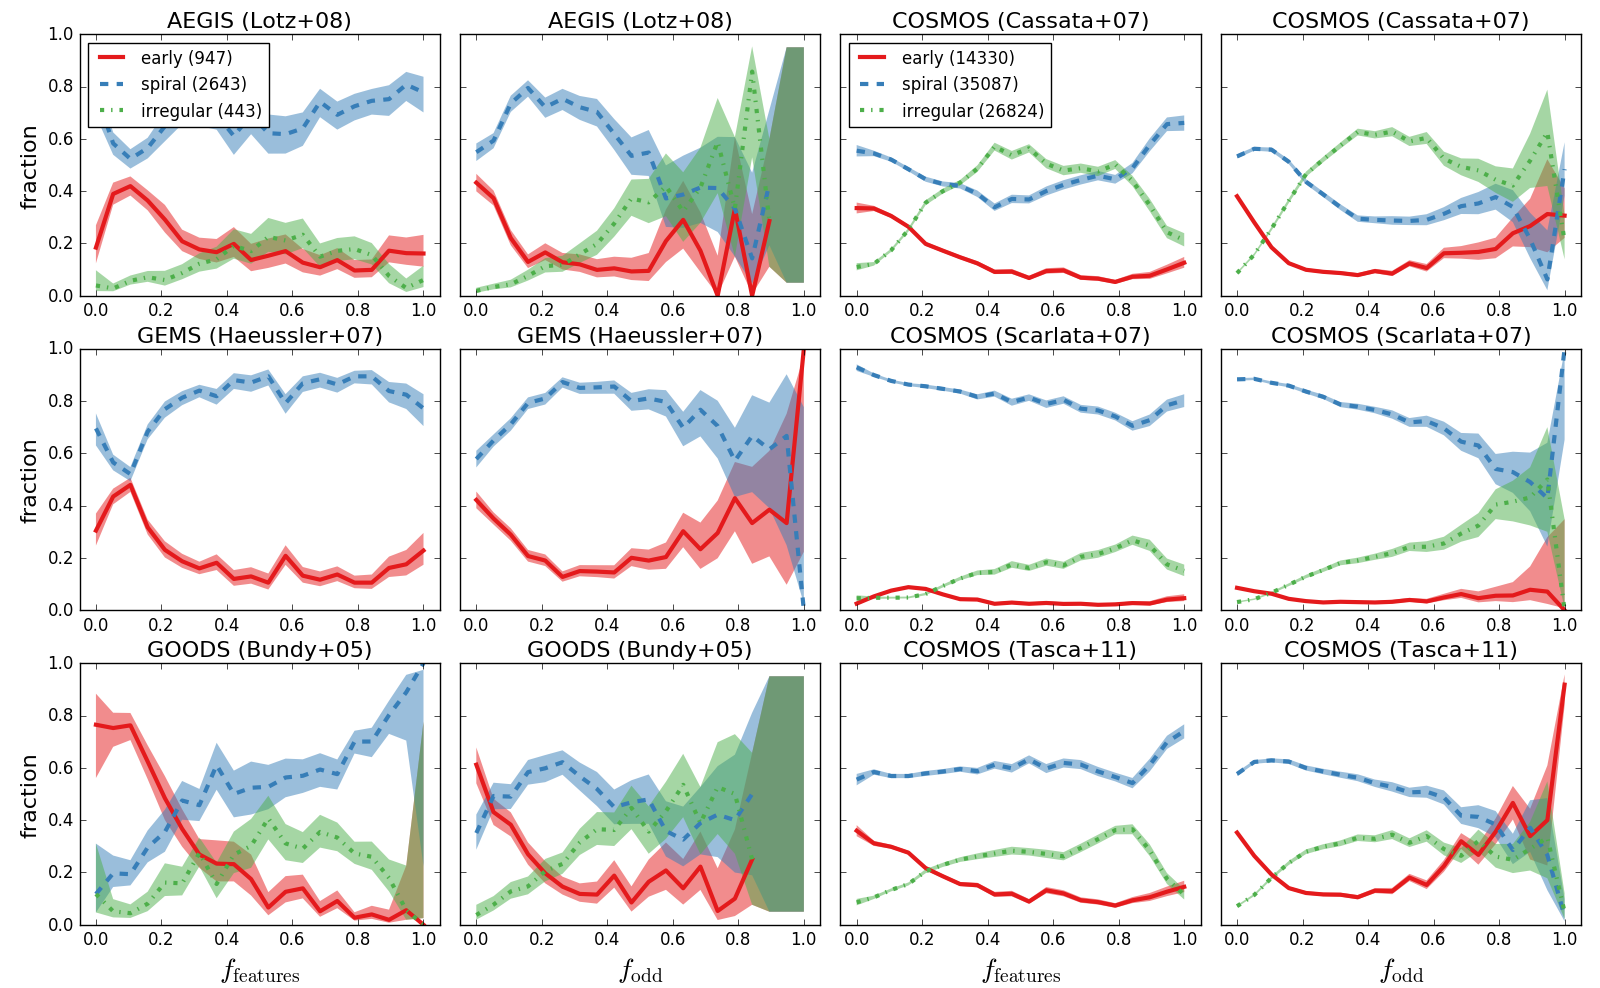
\includegraphics[width=1.0\textwidth]{figures/comparisons.png}
\caption{Distributions of morphological parameters for galaxies matched in GZH
and other published catalogs, split by survey (AEGIS, COSMOS, GEMS, and GOODS).
The first and third columns show the fraction of overall galaxies in the
matched samples, split by their published morphologies as a function of the GZH
\fbest. The corresponding second and fourth columns show data for the same
galaxies as a function of \fodd. Confidence intervals for each binned fraction
in the bin are calculated for a binomial population \citep{cam11}.}
\label{fig:comparisons}
\end{figure*}

Figure~\ref{fig:comparisons} shows the proportion of galaxies as split by their
automated/expert visual morphologies for each of the six catalogs matched to
GZH. The relation between GZH and the automated/expert morphologies is shown to
vary significantly for different surveys --- this could be due to intrinsic
differences in the galaxies, in the techniques used to measure morphology, or
both. The distribution of \fbest{} for AEGIS galaxies is essentially flat for
spirals, showing almost no difference in proportion at the highest and lowest
ends. Early-type galaxies are at their highest proportion at \fbest$\sim0$, but
constitute at most only 40\% of galaxies. In contrast, GOODS galaxies at low
\fbest{} are dominated by early-types, although spiral and irregular galaxies
have comparable sizes as low as \fbest$\sim0.2$. In GEMS galaxies, the impact
of irregular or peculiar galaxies is not measured; splitting on $n=2.5$ gives
an essentially flat proportion of ellipticals to spirals at \fbest$>0.3$.
Visual inspection of images of galaxies where both \fbest{} and $n$ are high
show that the majority are obvious spirals but with prominent bulges,
indicating that the single-component \sersic{} fit is likely choosing too small
of an effective radius and missing the extended disk structure for a large
population of galaxies. 

Even within the same sample of galaxies in COSMOS, different techniques of
measuring morphology show significant differences. Both \citet{cas07} and
\citet{tas11} have higher proportions of early-type galaxies at \fbest$\sim0$,
but constitute less than half the sample in both cases. The majority of all
galaxies in \citet{sca07}, in contrast, are spirals; oddly, the \emph{highest}
proportions of spirals are found at the lowest values of \fbest. The decrease
in spiral galaxies at higher \fbest{} is almost entirely balanced by an
increase in irregulars. Early-types have a small bump near \fbest$\sim0.15$,
but never constitute more than 10\% of the sample. 

The second set of plots in Figure~\ref{fig:comparisons} indicates that \fodd{}
is largely an effective method for separating irregular and/or peculiar
galaxies from spirals. Despite the somewhat vague wording of the {\it
``anything odd?''} question in GZH, the AEGIS, COSMOS, and GOODS all show a
marked increase in the irregular fraction increasing with \fodd. Any threshold
value for distinguishing between the two, however, depends strongly on
survey/redshift~range. 

As the data shown in Figure~\ref{fig:comparisons} cover a wide range of
redshifts and sizes, a volume-limited sample of galaxies (or at least binning
by redshift) is likely a much more appropriate comparison. While detailed
analysis is left to a further paper, we note that there is no strong change in
the proportion of galaxies when binning by redshift intervals of $\Delta z=0.2$
out to $z=1.0$. 

Finally, there are 7,681~galaxies in the GOODS-S field with morphological
classifications in both GZH and the Galaxy~Zoo:~CANDELS project (Simmons
et~al., submitted). Since both the sensitivity and filters for the two sets of
images differ (and there is no debiased correction applied to GZC), there is no
prior reason to expect a perfect correlation between the separate vote
fractions for the projects. Briefly, we note that the \ffeatures{} value for
GZH is on average higher than GZC; the effect is strongest at
$f_\mathrm{features,GZC}<0.3$, for which roughly half the galaxies have
$f_\mathrm{features,GZH}>0.5$. However, the correlation between vote fractions
is single-valued (although not linear, with a Pearson correlation coefficient
of $r=0.6$), and should be possible to calibrate using a similar approach to
that described in Section~\ref{sec:debiasing}; the correlation between other
tasks, such as edge-on galaxies is significantly stronger ($r=0.9$). So while
the raw vote fractions are not directly comparable, the initial analysis
indicates that the broad morphologies are at least consistent.

\section{Summary}\label{sec:summary}

%Now people go and do science with these awesome GZH classifications. 

This paper presents the catalog release for the Galaxy Zoo: Hubble project,
which uses crowdsourced visual classifications to measure galaxy morphologies.
The first two phases of Galaxy Zoo \citep{lin11,wil13} used images of
low-redshift galaxies from SDSS; this is the first result of the project with
space-based images of high-redshift targets (in addition to the Galaxy Zoo:
CANDELS collaboration; Simmons et al., submitted). The final sample includes
classifications for 181,101~images generated from 150,771~unique galaxies.
Galaxies were selected from a brightness-limited sample from multiple Legacy
surveys using the Advanced Camera for Surveys on the Hubble Space Telescope,
including AEGIS, GEMS, GOODS-N, GOODS-S, and COSMOS. The catalog also includes
classifications for 51,861 Sloan Digital Sky Survey images in Stripe~82 at
relatively low redshift; these serve both as a low-redshift anchor for
cosmological studies and a potential comparison for the different epochs of
classification between GZH and Galaxy Zoo 2 \citep{wil13}. 

The data for the GZH catalogs has been extensively tested and reduced. The
dominant effect is a known bias against identifying disky and asymmetric
sub-structures at either low resolution or surface brightness. This can be the
result either of genuinely small or dim galaxies, or a perceived effect from
observing galaxies at further distances (higher redshift). To calibrate this
\emph{without} potentially overcorrecting for the genuine morphological
evolution of galaxies over cosmic time, the GZH project uses SDSS images of
low-redshift galaxies, processes them to appear as if they were at higher
redshift, and classifies them through the GZH interface in an identical
fashion. The resulting change in \ffeatures{} as a function of $z$ and $\mu$ is
applied as a multiplicative correction to the top-level vote fractions for
$\sim50\%$ of the GZH galaxies. 

Galaxies in GZH show significant changes in the disk/elliptical fraction as a
function of redshift, along with an increasing number of galaxies dominated by
smaller clumps and presumed to be in the process of building up their baryonic
mass through a combination of hierarchical merging and in-situ star formation.
While the majority of scientific interpretation is left to future work, this
paper confirms the decrease in observed bar fraction with increasing redshift
\citep{mel14} and identifies a new way for selecting clumpy galaxies as a
function of clump multiplicity.

The full data tables for the catalogs can be accessed in machine-readable form
from both the journal and at \url{http://data.galaxyzoo.org}. All the code and
data tables used to generate this manuscript can be found at
\url{https://github.com/willettk/gzhubble}.
 
\acknowledgments

We thank Meg Schwamb and the ASIAA for hosting the ``Citizen Science in
Astronomy'' workshop, 3-7 Mar 2014 in Taipei, Taiwan, at which some of this
analysis was done. We thank Jennifer Lotz for sharing her $G$-$M_{20}$
measurements for the AEGIS sample. We thank Coleman Krawczyk for his assistance
in producing Figure~\ref{fig:decisiontree}.

This project made heavy use of the Astropy packages in Python \citep{ast13},
the \texttt{seaborn} plotting package \citep{was15}, astroML \citep{van12}, and
TOPCAT \citep{tay05,tay11}. Modified code from Nick~Wherry and David~Schlegel
was used to create the JPG images. Figure~\ref{fig:sankey} was generated with
\url{http://sankeymatic.com/}.

KS gratefully acknowledges support from Swiss National Science Foundation Grant
PP00P2\_138979/1.

This work is based on (GO-10134, GO-09822, GO-09425.01, GO-09583.01, GO-9500)
program observations with the NASA/ESA Hubble Space Telescope, obtained at the
Space Telescope Science Institute, which is operated by the Association of
Universities for Research in Astronomy, Inc., under NASA contract NAS 5-26555. 

Funding for the SDSS and SDSS-II has been provided by the Alfred P. Sloan
Foundation, the Participating Institutions, the National Science Foundation,
the U.S. Department of Energy, the National Aeronautics and Space
Administration, the Japanese Monbukagakusho, the Max Planck Society, and the
Higher Education Funding Council for England. The SDSS website is
\url{http://www.sdss.org/}. 

The SDSS is managed by the Astrophysical Research Consortium for the
Participating Institutions. The Participating Institutions are the American
Museum of Natural History, Astrophysical Institute Potsdam, University of
Basel, University of Cambridge, Case Western Reserve University, University of
Chicago, Drexel University, Fermilab, the Institute for Advanced Study, the
Japan Participation Group, Johns Hopkins University, the Joint Institute for
Nuclear Astrophysics, the Kavli Institute for Particle Astrophysics and
Cosmology, the Korean Scientist Group, the Chinese Academy of Sciences
(LAMOST), Los Alamos National Laboratory, the Max-Planck-Institute for
Astronomy (MPIA), the Max-Planck-Institute for Astrophysics (MPA), New Mexico
State University, Ohio State University, University of Pittsburgh, University
of Portsmouth, Princeton University, the United States Naval Observatory and
the University of Washington. 

\bibliography{gz_hubble_data}

\newpage
\clearpage

\appendix

\section{GOODS Shallow Depth data}


\begin{table}
\caption{Correctable fractions for the top-level task in GZH in the GOODS shallow-depth (2-epoch) images. \label{tbl:goods_shallow_categories}}
\begin{tabular}{lrrrrrrrr}
\hline\hline
                                   & GOODS-N & GOODS-S & Total \\
\hline
Correctable                        & 748     & 514     & 1,262 \\
Lower limit                        & 526     & 1,143   & 1,669 \\
No Correction Needed ($z \le 0.3$) & 267     & 267     & 534   \\ 
NEI                                & 851     & 2,670   & 3,521 \\
No Redshift Information            & 159     & 319     & 478   \\
Total                              & 2,551   & 4,913   & 7,464 \\
\hline\hline
\end{tabular}
\end{table}

GZH used both 5-epoch and 2-epoch sets of data to construct the GOODS set of
images. The 11,157 full depth 5-epoch images are used in the main catalog; the
classifications for the 7,464 shallow depth 2-epoch images are provided as a
supplementary table. This section analyzes the effect of image depth on the
ability of the GZ classifiers to identify features or disk structure in the images. 

\subsection{Comparing shallow and full depth morphologies}

Of the 11,157 galaxies in the GOODS-N and GOODS-S full depth sample, 4,461 of
these are in the shallow-depth sample. Figure~\ref{fig:shallow_vs_full} shows a
strong correlation between \ffeatures{} for both sets of images. The mean
change in \ffeatures{} from the shallow to full depth images
$f_\mathrm{features,full} - f_{features,shallow} \equiv \Delta f = 0.00$, with
a standard deviation of $\sigma = 0.17$. While there is some variance in
$\Delta f$ in the whole sample, the change is usually small and not often
significant enough to change a morphological classification. Defining a clean
sample of disk galaxies as those with \fbest$>0.8$, elliptical galaxies as
those with $f_\mathrm{smooth,best}<0.2$, and intermediate as those in between,
75\% of the sample would not change morphology. Of the remaining 25\% that
would change morphology, only 0.3\% (representing 10 galaxies total)
drastically change morphology from smooth to featured or vice versa, while the
rest would transition to or from the ``intermediate'' morphology. Details can
be seen in Table~\ref{tbl:shallow_to_full_stats} and examples of images
representing the 9 possible changes (or lack of) in morphology are shown in
Figures~\ref{fig:shallow_smooth},\ref{fig:shallow_intermediate}, and
\ref{fig:shallow_featured}.

\begin{figure*}
\begin{center}
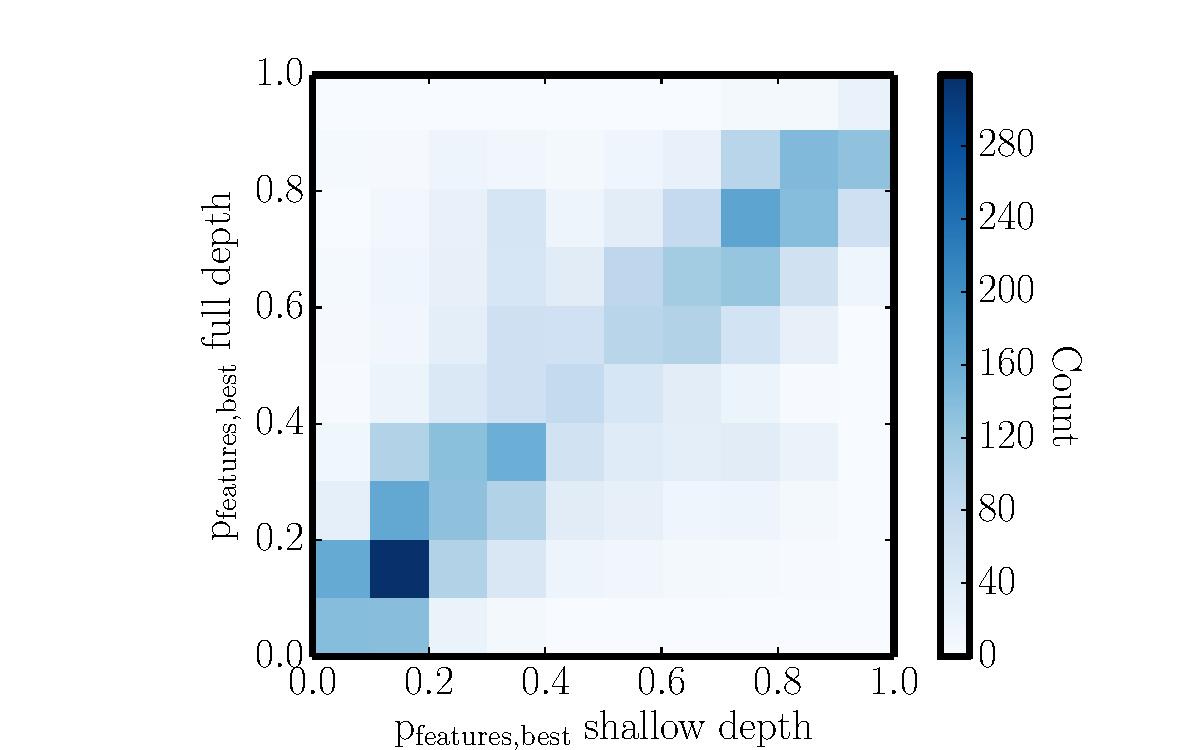
\includegraphics[width=0.50\textwidth]{figures/full_shallow_p_plot.pdf}
\caption{Distribution of \ffeatures{} for the 4,461 GOODS galaxies with both
shallow (2-epoch) and full-depth (5-epoch) images morphologically classified in
GZH. For most galaxies, the value of \ffeatures{} is consistent ($\Delta
f_\mathrm{features}<0.2$) between depths. Examples of galaxies with sharp
changes in \ffeatures, as well as those with little to no change are shown in
Figures~\ref{fig:shallow_smooth}-\ref{fig:shallow_featured}.}
\label{fig:shallow_vs_full}
\end{center}
\end{figure*}

\begin{table}
\caption{Properties of galaxies whose morphologies changed or stayed the same
in the shallow vs full images. Featured here is defined as \fbest$>0.8$,
intermediate = $0.2<$\fbest$<0.8$, smooth = $f_\mathrm{smooth,best}<0.2$.
\label{tbl:shallow_to_full_stats}}
\begin{tabular}{lrrrrrrrr}
\hline\hline
shallow to full morphology    & N       & \%       & $<\Delta f>$ & $<z>$ \\
\hline
smooth to smooth              & 758     & 17.0     & -0.00        &  0.69\\
smooth to intermediate        & 367     & 8.2      & 0.18         &  0.69\\
smooth to featured            & 7       & 0.2      & 0.76         &  0.57\\ 
intermediate to smooth        & 214     & 4.8      & -0.18        &  0.65\\
intermediate to intermediate  & 2,303   & 51.6     & 0.01         &  0.78 \\
intermediate to featured      & 168     & 3.8      & 0.19         &  0.83\\
featured to smooth            & 3       & 0.1      & -0.74        &  0.71\\
featured to intermediate      & 337     & 7.6      & -0.18        &  0.68\\
featured to featured          & 301     & 6.8      & -0.05        &  0.71\\

Total                         & 4,461   & 100      &              & \\
\hline\hline
\end{tabular}
\end{table}



\begin{figure*}
\centering

\subfigure{[a]\label{fig:smooth_to_smooth}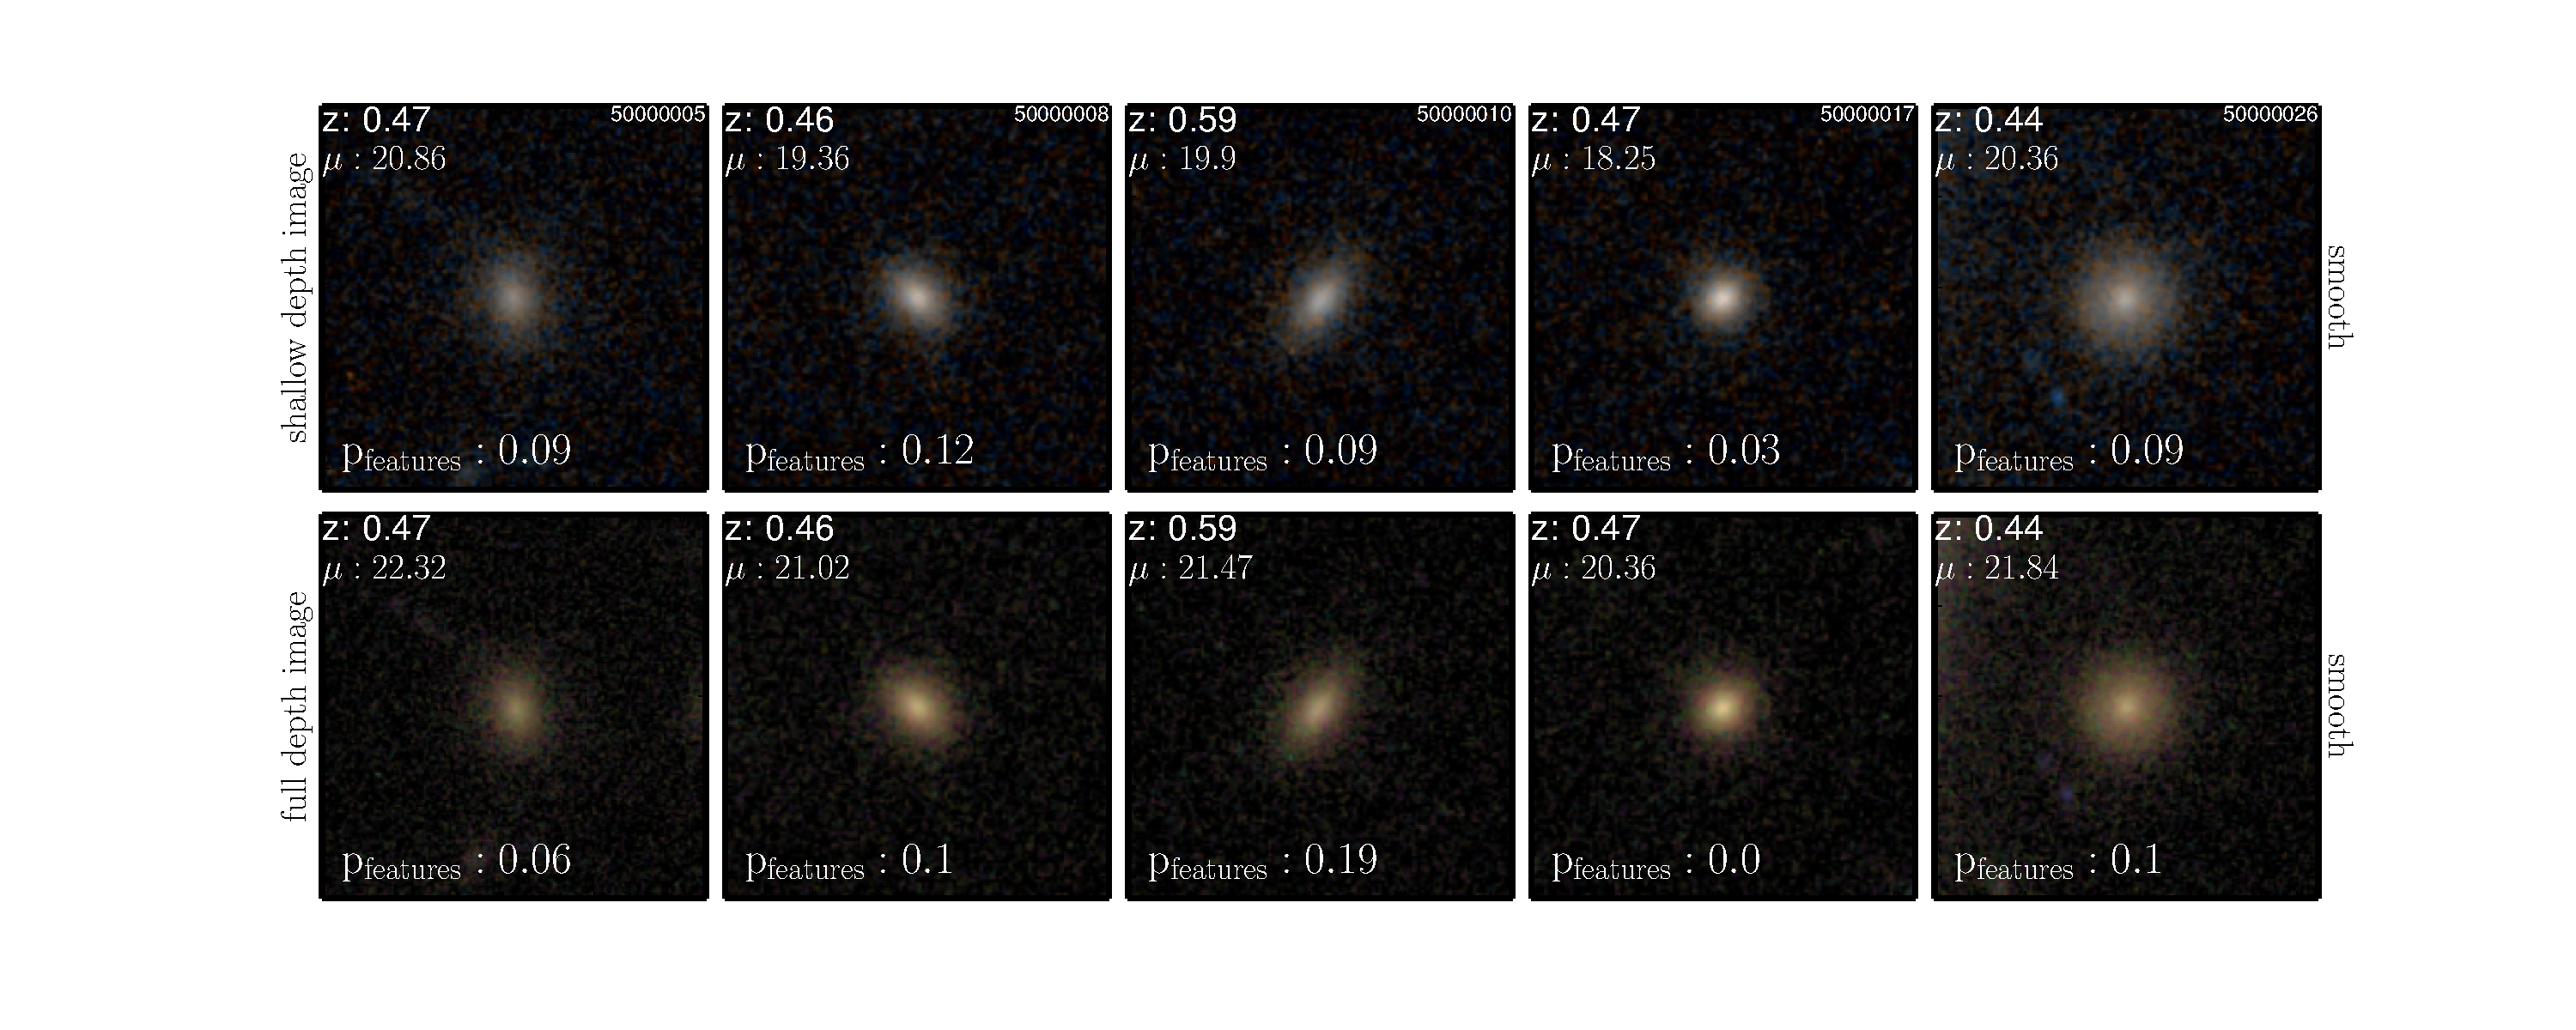
\includegraphics[width=\textwidth]{figures/smooth_to_smooth.pdf}}

\subfigure{[b]\label{fig:smooth_to_int}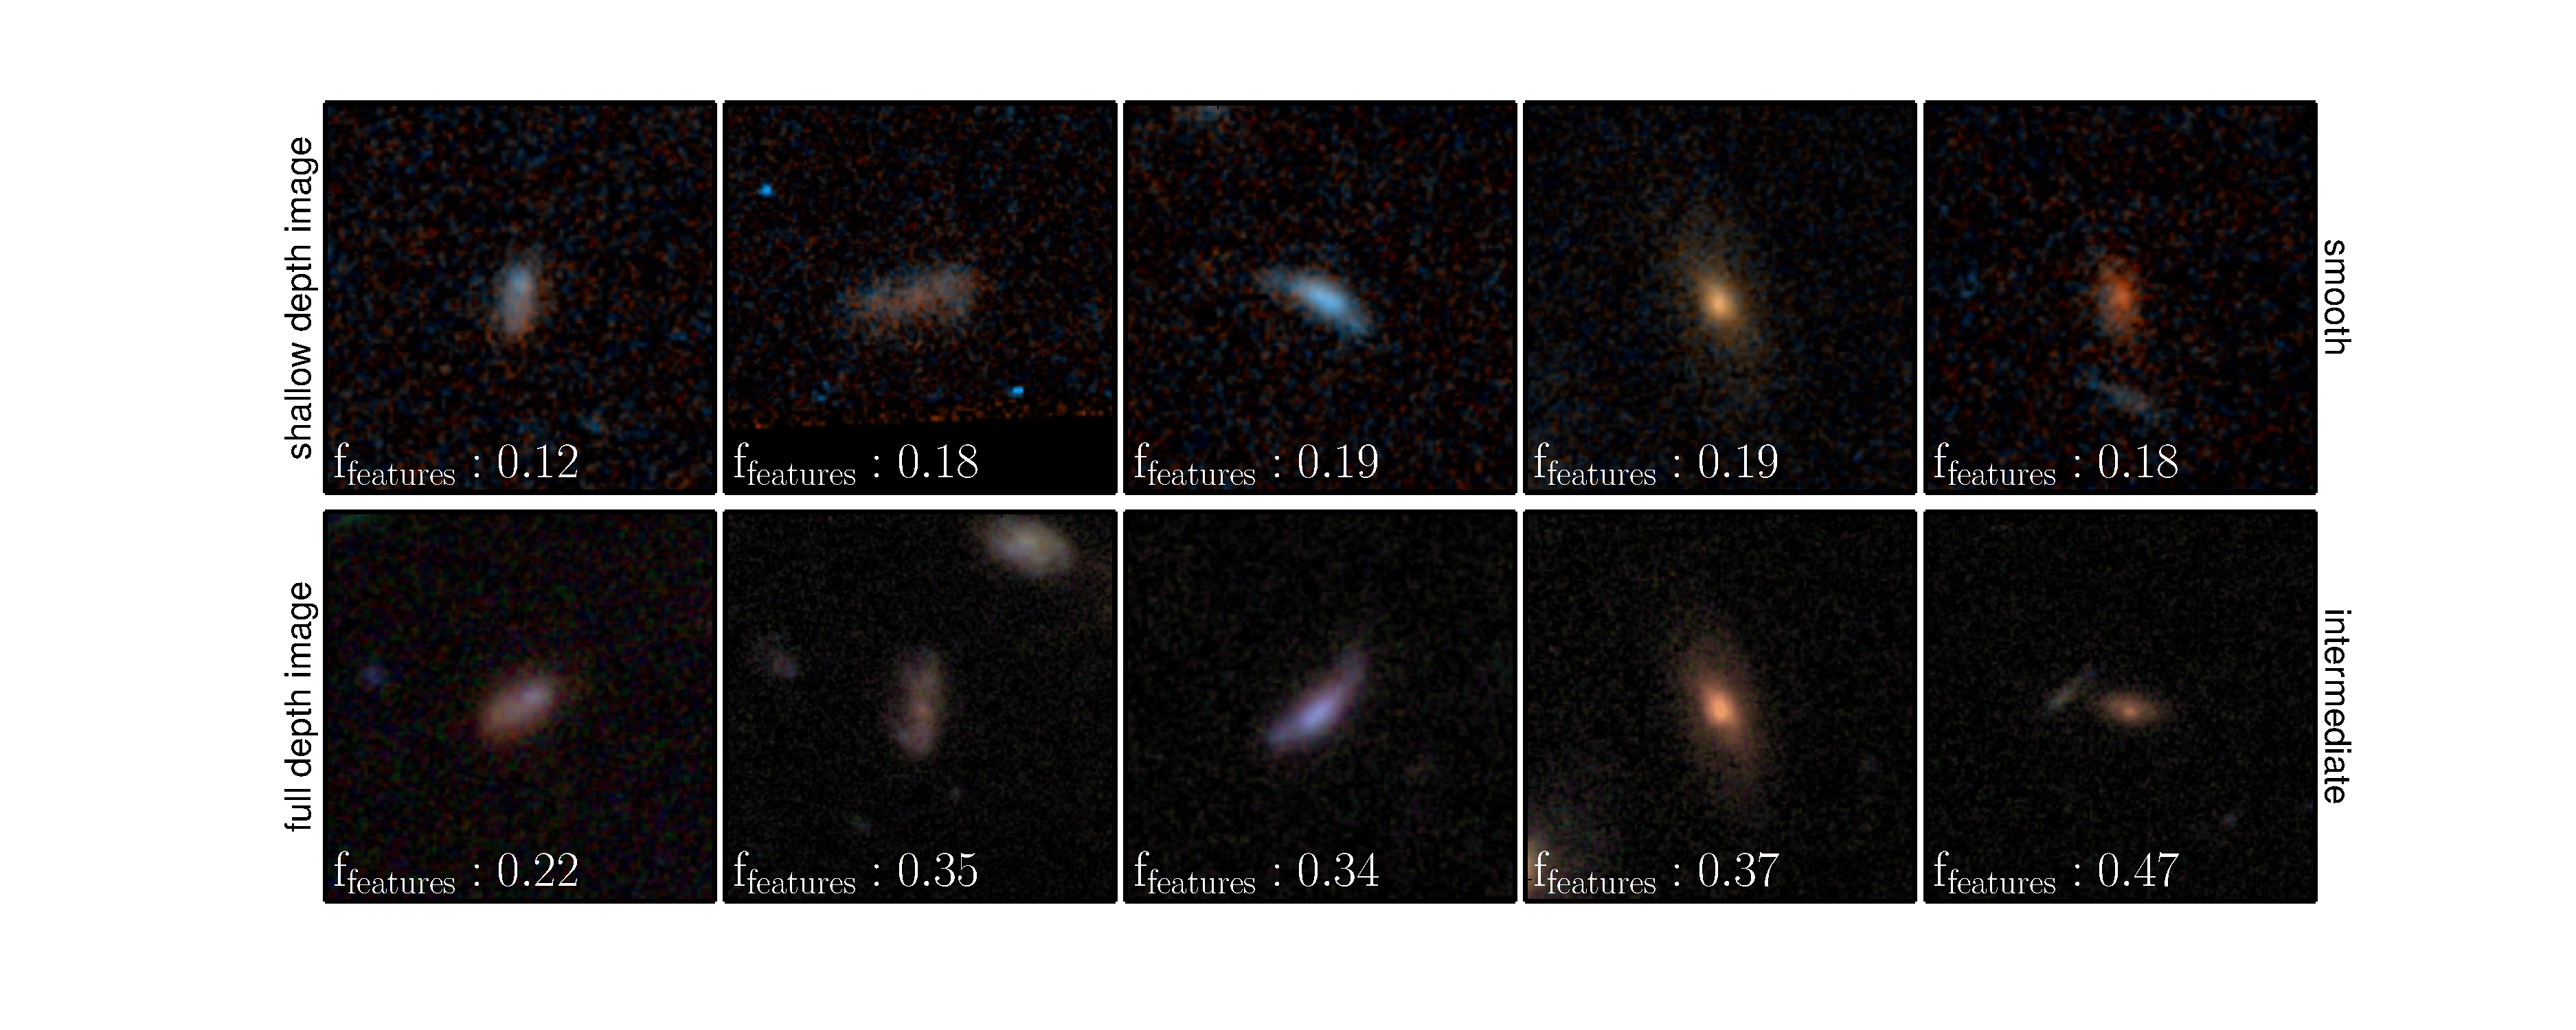
\includegraphics[width=\textwidth]{figures/smooth_to_intermediate.pdf}}

\subfigure{[c]\label{fig:smooth_to_featured}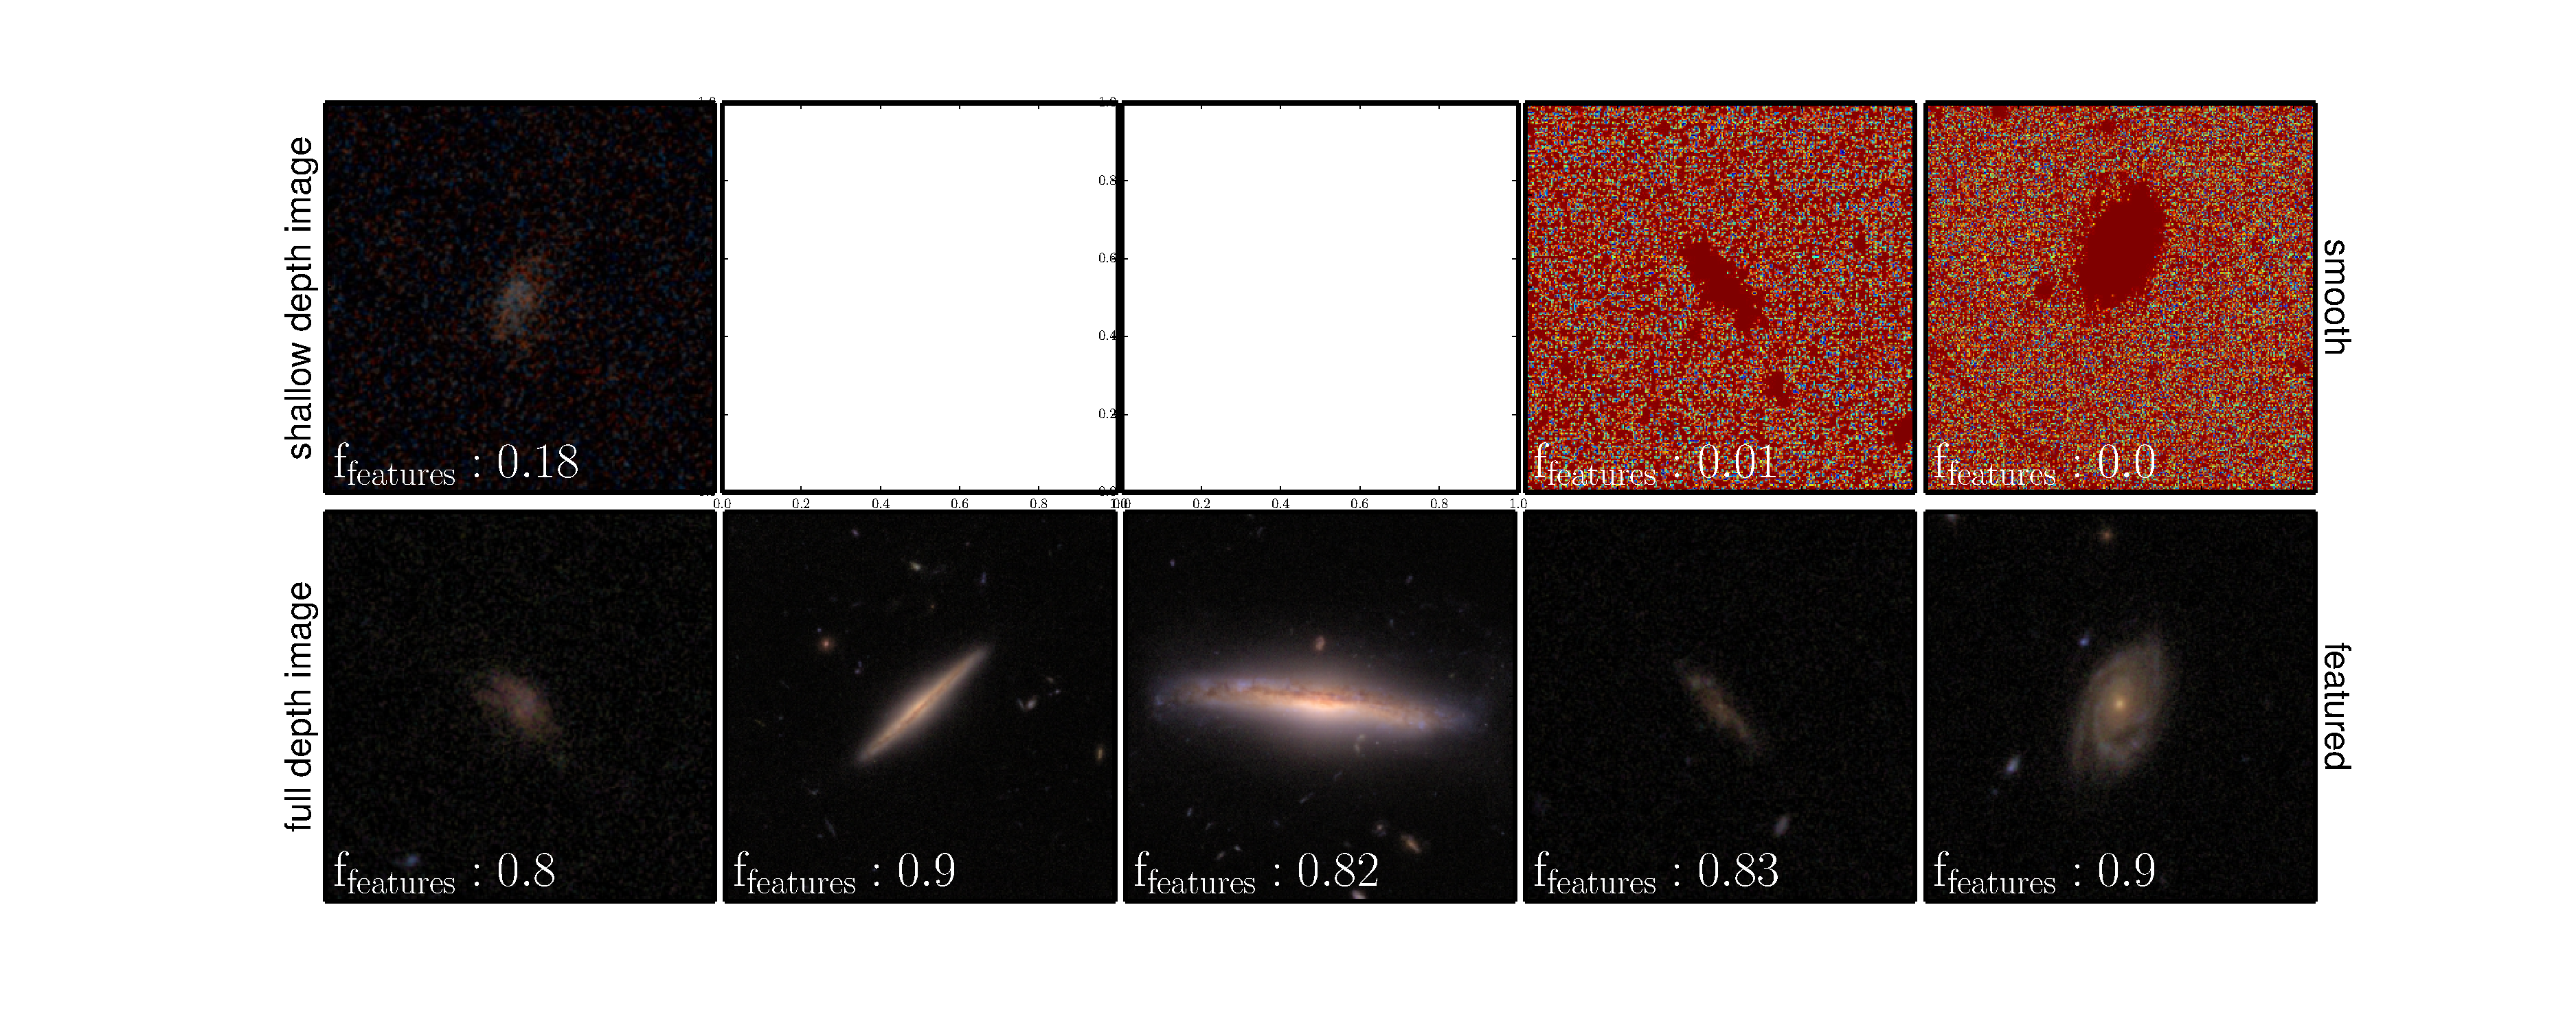
\includegraphics[width=\textwidth]{figures/smooth_to_featured.pdf}}

\caption{Galaxies whose shallow images were classified as smooth and full depth images were classified as smooth, intermediate, or featured.}
\label{fig:shallow_smooth}
\end{figure*}

\begin{figure*}
\centering

\subfigure{[b]\label{fig:int_to_smooth}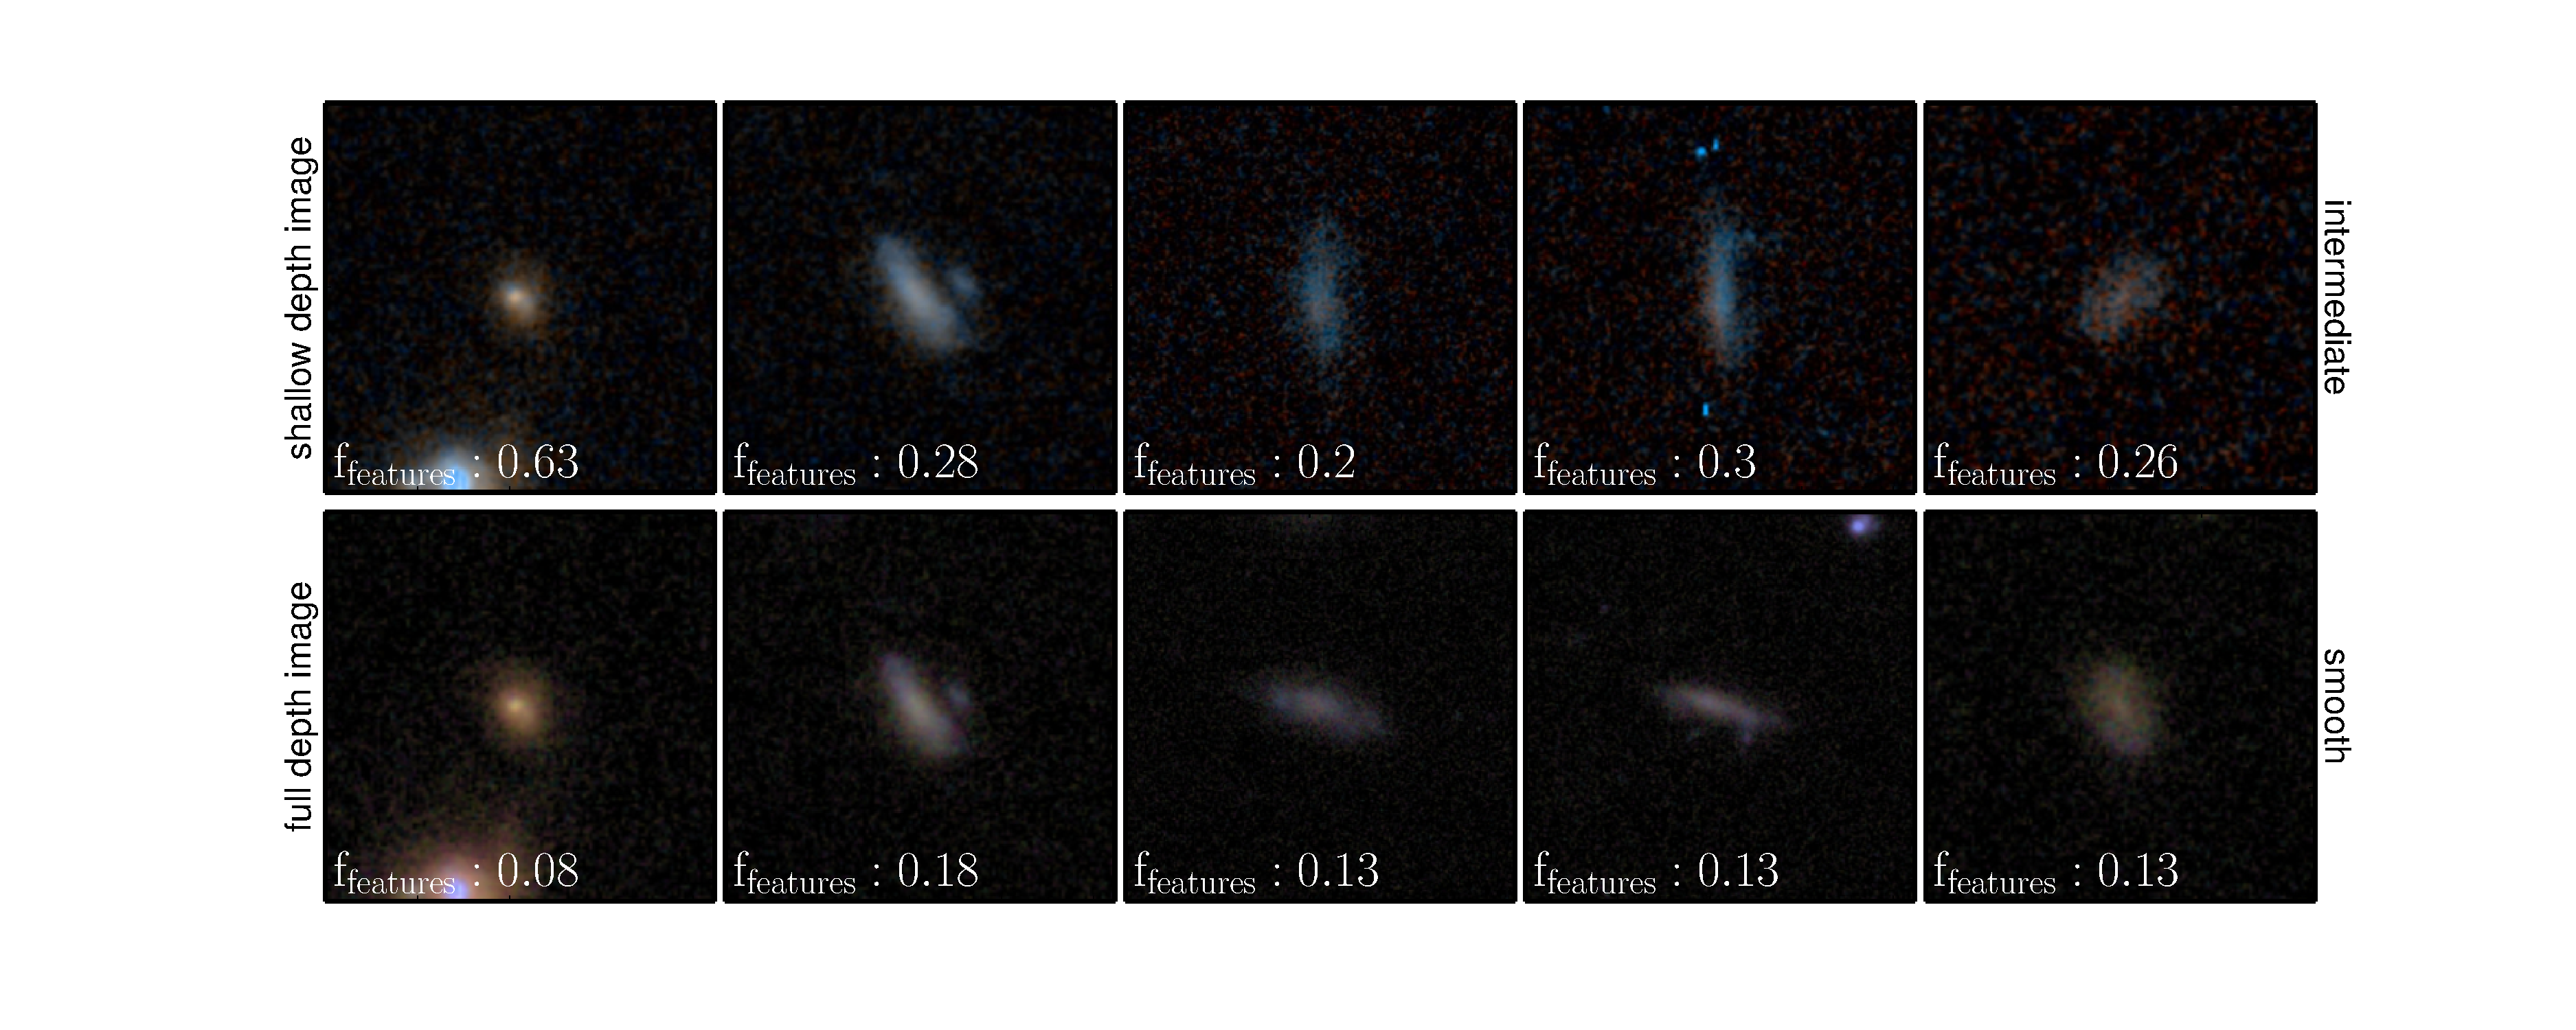
\includegraphics[width=\textwidth]{figures/intermediate_to_smooth.pdf}}

\subfigure{[b]\label{fig:int_to_int}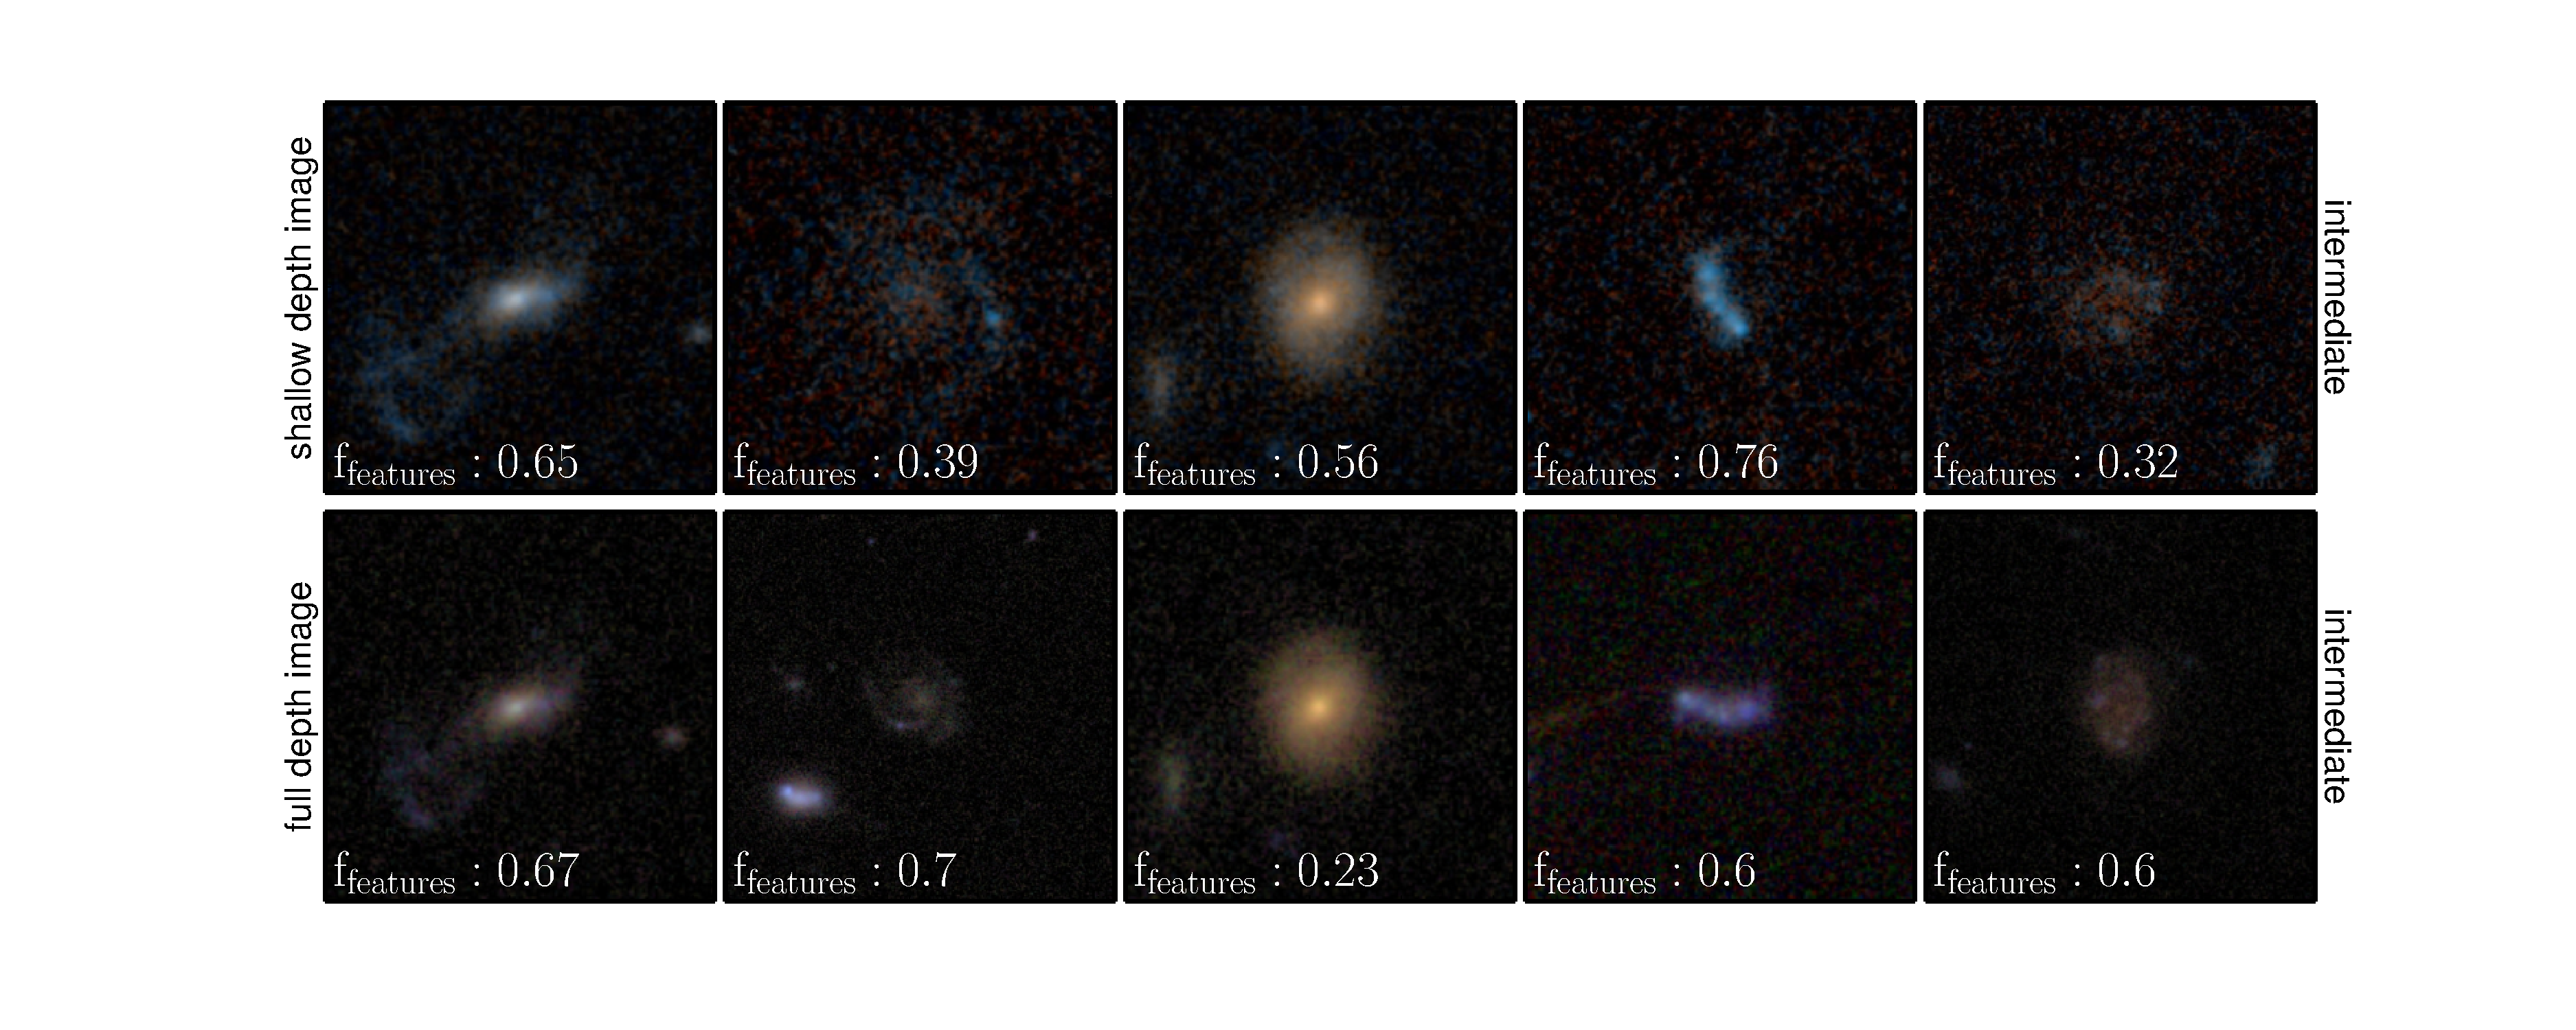
\includegraphics[width=\textwidth]{figures/intermediate_to_intermediate.pdf}}

\subfigure{[b]\label{fig:int_to_featured}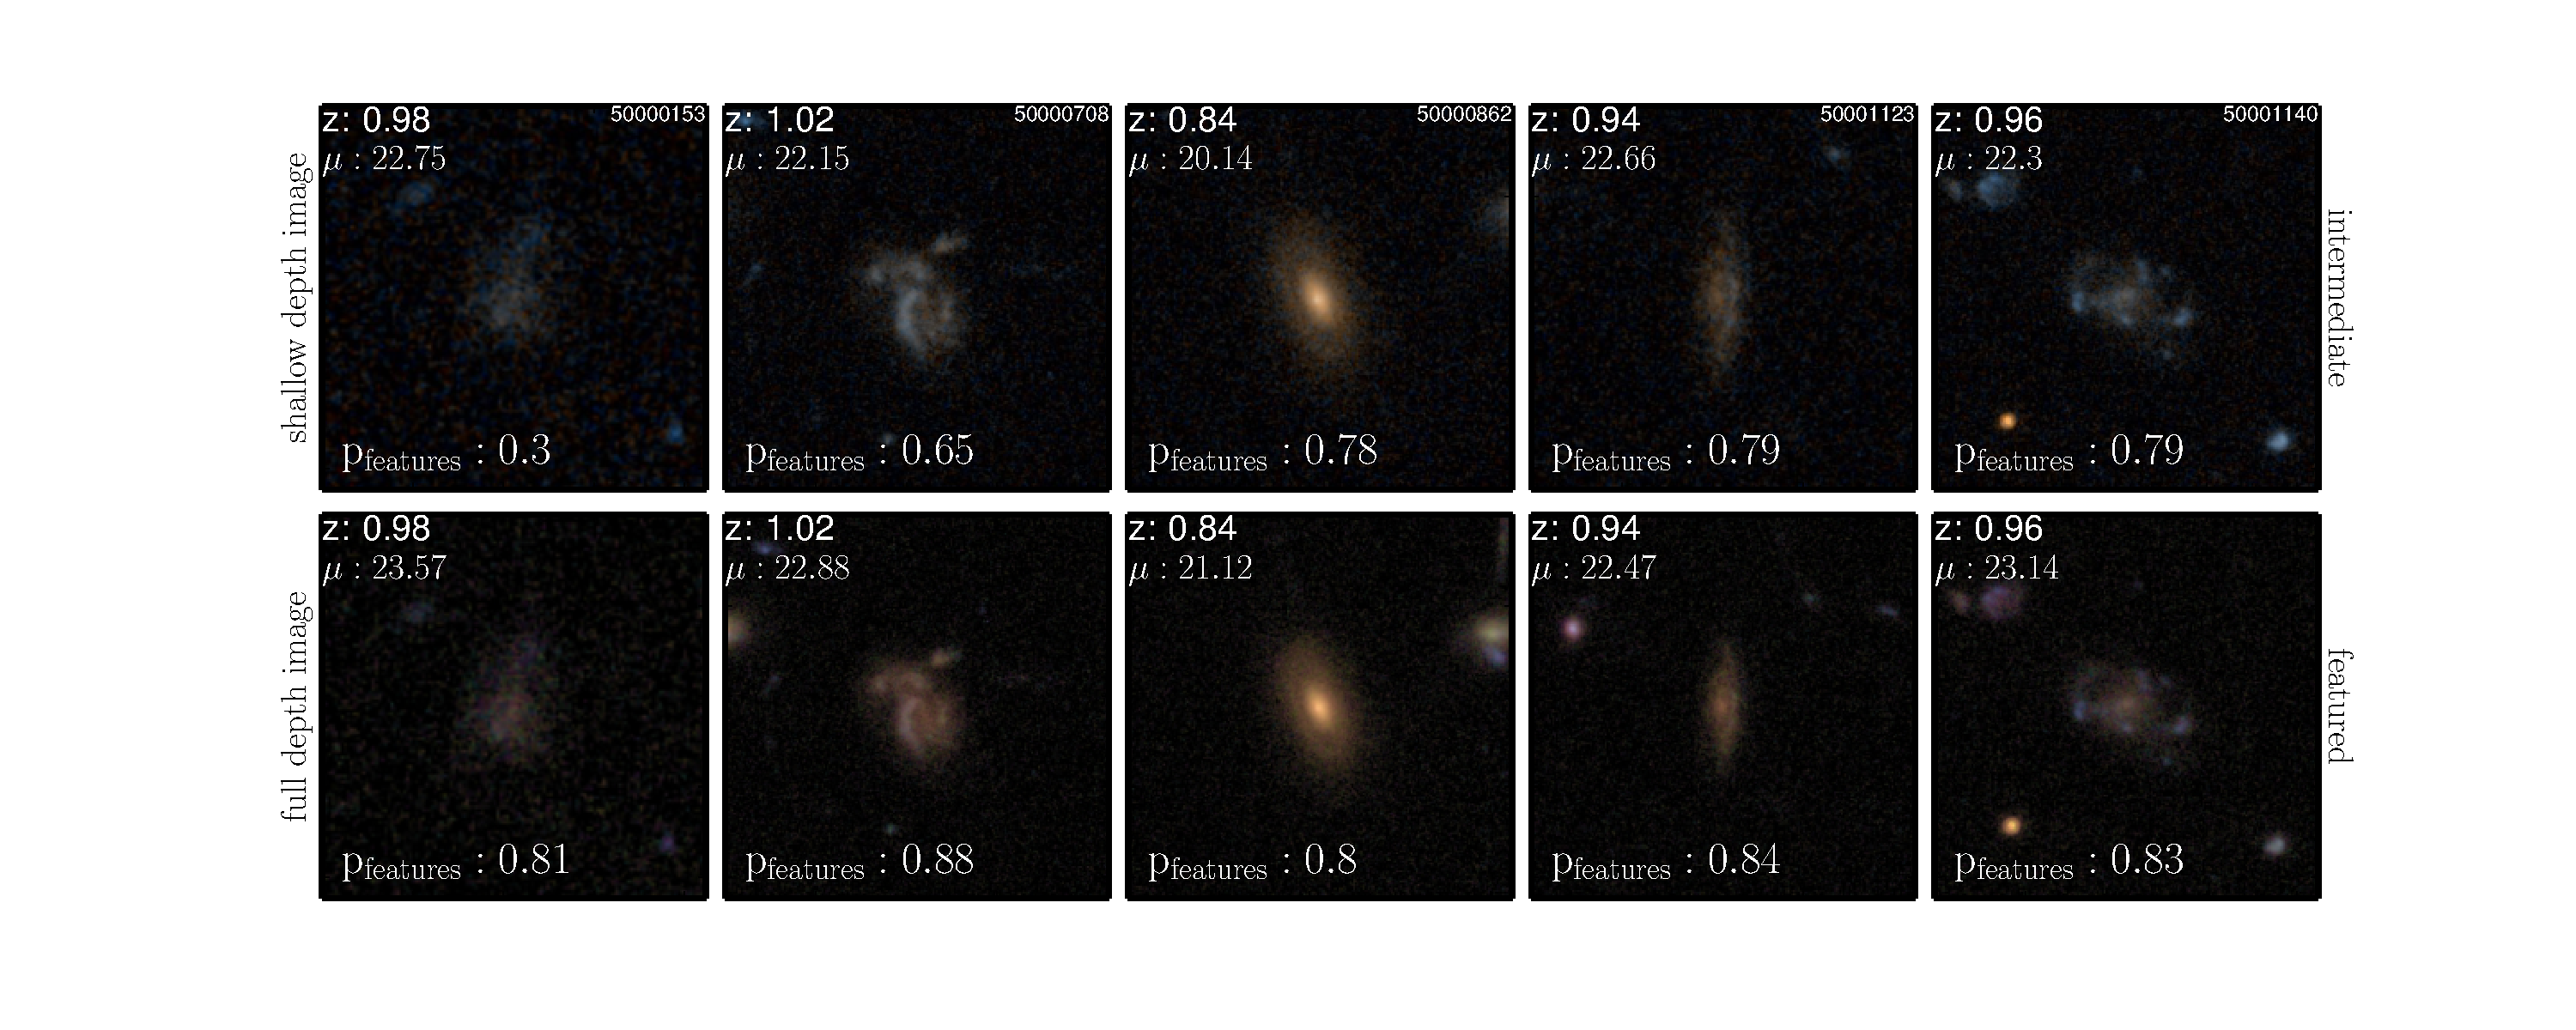
\includegraphics[width=\textwidth]{figures/intermediate_to_featured.pdf}}

\caption{Galaxies whose shallow images were classified as intermediate and full depth images were classified as smooth, intermediate, or featured.}
\label{fig:shallow_intermediate}
\end{figure*}

\begin{figure*}
\centering

\subfigure{[b]\label{fig:featured_to_smooth}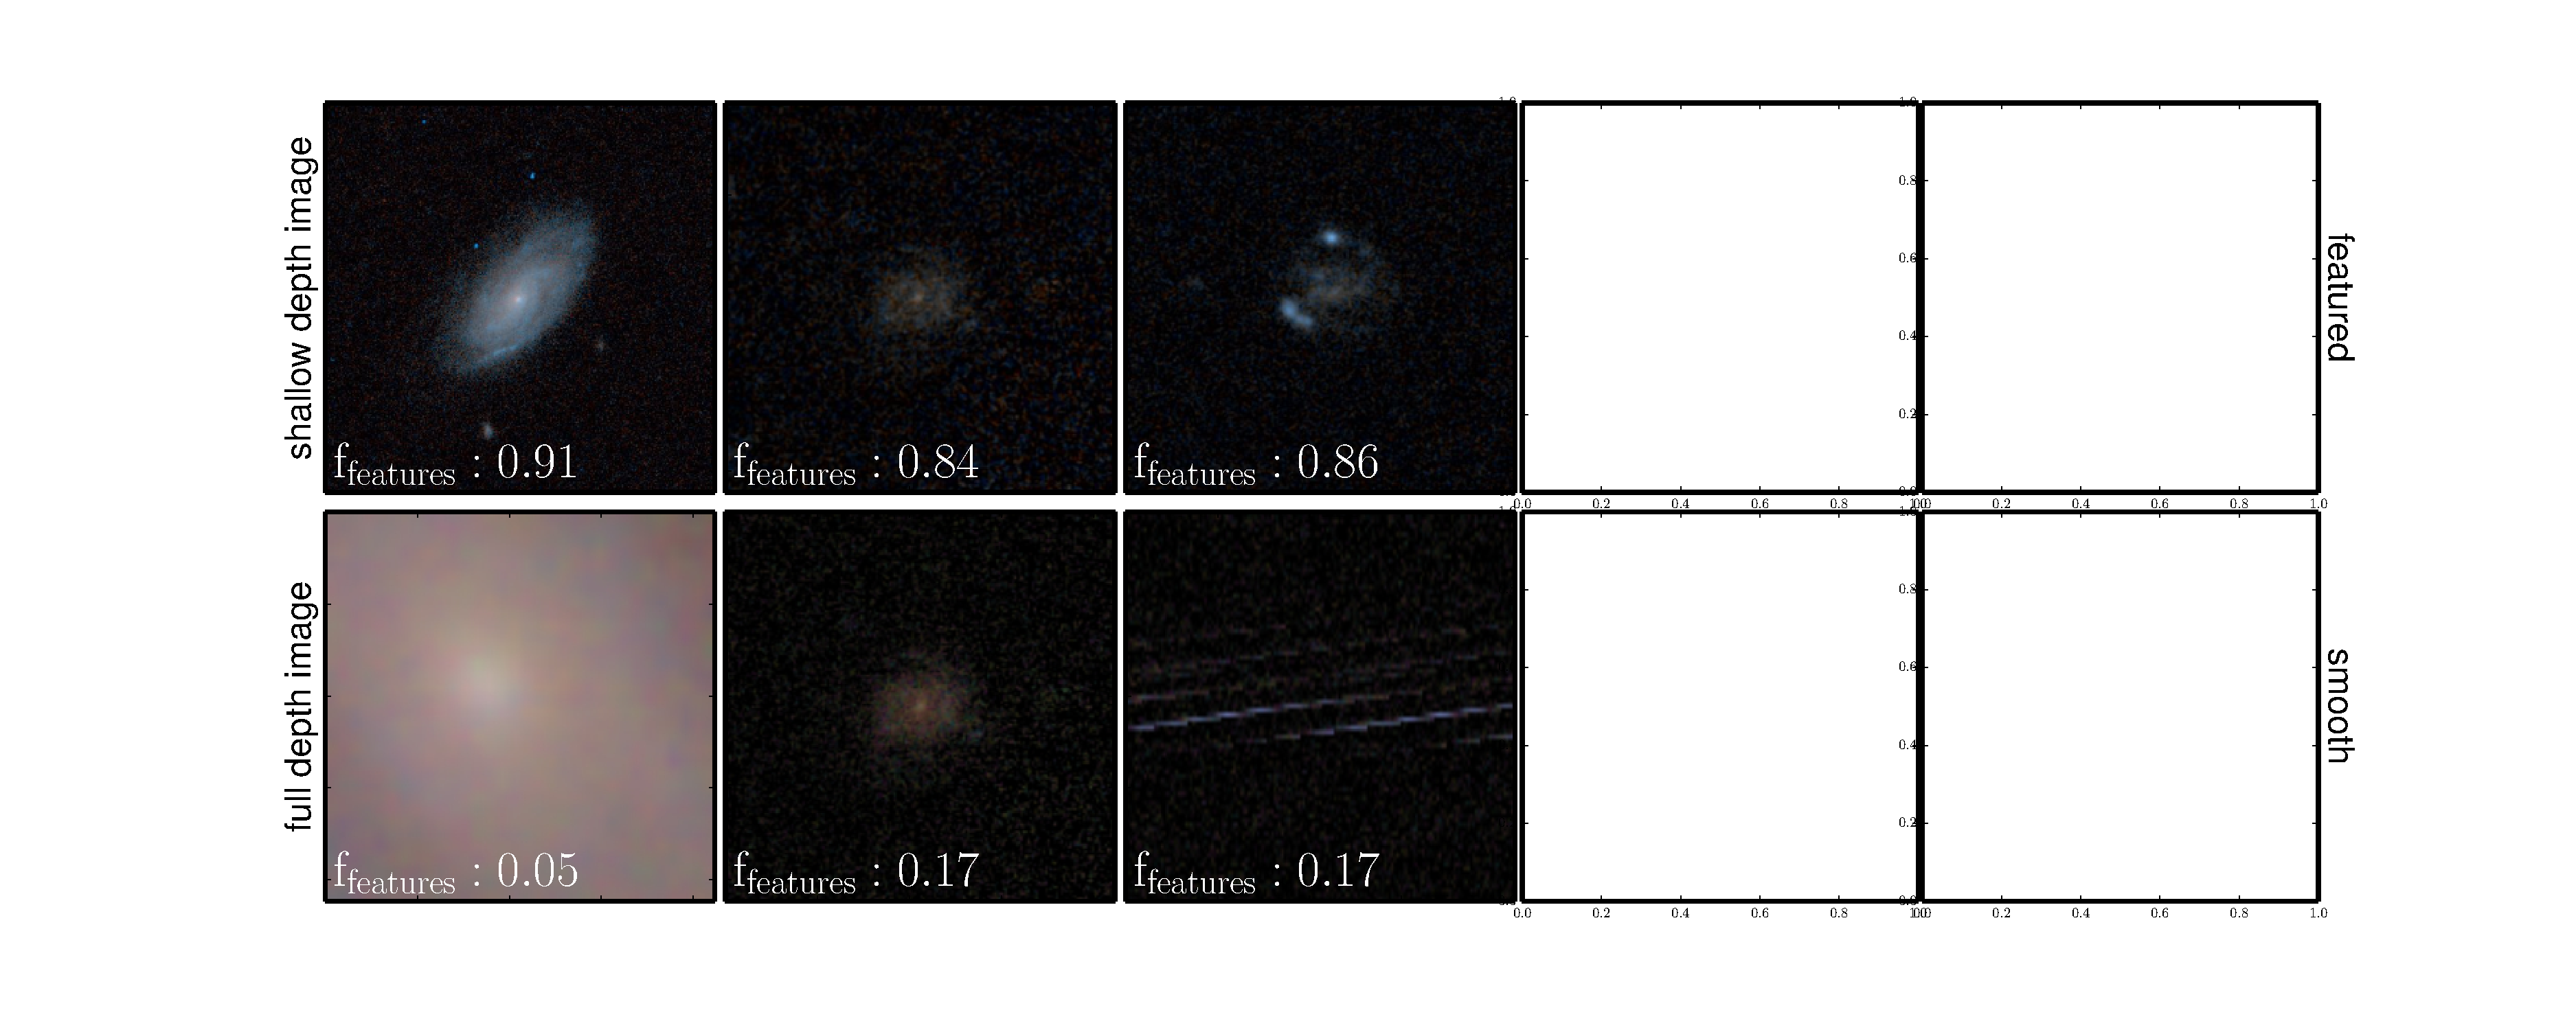
\includegraphics[width=\textwidth]{figures/featured_to_smooth.pdf}}

\subfigure{[b]\label{fig:featured_to_int}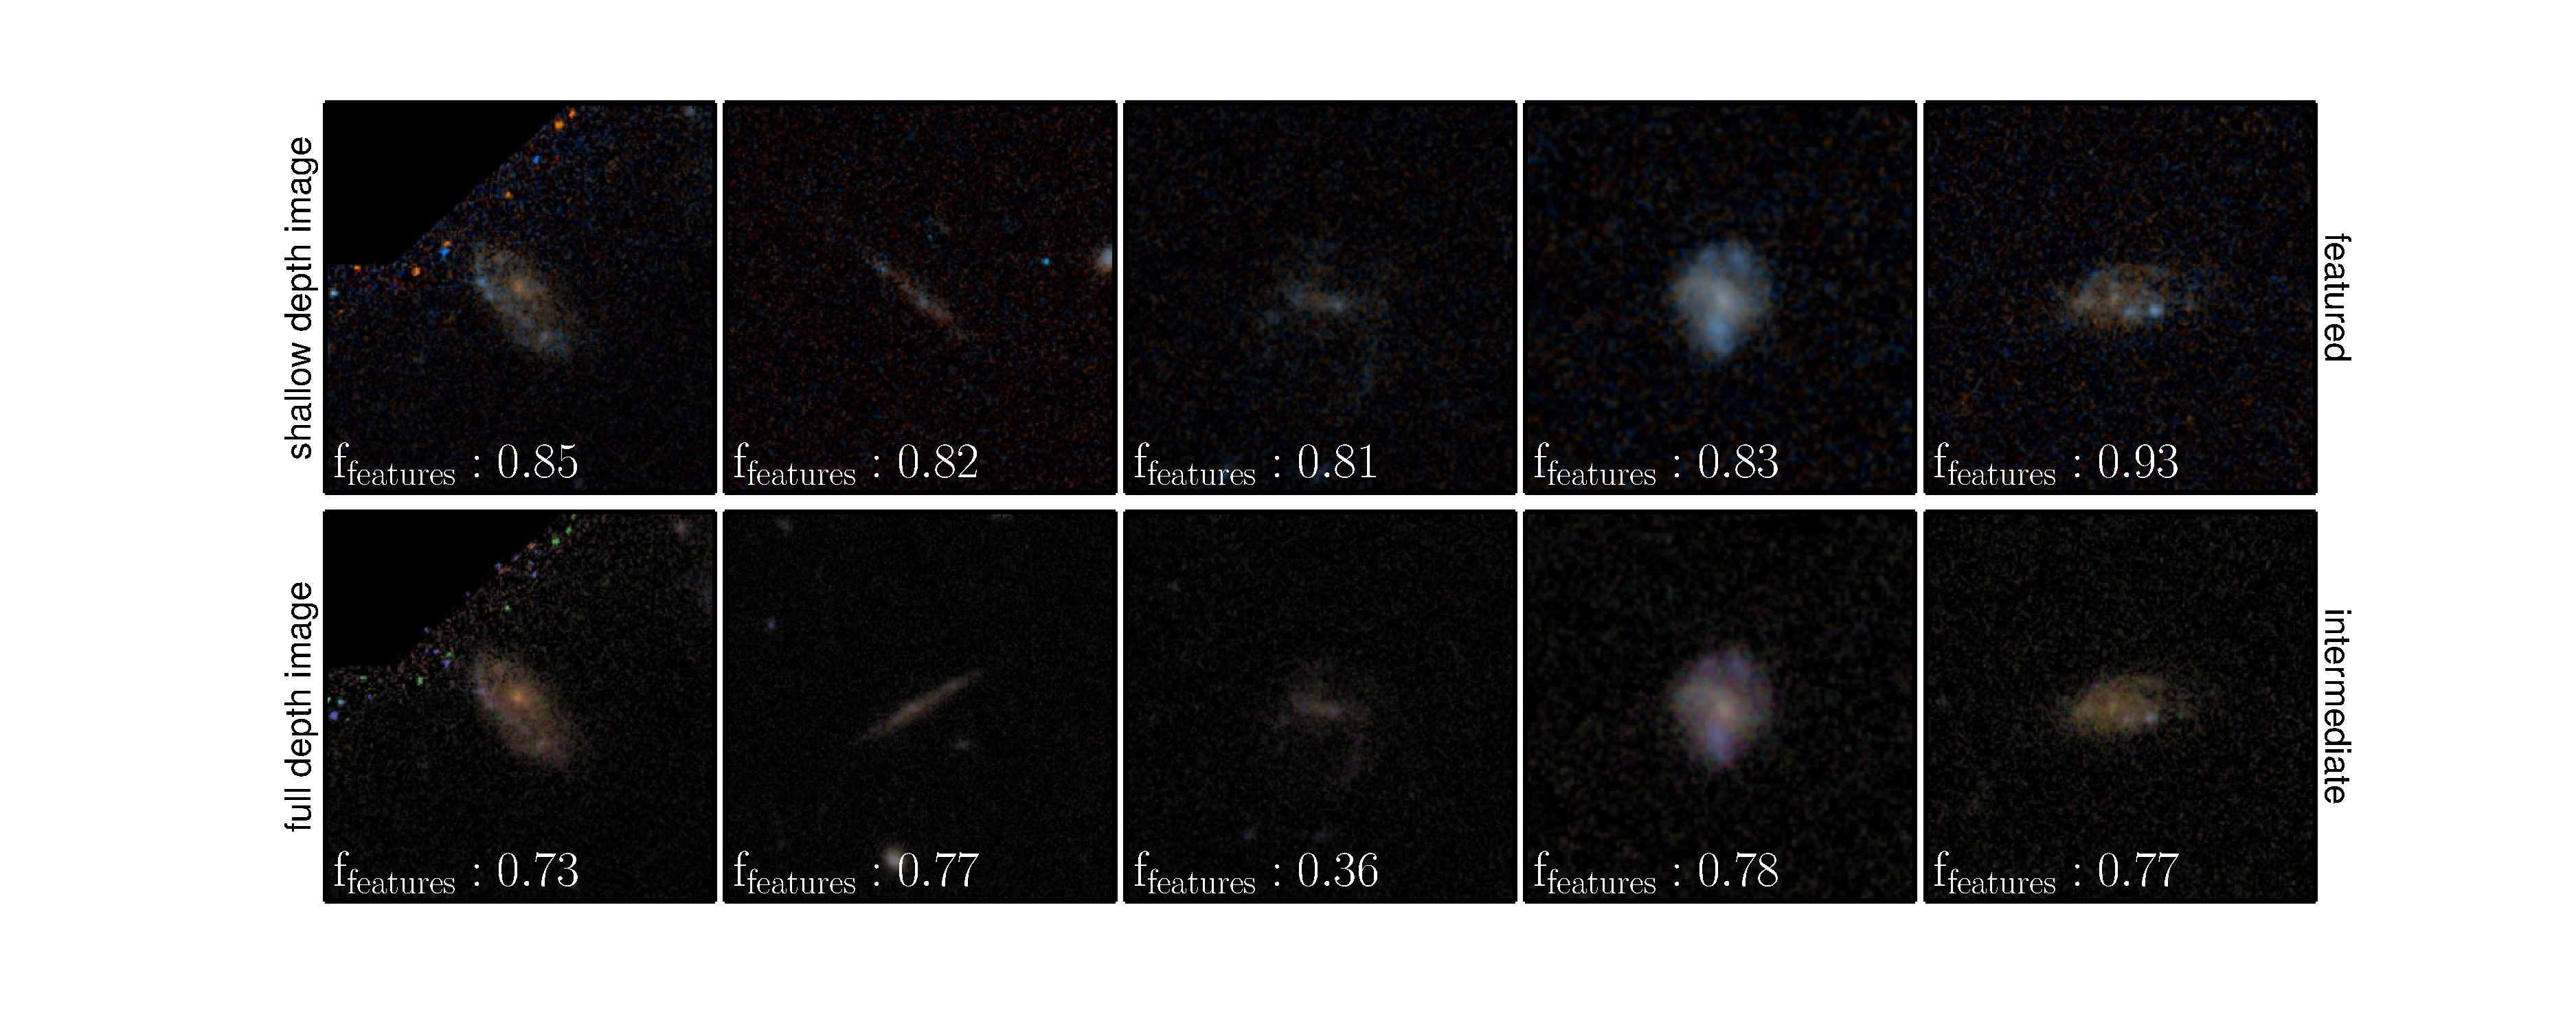
\includegraphics[width=\textwidth]{figures/featured_to_intermediate.pdf}}

\subfigure{[b]\label{fig:featured_to_featured}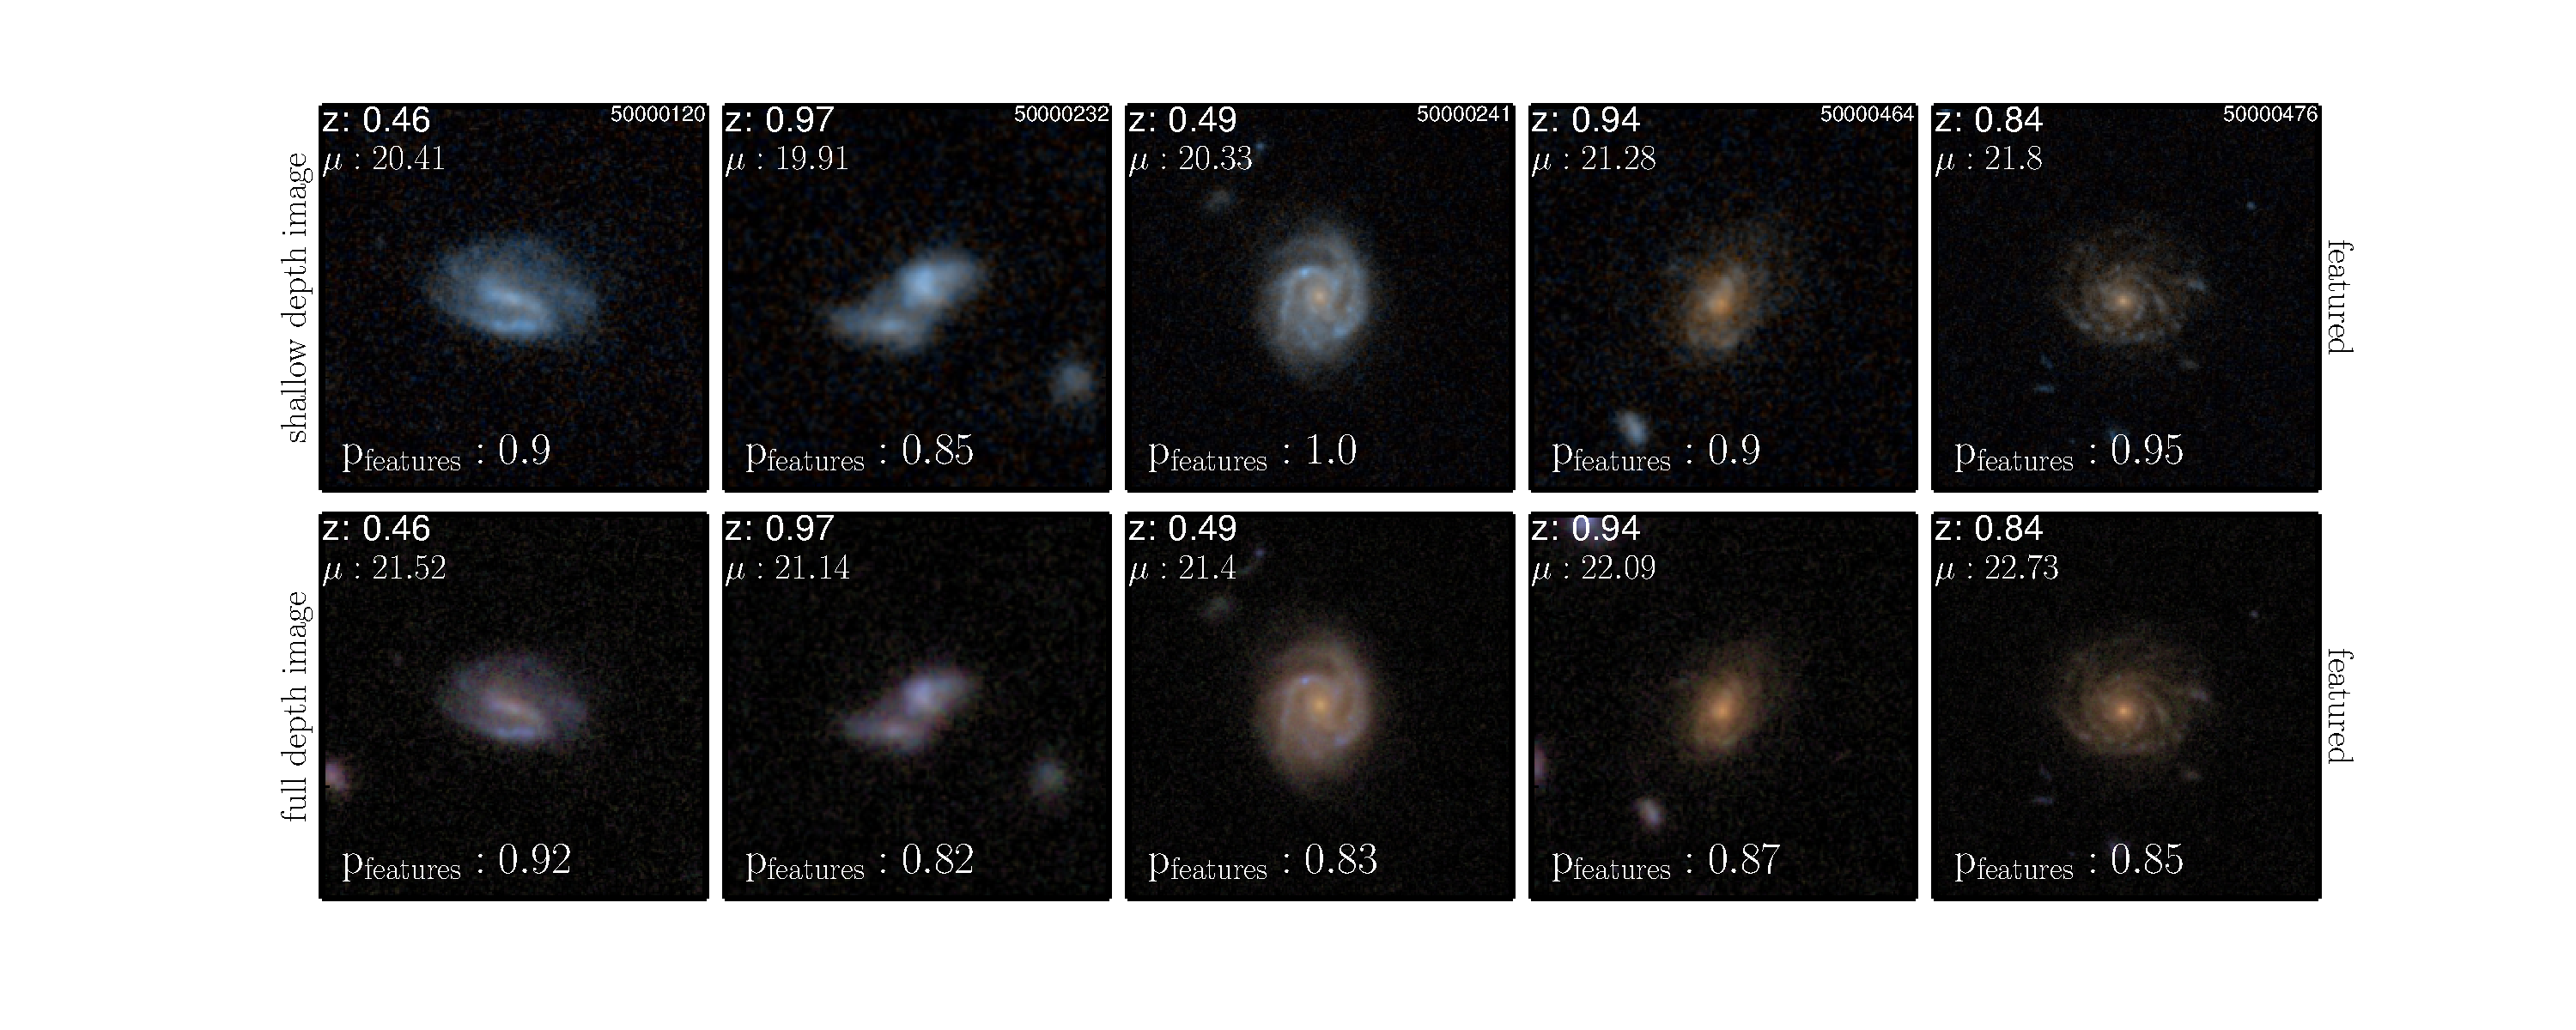
\includegraphics[width=\textwidth]{figures/featured_to_featured.pdf}}


\caption{Galaxies whose shallow images were classified as featured and full
depth images were classified as smooth, intermediate, or featured.}
\label{fig:shallow_featured}
\end{figure*}

\subsection{Debiasing higher-order tasks: \fbar}
\label{sec:ferengi_bar}

To determine the rate at which the vote fraction for any Task decreases with
redshift or surface brightness, data from simulated \ferengi{} images were
modeled with functions in discrete redshift and surface brightness bins
(Section~\ref{ssec:zeta_results}). A cut of $N>10$ was placed on the number of
votes to reduce the error in the vote fractions and ensure they were
well-sampled before applying a fit to the data. This requirement was only met
for Task~01, which significantly reduced the goodness-of-fit for the model
functions as compared with to the smooth/features task. Here we show an
example of results obtained for the bar Task. Figure~\ref{fig:f_vs_fbar}
shows that both the low sample rate and the degree of scatter in each bin
inhibit fitting a reliable function that predicts $f_{{\rm bar},z=0.3}$.
Table~\ref{tbl:ferengi_bar} summarizes the correction types for the
\ferengi{} data; 71\% of the galaxies simulated did not meet the GZH
requirements for well-sampled vote fractions for $f_\mathrm{bar}$, as
compared to 2\% for $f_\mathrm{features}$. Similar results were obtained
for all higher-order Tasks in GZH (Section~\ref{ssec:higher_order_tasks}).  

\begin{figure*}
\centering
\subfigure{[a]\label{a}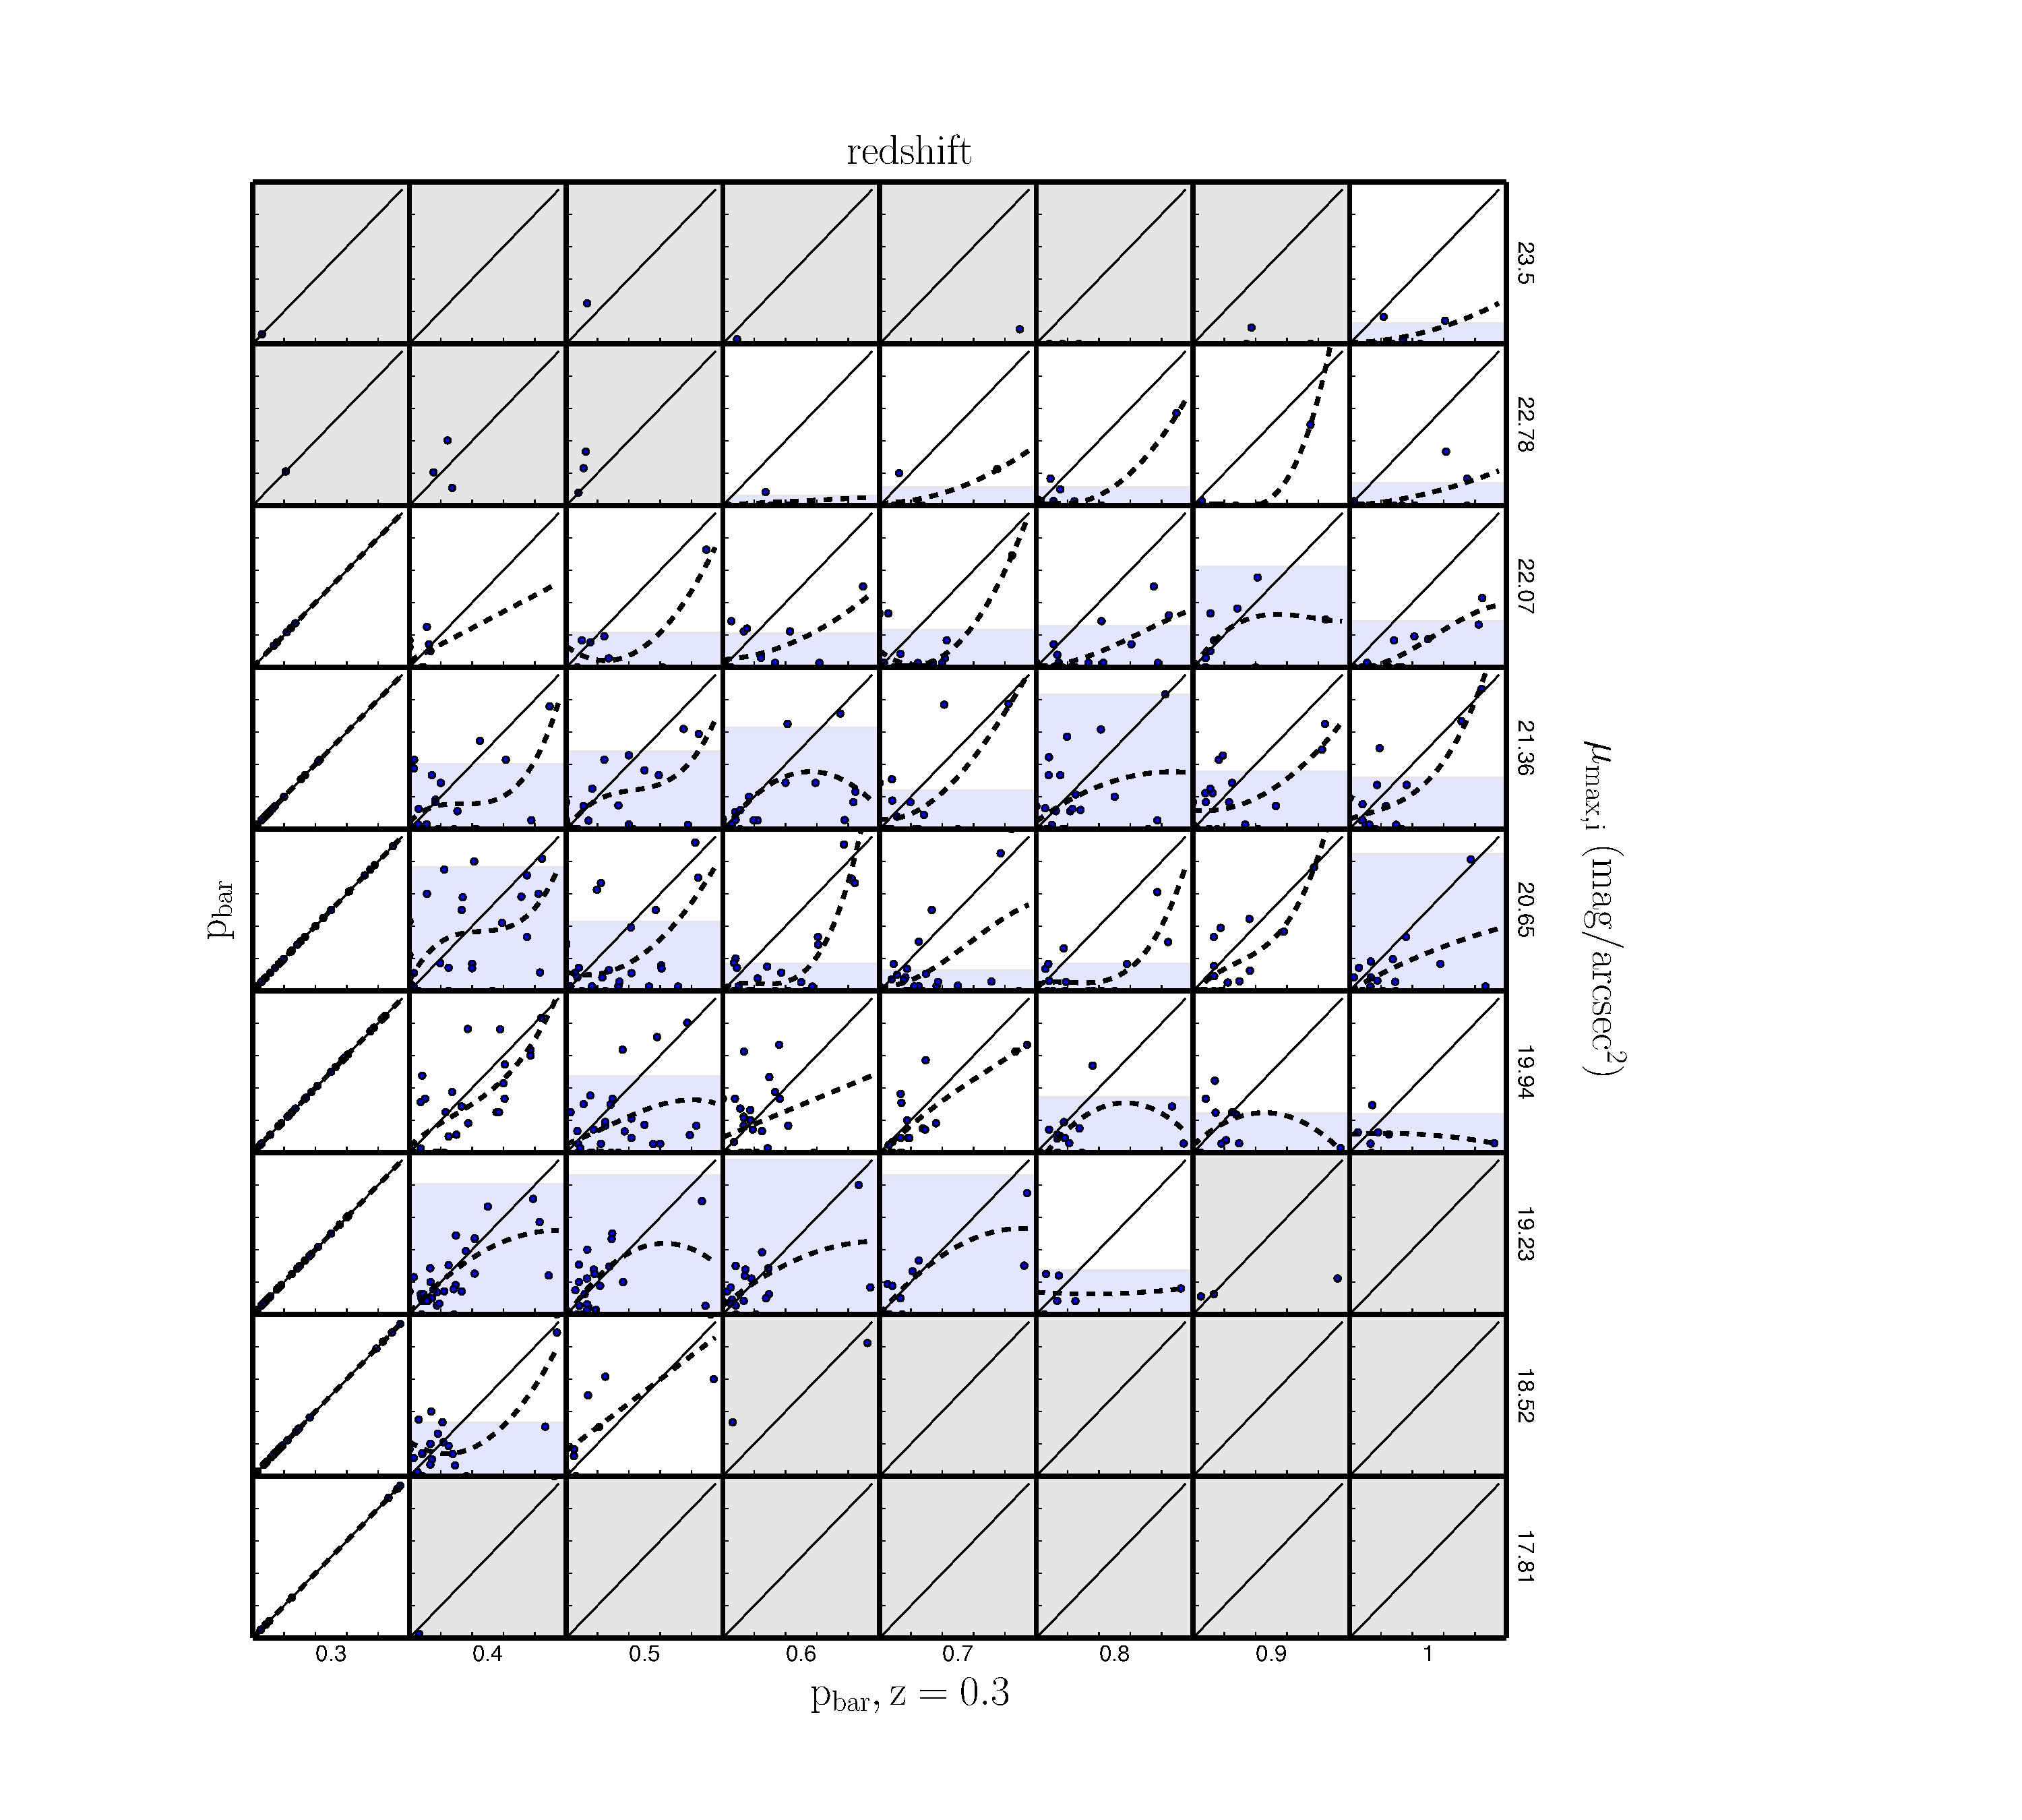
\includegraphics[width=0.5\textwidth]{figures/p_vs_p_SB_redshift_bar.pdf}}
\subfigure{[b]\label{b}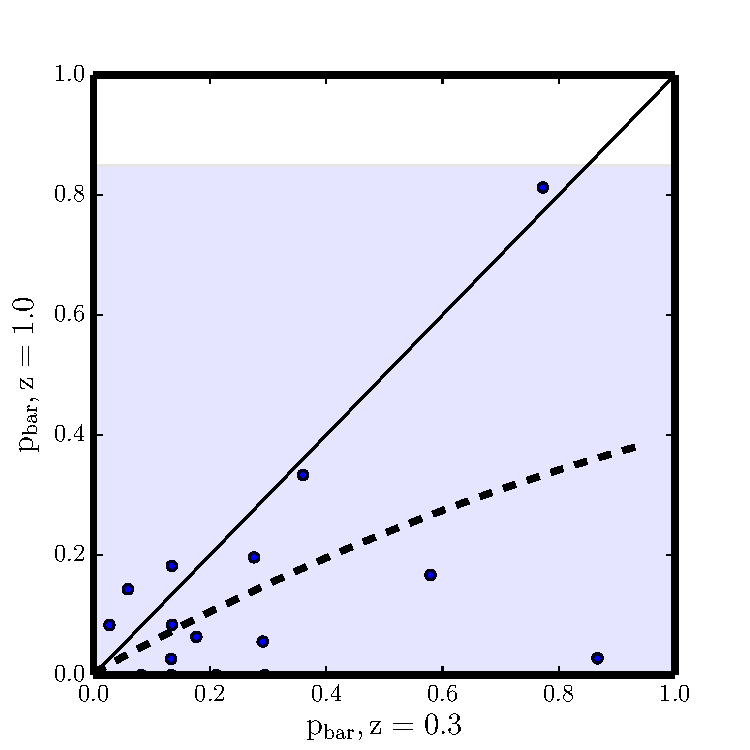
\includegraphics[width=0.4\textwidth]{figures/z1_mu20_subplot1_bar.pdf}}
\\
\subfigure{[c]\label{c}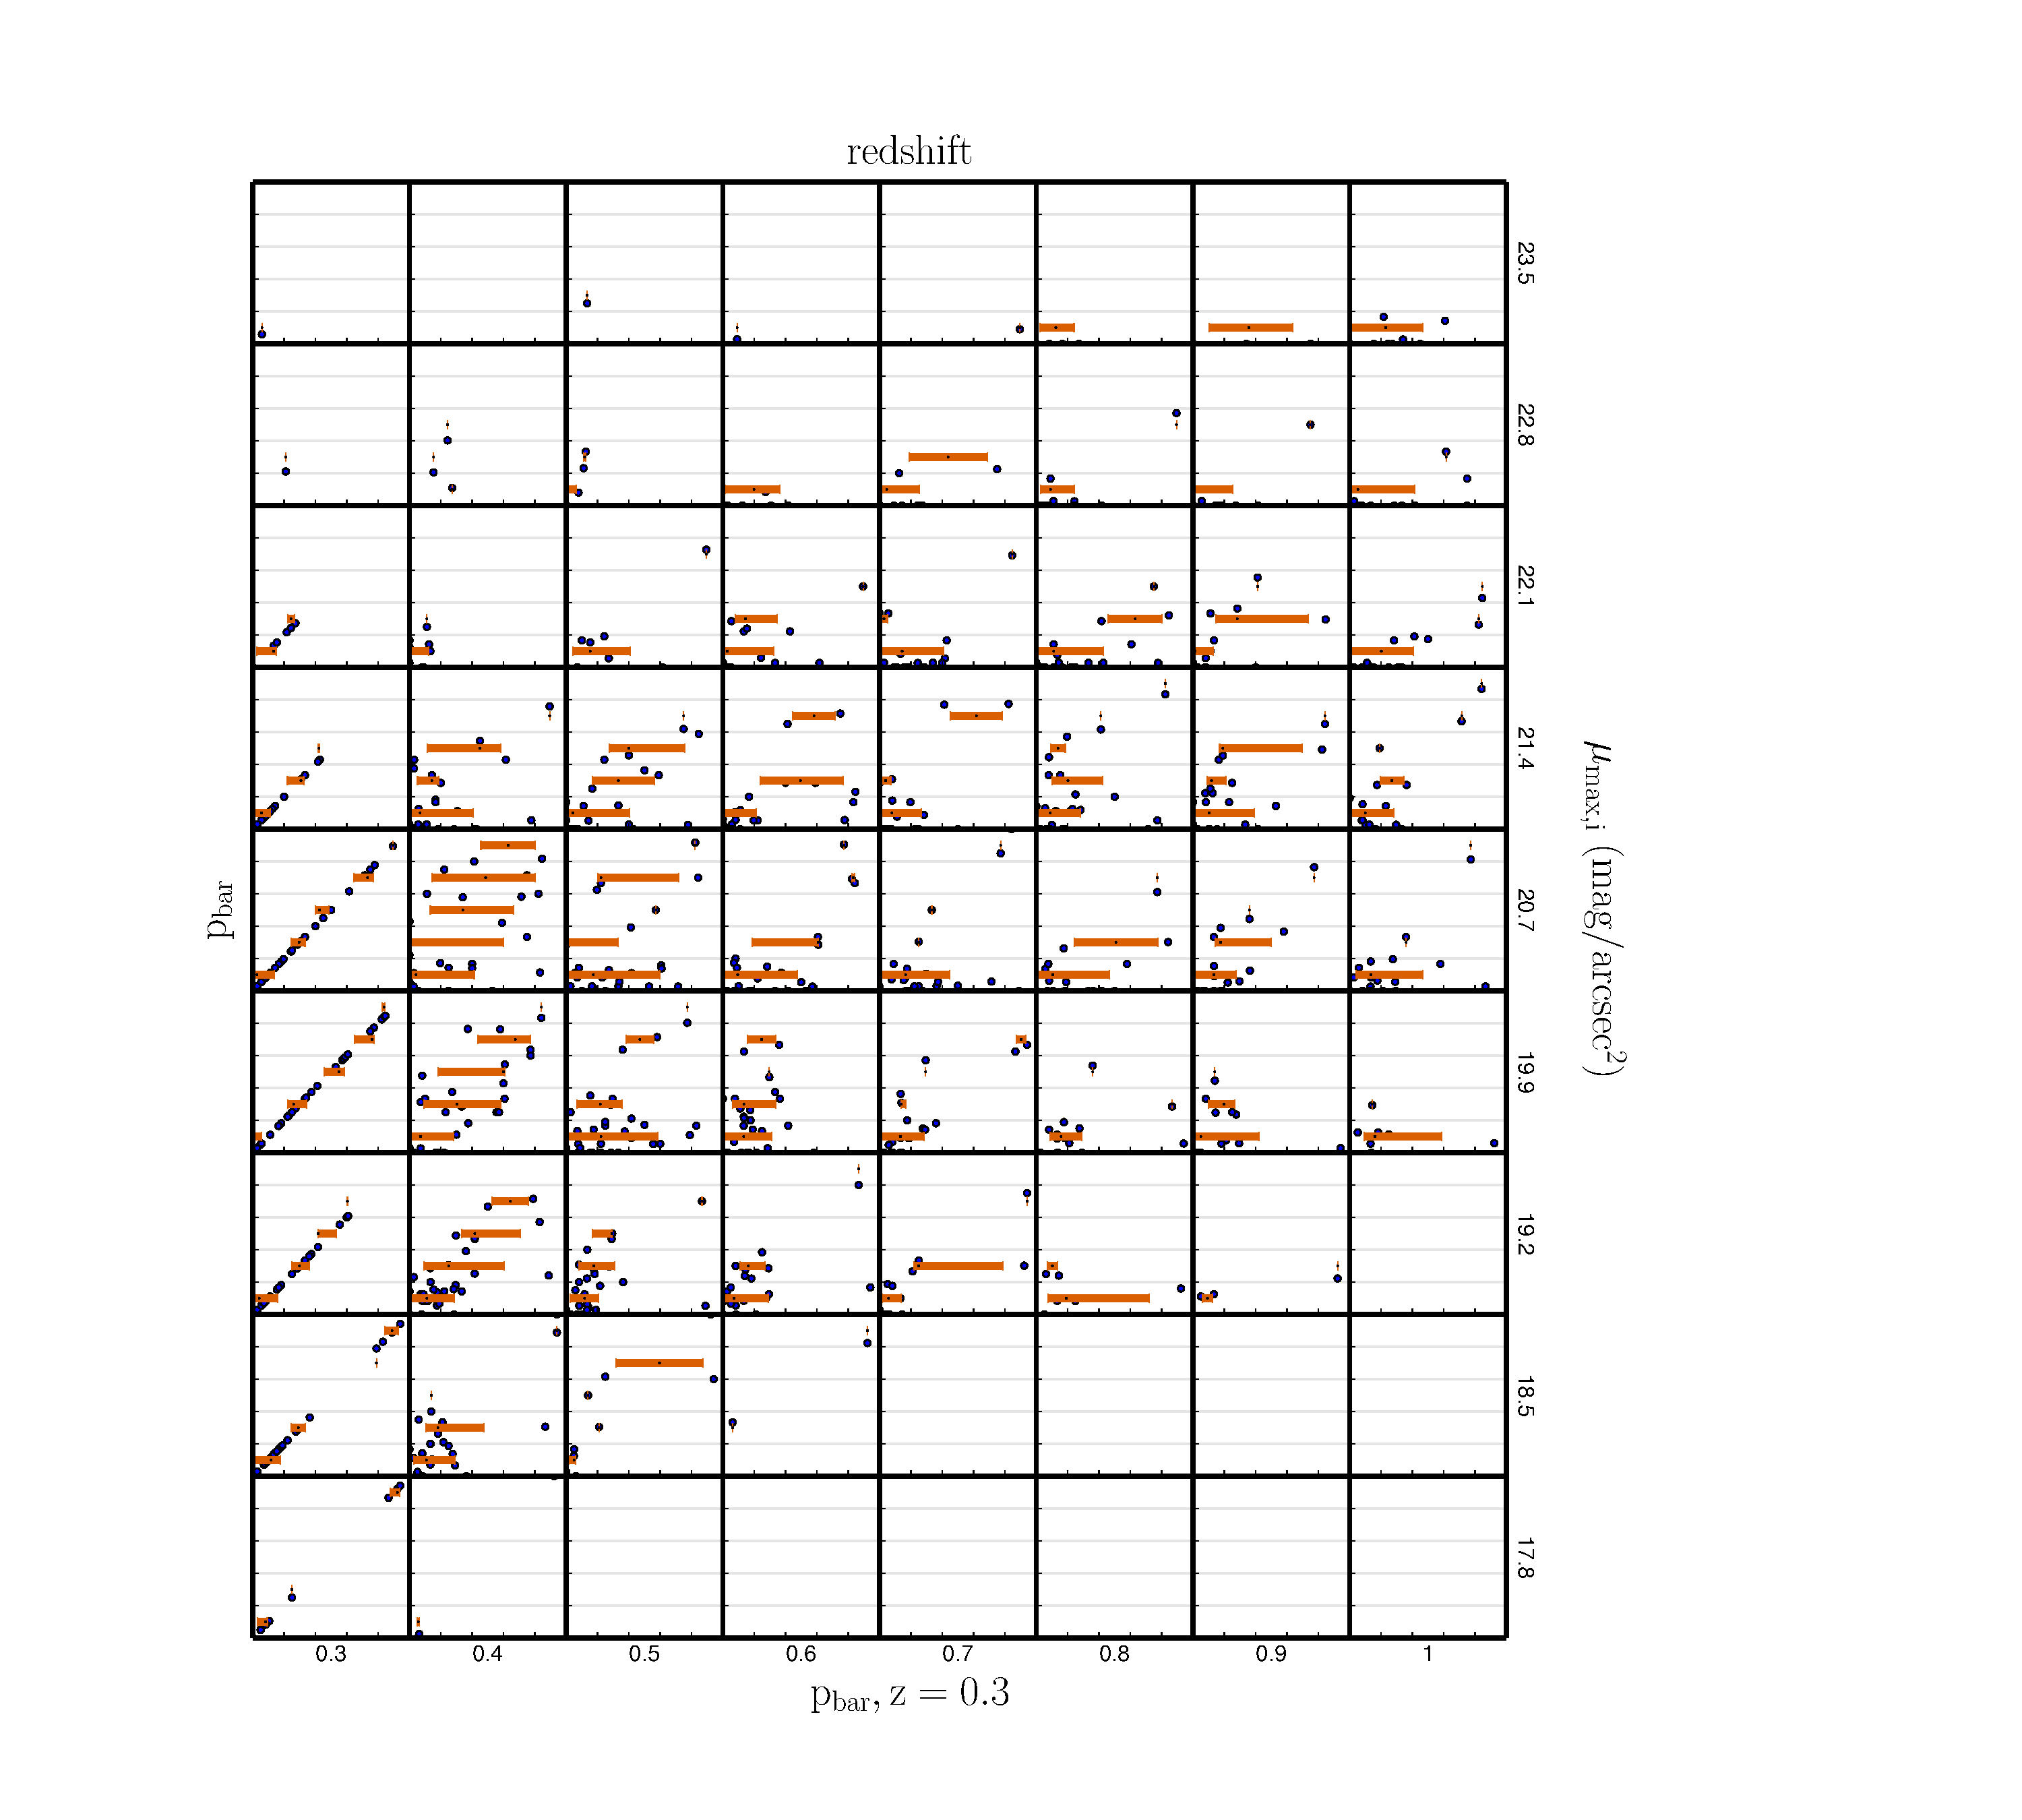
\includegraphics[width=0.5\textwidth]{figures/orangebars_bar.pdf}}
\subfigure{[d]\label{d}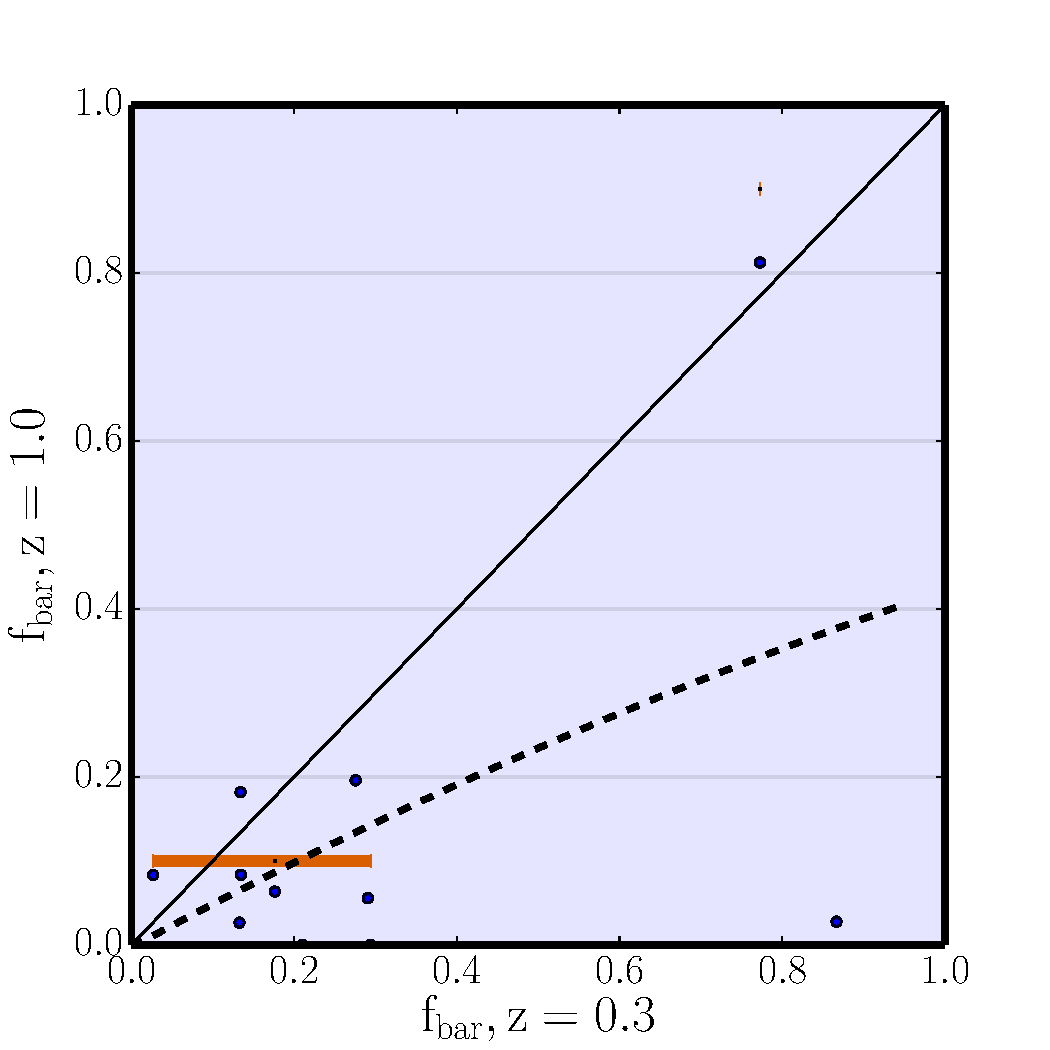
\includegraphics[width=0.4\textwidth]{figures/z1_mu20_subplot2_bar.pdf}}
\caption{Similar to Figure~\ref{fig:f_vs_f}, showing effects of redshift bias
for 3,950~images in the \ferengi{} sample. [a]: Each point in a given redshift
and surface brightness bin represents a unique galaxy. The $y$-axis in each
bin is the \ffeatures{} value of the image of that galaxy redshifted to the
value corresponding to that redshift bin. The $x$-axis is the \ffeatures{}
value of the image of the same galaxy redshifted to $z=0.3$. The dashed
black lines represent the best-fit polynomials to the data in each square.
The solid black line represents \ffeaturesz=\ffeaturesrest. Regions in
which there is a single-valued relationship between \ffeatures{} at high
redshift and at $z=0.3$ are marked in white; those in which there is not
are blue, and those with not enough data ($N<5$) are gray. The mean
normalized $\chi^2$ of the change in vote fraction is 0.08. None of the
correlations for higher-order tasks (including bars) were applied to
galaxies in the GZH catalog. [b]: A larger version of the dark-outlined
square in [a], containing \ferengi{} galaxies artificially redshifted to
$z=1.0$ and have surface brightnesses between $20.3 < \mu < 21.0$ $\rm
(mag/arcsec^2)$. [c]: The same data as [a]. Each $z,\mu$ bin is divided
into 4~sub-bins to determine the range of intrinsic \ffeaturesrest{} for a
given range of observed \ffeaturesz{} values. In each sub-bin, the orange
bars represent the inner 80$^\mathrm{th}$ percentiles of the data, the
boundaries of which are the lower and upper limits of the debiased values.
[d]: The same data as [b], but highlighting the upper and lower limit
regions.}
\label{fig:f_vs_fbar}
\end{figure*}

\begin{table}ー
\label{tbl:ferengi_bar}
\caption{Distribution of \ferengi{} images analyzed in
Figure~\ref{fig:f_vs_fbar}. Correctable images had a single-valued relationship
between their measured \fbar{} values at high and low redshifts (white regions
in Figure~\ref{fig:f_vs_fbar}). Galaxies with a lower-limit on \fbar{} had a
non single-valued relationship (blue regions). NEI images had undetermined
relationships due to a lack of data ($N<5$) in their corresponding $z$-$\mu$
bins (gray regions). Only 17\% (maximum) of \ferengi{} galaxies in the sample
were considered ``correctable'', which is not sufficient to compute a $\zeta$
function applicable to the Hubble data.   \label{tbl:ferengi_bar_corrections}}
\begin{tabular}{lrr}
\hline \hline
				                   & N       & \% \\
\hline 
Correctable                        & 664   & 17\% \\
Lower-limit                        & 483   & 12\% \\
NEI                                & 2,803     & 71\%\\
Total                              & 3,950   & 100\% \\
\hline \hline
\end{tabular}
\end{table}


\end{document}

